\pdfoutput=1

\documentclass{l4proj}

% put any packages here
\usepackage{graphicx} 
\usepackage{subcaption} %  for subfigures environments 
\usepackage{pdfpages}
\usepackage[hyphens]{url}
%

\begin{document}
\title{SteamVR Assistant - Virtual Reality Development Toolkit}
\author{Joseph O'Hagan}
\date{March 28, 2018}
\maketitle

\begin{abstract}
This project focuses on the creation of a virtual reality development toolkit aimed at non-technical developers. The SteamVR Assistant (SVRA) provides a simple to use, development toolkit for non-technical developers working with the HTC Vive headset and the Unity game engine. It provides a code free development experience by providing the development of virtual reality applications through the Unity engine's graphical editing tools. 

In this report we first begin by contextualising the current state of the virtual reality industry and providing the motivation for the project. Afterwards the aims of the product, which were based on an interview held with non-technical virtual reality developers, are specified. The design of the product in terms of the preliminary, usability and technical decisions made is then discussed. An explanation is given of the product's implementation, followed by a discussion of the evaluation methods which the product underwent during development, specifically two rounds of participant evaluation and an expert interview. Finally the report concludes by discussing the future work and direction of the product and by summarising the goals and accomplishments of the project. 

\end{abstract}

\educationalconsent
%
%NOTE: if you include the educational consent (above) and your project is graded an A then
%      it may be entered in the CS Hall of Fame
%
\tableofcontents
%==============================================================================

\chapter{Introduction}
\pagenumbering{arabic}
This chapter provides a background of virtual reality to contextualise the current state of the industry. It then outlines the motivation of this project from both a consumer and academic perspective. From this the aims of the project are drawn and an outline of the remaining contents of the report provided.  

\section{The Current State of the Virtual Reality}
\label{sec:introductionbackground}
Virtual Reality (VR) is not a new concept. A significant amount of research during the late 1960’s and 1970’s formed the basis by which VR appears today \cite{Sutherland65theultimate}, \cite{Sutherland_ahead-mounted}, \cite{ResponseEnviron}. The most seminal of these works being Ivan Sutherland's ``The Ultimate Display'' in which the key concepts of immersion within a simulated world and complete sensory input and output were introduced. It was not until the 1980s however that the different technologies required for the development of VR converged to allow for the creation of the first true VR systems. It was at this time that a team of researchers at the Massachusetts Institute of Technology developed a limited three-dimensional virtual workspace in which the user interactively could manipulate 3D graphical objects spatially corresponding to their hand position \cite{MIT}. It was also at this time that development of VR projects began outside of academic institutions with NASA, for example, starting the VIVED project (Virtual Visual Environment Display) and later the VIEW project (Virtual Interactive Environment Workstation).

Although significant research, development and public interest \cite{RandyDisney} surrounded VR during the 1990s the immersive VR experiences envisioned failed to breakthrough into the consumer market with \cite{mark} positing a number of reasons for this failure. Firstly the technical quality of the Head-Mounted Displays (HMDs) at the time was considered poor (in terms of resolution, field of view, weight and motion sickness), socialization was also not facilitated (as users felt uncomfortable being unable to interact with others), the graphical quality of the rendered scenes was inadequate, and the cost of the devices prohibitive. Due to these factors and the technology's inability to maintain pace with the unrealistic expectations and portrayals of it in media, the consumer VR devices (such as Nintendo's Virtual Boy\footnote{A consumer 32-bit video game console released by Nintendo in 1995}) failed on the consumer market. 

Despite this failed consumer launch of VR, research and development continued in the medium at a steady pace as technical and software advancements saw many of the longstanding issues of VR (such as hardware complaints, comfort, motion sickness, etc.) being addressed. Such developments were the driving force behind a resurgence of the medium for both work and entertainment \cite{mark} as increased levels of investor and consumer interest continued to grow, with the acquisition of Oculus\footnote{An American technology company founded in 2012} by Facebook for \$2bn in 2014 being herald as the evidence that VR had returned indefinitely as a consumer product. This acquisition brought about a significant increase in venture capital investments being made in VR and Augmented Reality (AR) products, with 2016 seeing the first major consumer launch of VR devices onto the marketplace. 

Investigating the current state of VR devices, both a Goldman Sachs study \cite{Goldman} and BOM report \cite{BOM} agree that the technology required for VR devices is ready for consumer VR devices to exist on the market. Instead they suggest that consumer content is what's needed most for the devices and medium to thrive. This sentiment is reinforced by additional studies such as the CAICT's 2017 Virtual Reality / Augmented Reality White Paper \cite{WhitePaper}  which agree that the VR industry currently compiles with the ``hardware-content'' development pace, where hardware forms the foundation and the content is used to improve the user experience. This stance is also taken by Gartner's ``Emerging Technology Hype Cycle'' which models the hype cycle for a new technology. An example of such a hype cycle is found in Amara's law which states that \textit{``We tend to overestimate the effect of a technology in the short run and underestimate the effect in the long run.''}.

\begin{figure}[h]
\centering
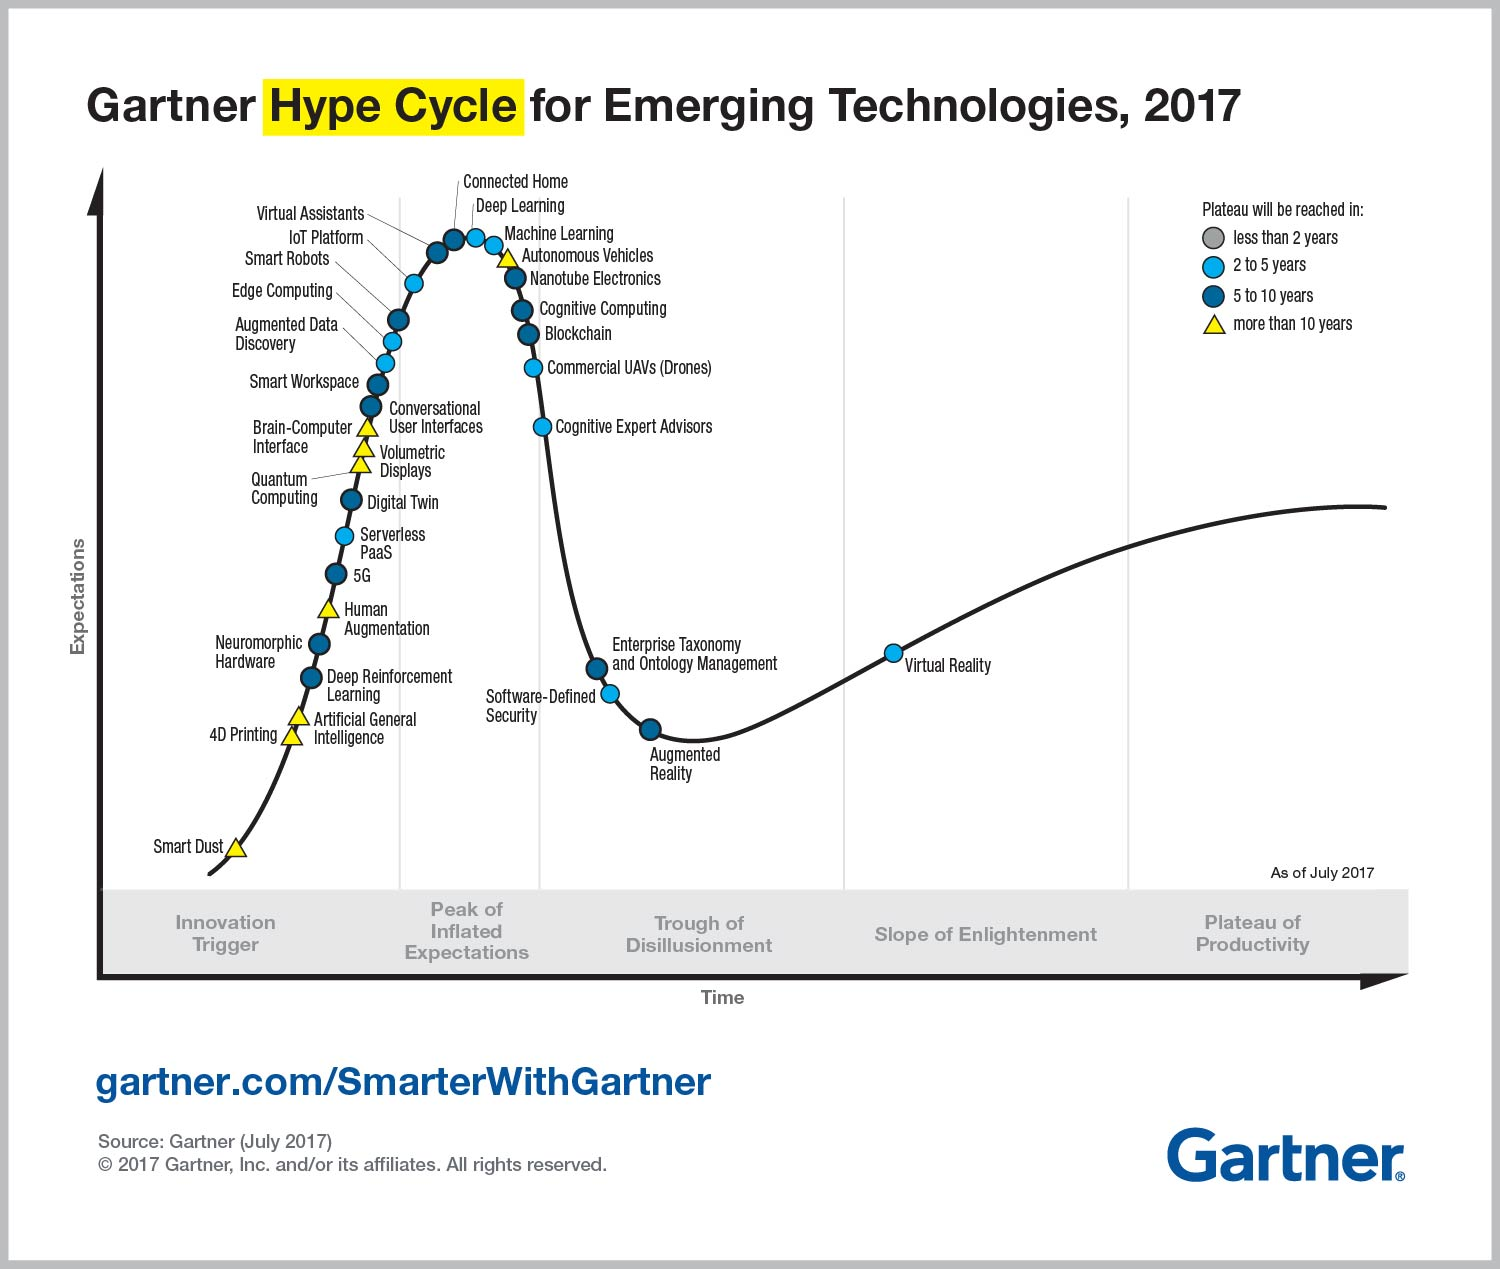
\includegraphics[height=10.2cm,width=14.2cm]{dissertation/gartner_hype_cycle.jpg}
\caption{To Do}
\label{gartner_hype_cycle}
\end{figure}

This is trend was most recently seen with virtual reality where the failed initial launch of the technology and its recent relaunch onto market with the release of the HTC Vive\footnote{Developed by HTC and Valve Corporation and released in 2016}, Oculus Rift\footnote{Developed by OculusVR and released in 2016} and Sony's PlayStation VR\footnote{Developed by Sony Interactive Entertainment and released in 2016} being met with exaggerated claims of the impact of the technology in the near future. In reality what occurred was the exaggerated expectations were swiftly followed by claims that the medium had once again failed to establish itself on the consumer market. However with the continued rise of users, content development and release of new VR devices the industry is working towards its ``Plateau of Productivity''. As outlined by the above graph the technology is steadily working towards its point of widespread usage and impact. Where before hardware development was the focus, what matters now is the development of new content and ideas as the shift in importance transitions from hardware improvements to the improvement of perception, interaction and content creation going forward. 

\section{Consumer Motivation}
\label{sec:introductionmotivation}
Following the ``hardware-content'' development model proposed in the \cite{WhitePaper} it is the content creators who play the most significant role if the VR medium is to prosper. Currently the lead content creators for VR are found within the entertainment industries, with the video game industry being identified as the most impactful within the next three years by a 2017 VR Intelligence industry survey \cite{VRX}. The proposed ``hardware-content'' pace seen of VR devices closely mimics that seen within the video game industry when a new video game console, a hardware platform for playing video games, launches onto the market. When a new hardware platform launches the developers creating the content initially are limited due to the lack of tools available for development while the developers are still gaining a better understanding of developing for the new hardware. Despite existing, cross-platform, tools such as the Unity\footnote{A cross-platform, publicly available game engine developed by Unity Technologies} and Unreal\footnote{A cross-platform, publicly available game engine developed by Epic Games} game engines being available to streamline development for the new platforms, development remains challenging. The same is found of VR development as developers can make use of existing tools such as the Unity or Unreal game engines in addition to VR development libraries built into the existing toolchains and custom extensions made by developers. The development process, however, remains labour intensive, expensive and often requires extensive technical knowledge. This immediately creates a barrier to  entry for many interested developers who lack the necessary background knowledge or resources for development. 

VR development also brings new unforeseen challenges to developers. Figuratively a ``return to Pong'' developers creating VR applications must discover new best practices due to the paradigm shift away from traditional applications to the immersive experiences provided by VR. Furthermore VR currently suffers from what can be viewed as the ``chicken-and-egg'' dilemma between developers and consumers. The aforementioned VR Intelligence industry survey suggests that the biggest barrier for mass consumer adoption of VR is the price of the devices and the lack of available content. Meanwhile the developers are hesitant to develop VR content due to the high development costs and small consumer install base. Hardware costs aside, the consumers are reluctant to buy into the technology due to the lack of content while the developers are hesitant to develop content due to the lack of consumers.

One solution to this problem is to reduce the barriers for entry required for development, whereby encouraging more developers to try and make VR applications. There are various possible approaches to this but the one focused on in this project is to reduce the required technical knowledge of developers thus encouraging more non-technical developers to create content. In doing so a cheaper and faster development cycle is also created which too encourages developers. Encouraging developers to create new content leads to new best practices for design and improved experiences, which in turn increases the consumer install base, which encourages the number of developers, et al. 

\section{Academic Motivation}
\label{sec:introductionacademicmotivation}
Aside from as an entertainment device, a significant interest in VR exists from an academic perspective. Human Computer Interaction (HCI) currently has an increasing interest in the artistic and cultural applications of computing, but this requires working alongside artists to create and study public experiences in settings such as theme parks and the city streets \cite{drthesis}. Much work has been done in the past two decades exploring and creating many collaborative, cross-sector projects between computer scientists and artists though less has sought to investigate the potential for collaborations between the arts and commercial digital industries despite being seen as a valuable opportunity \cite{drthesis}. Collaboration between the artists and HCI researchers remains difficult however \cite{drwbenford} \cite{drweng2}, as both parties draw on methodological legacies in their approaches. Where the artistic creative practice involves the creation of something new and perhaps unexpected, the scientific perspective relies on the need to collect and analyse information in a more systematic and generalisable way. Bringing both perspectives together to generate both new knowledge and artistic artifacts requires devising new methods of collaboration. 

One of the major problems of this working relationship is that the intent of one party is not met by the other due to the paradigm shift between the two mediums. Where an artist might describe their envisioned application to the HCI developer the created application might fail to meet the artist's original intent. This failure to capture the artist's vision may be due to technical difficulties experienced by the developer or alternatively could be due to a communication misunderstanding between the artist and the developer. For the latter problem, one solution is to involve the artists more in the creation of the application itself by allowing the artist to create a simple prototype application to better show their intended application to the developer. Currently no method exists for a non-technical developer, such as a artist, to easily create a simple, prototype VR application. Existing tools instead require extensive technical knowledge and often require a significant time investment of the user to learn and then create their application. Instead what is needed is a simple development tool aimed at non-technical developers which would allow them to quickly experiment and prototype applications which may be then used as a proof of concept, throwaway prototype or as the base for the development of a much larger, complex application by more technically capable developers.

\section{Project Aim}
\label{sec:introductionprojectaims}
The aim of this project is to develop a Unity VR development toolkit targeted at non-technical developers working with the HTC Vive. The project aims to develop a Unity library suitable for artists and users with little to no prior technical knowledge but are interested in developing VR content. It aims to achieve this by providing users with a range of tools which can be used exclusively through Unity’s graphical editing tools. The project also aims to create an easily extendable toolkit so that developers with a technical background can easily customise the toolkit to the particular needs for their envisioned application.

\section{Outline}
\label{sec:introductionoutline}
This report contains the following structure:
\begin{itemize}
    \item \textbf{Chapter 2 - Context \& Related Work:} Provides the necessary background context for the project and a survey of the similar, existing toolkits currently available.
    \item \textbf{Chapter 3 - Requirements:} Discusses the project's requirements and aims and the methods in which they were elicited.
    \item \textbf{Chapter 4 - Design:} Discusses the preliminary, usability and technical design decisions made during the development of the product.
    \item \textbf{Chapter 5 - Implementation:} Describes the implementation of the project in detail.  
    \item \textbf{Chapter 6 - Evaluation:} Discusses the three rounds of evaluation which were performed on the product and the changes made in response the feedback received.
    \item \textbf{Chapter 7 - Conclusion:} Outlines suggestions for future work and potential directions for the product and summarises the project's development and its achievements.
\end{itemize}

\chapter{Context \& Related Work}
\label{sec:contextchapter}
This chapter provides a survey of the existing tools available to developers interested in creating VR content. While not complete, it presents a comparison of two of the most popular tools available to developers. It also provides a description of the purpose of a game engine in the content creation process and discusses an alternative game engine which could have been used during the development of this project. 

\section{Game Engines}
\label{sec:contextgameengines}
Prior to the advent of game engines, video games were typically created as singular entities. Often a game for a specific platform was required to be designed from the bottom up to make optimal use of the hardware with very little resources being reused between games. Development also required the developer have extensive technical knowledge of low level programming languages or the hardware’s assembly language in order to create their game. To streamline development and reduce development costs, developers created game engines as a software framework to assist with the creation and development of video games. 

A game engine exists to abstract the details of doing common game-related tasks to allow developers to focus less on the technical concerns of development but rather on the design decisions which make their games unique. They provide reusable components which can be used or adapted to create different games. Typically the functionality provided includes a rendering engine, a physics engine or collision system, sound, scripting, artificial intelligence, networking, streaming, memory management, threading, localization support, scene graph, and may include video support for cinematics. In most cases, a game engine provides a suite of visual development tools in an integrated development environment to enable the simplified, rapid development of games in a data-driven manner. Like other types of middleware, game engines typically provide platform abstraction, allowing the same game to be run on various hardware platforms with minimal changes being made to the game’s source code. Game engine's are often designed with a component-based architecture, allowing specific systems in the engine to be replaced or extended with more specialized middleware components. As the video game industry and game engine technology matured, game engines became more user-friendly with many developers opening up access to their technology to the public. This resulted in the widespread use and adoption beyond the video game industry and with the technologies currently in use in the development of academic experiments and studies, visualistion, training, medical, military applications, etc. 

\subsection{Unreal Engine 4}
\label{sec:contextunrealengine}
Although this project chose to build a library for the Unity game engine, as discussed in Section \ref{sec:decisionunity}, the Unreal Engine 4 exists as a popular, alternative engine to the Unity game engine. Both engines contain built-in VR development support but for a non-technical developer the main draw of the Unreal Engine over Unity is the Unreal Engine Blueprint system. In the Unreal Engine Blueprint system, Blueprints are an entirely visual scripting system which provide a complete, gameplay scripting system through a node-based GUI that is used to create gameplay elements. Through Blueprints users can visually script additions into the game. Custom extensions and additions to the Blueprint system are made by a programmer using the C++ programming language in contrast to Unity which uses the C\# programming language for custom extensions or scripts. Although a non-technical developer might experience some trouble learning either language, should they be required to learn a programming language to add custom functionality to their application then the C\# programming language would be the easier option of the two. Despite the superior graphical capabilities of the Unreal Engine over the Unity engine and the novice friendly Blueprint scripting system, the Unity engine was the game engine selected for use in this project. The justification for this decision is provided in full in Section \ref{sec:decisionunity} though it was selected primarily due to its larger market share, better documentation and developer support being believed to be more significant to non-technical developers than the benefits brought by using the Unreal Engine in its place. 

\section{VR Software Development Kits}
\label{sec:contextvrsdks}
Although the Unity game engine provides developers with a set of reusable components, Unity's VR development support is built on top of existing VR Software Development Kits (SDKs). The Oculus family of devices\footnote{The Oculus Rift, and Samsung GearVR (developed by OculusVR and Samsung)} are supported through the Oculus developed OVR plugin which grants developers access to the tools such as the cameras, controller setup and other tools required for VR development. Unity also supports the OpenVR API, through the SteamVR SDK plugin, which was developed by Valve Corporation to provide developers with a single interface that will work with all major virtual reality headsets. A VR application created with the Unity game engine may implement the OVR, OpenVR or both SDKs to grant the application access to the native functionality provided by the correspond runtime environment for a given VR device.

\section{Existing Toolkits}
\label{sec:contextexistingtoolkits}
While a developer may elect to use an SDK directly to create their application doing so requires extensive technical knowledge of the user. To simplify the development process several toolkits have been developed to assist developers create VR applications. The toolkits, which are implemented as an extension to an existing game engine, provide developers with a set of configurable scripts which provide solutions to common development tasks such as object interactions or controller configuration. Several of the most popular existing toolkits are presented below with discussion provided as to how the toolkit developed during this project differs from the existing systems.

\subsection{NewtonVR}
\label{sec:contextnewton}
The NewtonVR toolkit\footnote{Developed by Tomorrow Today Labs (\url{https://github.com/TomorrowTodayLabs/NewtonVR})} is a plugin available for the Unity game engine to provide developers with ready to use interaction system and comprehensive interaction physics system. Whereas many toolkits rely on the underlying Unity physics system, the NewtonVR toolkit differentiates itself by providing users with a more realistic physics system than is provided with Unity. Additionally it distinguishes itself by providing the functionality to dynamically turn controllers into physical objects to be used within the game world. It also includes a custom sound-collision framework which is also more extensive than the sound framework provided by Unity. The NewtonVR toolkit supports simultaneous development of both the Oculus Rift and HTC Vive devices. This is achieved by providing players with a Unity prefab asset\footnote{A Unity prefab is a pre-made reusable object with predefined attributes and behaviours} called the ``Player Prefab'' which setups the current VR device in use and its respective backend and provides players with a single point of setup for the camera and controllers to be used within the application. Through this prefab object users are able to configure the controllers by mapping the possible actions the player can perform within the application onto the buttons of the controller for the particular VR device in use. This approach to controller configuration, specifically mapping buttons onto actions, is also taken by the Virtual Reality Toolkit (VRTK) and is discussed below. The SVRA toolkit however takes the reverse approach, mapping actions onto buttons, as it is believed the reverse approach fits more intuitively with the user's expectations and a round of A/B testing was performed during the evaluation of the product to investigate if this hypothesis was correct (Section \ref{sec:evaluationround2ab}). A full account of the design of the SVRA controller configuration systems is provided in Section \ref{sec:decisioncontrollersetup}. The NetwonVR toolkit also allows users to assign inaccessible inputs onto actions during the controller configuration process. Using the HTC Vive as an example, the user is able to both map actions onto buttons which are reversed by the system and cannot be overwritten by the user. This practice is not non-technical developer friendly as the application will not function as expected despite no warning being thrown stating it is due to a controller misconfiguration with invalid buttons being used for input. This too is avoided by the SVRA toolkit.

\begin{figure}[h]
\begin{subfigure}[h]{0.3\linewidth}
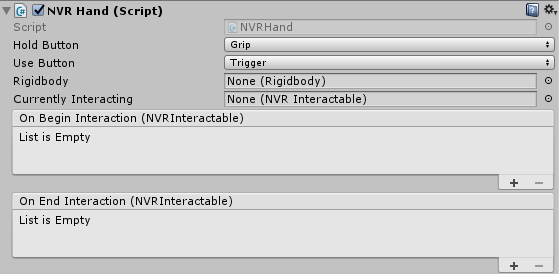
\includegraphics[width=\linewidth]{dissertation/newton_controller.png}
\caption{NewtonVR Controller Configuration System}
\end{subfigure}
\hfill
\begin{subfigure}[h]{0.21\linewidth}
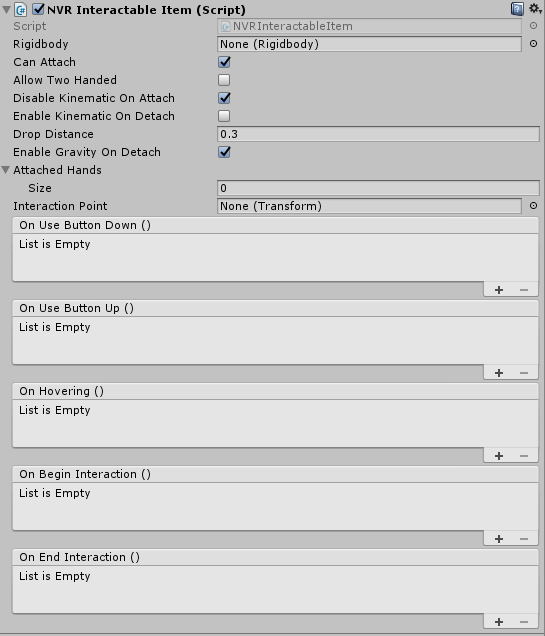
\includegraphics[width=\linewidth]{dissertation/newton_grab_object.png}
\caption{NewtonVR Event Bridge System}
\end{subfigure}
\hfill
\caption{Screenshots of the NewtonVR controller configuration and event bridge system}
\end{figure}

An event bridge system is included within the NewtonVR toolkit to allow the user to trigger some event upon performing some interaction (grabbing, interacting or hovering over an interactive object) within the application. This functionality is implemented directly into the ``Interactable'' script, which is the script used to make an object interactive within the application. Implementing this functionality directly into this script creates a cluttered interface that is often left empty as many objects need not make use of this functionality. This too is the approach taken by VRTK as discussed below. The SVRA approach to this is to instead abstracts the event bridge functionality out into a separate script as is discussed in Sections \ref{sec:decisiondesignoverview} and \ref{sec:decisiondesignarchitecture}. The problem of an overwhelming and verbose interface is seen throughout the NewtonVR toolkit and was highlighted by the clients of this project as one of the key critiques of the current toolkits on the market (Section \ref{sec:requirementsdndmeeting}). This was in addition to another complaint against the toolkit regarding of how difficult it was to learn to use. As only one example is provided with the toolkit which showcases all of the functionality at once and due to the associated documentation for the toolkit being extremely sparse and incomplete, a non-technical user attempting to learn to use the toolkit will struggle. Instead a toolkit aimed at non-technical developers in addition to providing a clean, concise, self-explanatory interface should also provide the user with a range of examples and resources for user training. This was shown to be especially true during the second round of evaluation (Section \ref{sec:evaluationround2}) where the majority of participants expressed that training resources and tutorials were as much of a necessity as a well designed, simple to use tool. 

\subsection{VRTK}
\label{sec:contextvrtk}
The Virtual Reality Toolkit\footnote{Developed by The Stonefox (\url{https://github.com/thestonefox/VRTK})} (VRTK) is a plugin for the Unity game engine that is designed to allows developers to rapidly build VR applications by providing a collection of scripts and Unity prefab objects. The toolkit includes an object interactive system, UI menus with interaction provided via a laser pointer system and a locomotion system including teleportation, touchpad movement and other non-traditional movement systems. The toolkit supports a wide variety of VR devices and contains a VR Simulator to allow developers to test VR applications without the need of VR device. The range of different device support is due to the implementation of an ``SDK Manager prefab'' which handles the setup of both the controllers and camera for the application. Unlike other toolkits, i.e. the NewtonVR toolkit, the SDK manager is not an all encompassing point of setup for the application, rather the controllers and camera must be setup independently of the SDK manager object. This increases the number of steps required in the setup and configuration of the toolkit for the targeted hardware platforms for development. Once setup it does allow for dynamic management and switching of the SDK in use but at the cost of the aforementioned more complex setup process. To reduce setup complexity an SDK manager such as this was omitted from the SVRA toolkit as discussed in Section \ref{sec:decisionnosdkmanager} though its potential as a beneficial feature in the long term is highlighted in Section \ref{sec:conclusionfuturework}.

The same critique made of the the NetwonVR controller configuration logic can also be made of VRTK's controller configuration logic. As with the NewtonVR method, VRTK also assigns buttons onto actions opposed to actions onto buttons. As stated above the reasoning for why the SVRA toolkit adopts the reverse logic is provided in Section \ref{sec:decisioncontrollersetup} and the discussion of the A/B Testing performed into the topic in Section \ref{sec:evaluationround2ab} where it was shown the user's preference was for the reversed logic used by the SVRA toolkit. An additional problem highlighted by the controller configuration system of VRTK but one that is seen throughout the toolkit is how more complex functionality and behaviour is added onto objects. For example, the default controller configuration and setup system allows users to map actions to buttons and to refine the sensitivity of the buttons. To extend the controller configuration to include a pointer system that is needed for teleportation, additional scripts must be added onto the object. This drastically increases the amount of options in the UI making it much more difficult to manage. This issue of adding more complex behaviour to an object through  attaching more scripts onto the object is also seen in VRTK's interactive object highlight system and the method by which connections are established between the controller and objects. The reasoning for this approach is likely to make the system more developer friendly where a developer can simply write their own custom script in place of one of the attached scripts to add the more complex behaviour. The consequence of this is increasing the complexity and density of the UI used by the user to configure the object which was addressed specifically by the client during the requirements meeting in Section \ref{sec:requirementsdndmeeting} where one of their biggest complaints against the toolkit was the verbosity of the UI. For a non-technical user requiring that they add multiple scripts where a single, self contained script could suffice is not user friendly. Instead, wherever possible, the user should be provided with a single script that encompasses all of the features within it. For example, where VRTK requires users attach different scripts onto an object to gain different types of object highlighting functionality the SVRA toolkit provides a highlighting through the selection of the highlighting method from a drop down menu and builds this functionality into every interactive object. This is discussed in full in Section \ref{sec:decisionhighlightingsystem}.

Where the NewtonVR toolkit failed to provide users with an extensive set of example scenes or documentation, VRTK provides users with an extensive and comprehensive set of examples, documentation and tutorials. Examples begin with the most basic of tasks of the toolkit and steadily increase in complexity, thus providing users with a structured, guided approach to learning the more challenging and complex features of the toolkit. Tutorial videos which guide users through the examples and their creation is also available alongside written documentation. The extensiveness of the provided training resources makes VRTK an attractive choice of toolkit for non-technical developers as it provides a clear road map to learn the features included in the toolkit starting from the most basic task and steadily increasing to the most complex tasks. The need for such a set of documentation and resources was highlighted during the second round of evaluation (Section \ref{sec:evaluationround2}) in particular.

\chapter{Requirements}
\label{sec:requirementschapter}
This chapter discusses the project requirements and the methods in which they were elicited. It identifies the functional and non-functional requirements of the project presented using the MoSCoW prioritization technique.

\section{Overview}
\label{sec:requirementsoverview}
The development of the SVRA project was requested by Dr. Julie Williamson (University of Glasgow). Dr. Williamson through working with artists from Dennis \& Debbie Club\footnote{\url{http://dennisanddebbie.club/}} to develop VR applications has firsthand knowledge of the challenges faced by non-technical developers whilst creating VR applications. Her envisioned application was the development of a VR development toolkit aimed at non-technical developers interested in creating VR content. It would provide a range of tools which could be used exclusively through graphical editing tools. 

The requirements for the project were identified through several individual meetings with Dr. Williamson and one including the aforementioned artists Debbie and Dennis. An initial set of requirements was given by Dr. Williamson during the two of the weekly supervisor meetings held with her at the offset of the project. During these meetings she highlighted several of the challenges faced by her and Dennis and Debbie (of Dennis \& Debbie club) during the development of the ``INTERN''\footnote{INTERN is a project made for the HTC Vive developed by Dr. Williamson and Dennis \& Debbie club} experience. This formed the basis of an initial draft of requirements and served as preparation for an interview with Debbie and Dennis to elicit additional requirements and gain a non-technical developers perspective and input. Both sets of requirements were then used to draft a final set of requirements for the project as discussed in Section \ref{sec:requirementsfunctionalnonfunctional}.

\subsection{Dr. Williamson Requirements Meetings}
\label{sec:requirementsdrwilliamson}
During two organised meetings at the offset of the project Dr. Williamson expanded on the goals of the project and outlined her vision for the application. In particular she highlighted the following key ideas. She reinforced the need to make the toolkit as non-technical developer as possible, \textit{``No coding required. Drag and drop this script here and you're set''}, with particular emphasis on minimising the number of clicks required for a given task and the required background technical knowledge of the user. Despite many of the existing toolkits advertising themselves as user friendly, her biggest complaint against them was they still require significant portions of technical knowledge to use effectively. Additionally such toolkits also require a lot of configuration and trial and error during development. From a non-technical developers perspective she expressed the benefits brought by the use of established defaults which provide a default setup for a particular object or interaction which can then easily modified by users via a GUI. She also highlighted some of the other challenges she encountered during her recent development experience such as transitioning between scenes\footnote{A Unity scene is a unique level in a game into which the user places the environment, objects and establishes all of the game logic}. Finally she suggested I consider the final state of the project and how it would be distributed to users. As the target users are non-technical developers the project should have as straightforward a setup process as possible. Platforms such as the Unity Asset Store\footnote{The Unity Asset store is a storefront for publicly created Unity extensions and assets} to provide a simple method by which users can install a custom extension to a game engine. As such it makes logical sense to target a release through this digital storefront as the method by which the tool could be most easily distributed to potential users. An extended summary of the points discussed here and her aims for the project can be found in Appendix \ref{sec:appendmreqmeetmins} which features extracts from the weekly meeting minutes documents produced throughout the development of the project which discuss the requirements and aims of the project.

\subsection{Debbie and Dennis Requirements Meeting}
\label{sec:requirementsdndmeeting}
Following the two requirements meetings with Dr. Williamson, a third meeting was organised to include artists Debbie and Dennis who would serve as the traditional ``client role'' for the project. Debbie and Dennis are two Glasgow based artists without a technical background whose work includes creating VR applications, CGI animations and video installations. Their lack of technical background provides an essential insight into the perspective of a non-technical developer and their problems with existing VR development toolkits.

The meeting itself took the form of an informal, semi-structured interview which served as a retrospective of the development of the ``INTERN'' project. Prior to the interview a set of draft questions were written, included for reference in Appendix \ref{sec:appendclientinterviewquestions}, based of my own background reading and the requirements provided by Dr. Williamson. This question set was not meant to be followed directly rather used as a basis for discussion points throughout the interview. The interview was recorded and later transcribed with additional notes and context into each of the topics discussed provided in post. The complete transcript is provided in Appendix \ref{sec:appenddndtranscript} with a summary of the interview and the key topics discussed outlined below. The interview began with Debbie and Dennis allowing me to experience the ``INTERN'' application. As I played through the ``INTERN'' experience they provided some insight into the development of the application as well as their original vision and any constraints they were forced to make during development due to the difficulties faced during development. This was followed by a code walkthrough of the source files as they outlined and discussed the challenges experienced during development. From this the following key topics were identified (presented in alphabetical order):

\textbf{Button Issues:}
A complaint of the client's against VRTK regarded the implementation of push buttons by the toolkit. Within the client's project they attempted to make a hand soap dispenser which the player would be able to pickup and then push a button the top of to dispense soap. In reality what occurred was that when the player picked up the object, moving the object up or down caused the button to constantly trigger as the object was being moved. Instead the client believed that rather than having a single, general button script that a class of buttons scripts would be more suitable. With a class of buttons, each button could be designed to suit some specific purpose, e.g. a wall button, a desk button, etc.

\textbf{Configuration Chains:}
One critique of VRTK was the amount of overhead and configuration required as part of the setup for more complex interactions. As complex interactions are setup, effectively what is built is a \textit{``configuration chain''} where should a single part of the setup be removed or misconfigured, the user is provided no way of knowing which part of the setup is missing or requires correcting. Instead, as suggested by the clients, what is needed is a more self-contained system which minimises the number of different components which require configuration. This in turn reduces the risk of bugs and errors and reduces the complexity of the system through reducing the number of different components to be simultaneously managed by the user.

\textbf{Event System:}
Both the NewtonVR toolkit and VRTK use an event system by which there is a method of triggering some event or function to occur based off some setup interaction caused by the player. The design and implementation of the VRTK event system was highly praised by the client being called ``basically perfect'' and was said to integrate into the Unity workflow very well. In particular it was praised for its simplicity, being intuitive to use and for allowing the user to easily see which events are setup to trigger under specified user interaction conditions. Due to the high praise given by the client to VRTK's event system the SVRA event system was modelled after the VRTK system. This is design of the SVRA event system is discussed in Section \ref{sec:decisiondesignoverview} and in Section \ref{sec:decisiondesignarchitecture}.

\textbf{Object Interaction System:}
One of the features of VRTK praised by the client was the options provided which allowed the user to specify how the player will pick up and interact with an object. For example when the player picks up an object you can force them to hold the object in a specified position at a specified orientation. Additionally, you can cause the player's controller model to disappear upon picking up an object. As such the SVRA toolkit chose to implement such positioning and orientation directly into the object interaction system as is discussed in Section  \ref{sec:decisionobjectinteractiondesign}.

\textbf{Overwhelming Interfaces \& Configuration Options:}
A major point of complaint of the clients against VRTK was the overwhelming number of options provided on the UI for customising scripts attached onto objects. They felt this was especially true for simple objects and interactions where the corresponding UI and configuration options are overwhelmingly dense. For something as simple as a drawer the client commented \textit{''A lot of these [configuration options] are not necessary because it’s just a drawer. It's not a lightsaber you can click on or something.``}. A second related critique regarding the configuration options of scripts was the counter intuitiveness of the text for the configuration options themselves. As an example the client selected the option to enable an object to be picked up or not, \textit{``Does 'is usable' mean use only when grabbed or hold a button to use?''}. Instead the client suggested that a reduced number of options and a clearer, more self explanatory interface would vastly increase the usability of the system. 

\textbf{Scene Transition Problems:}
One of the more challenging, frustrating and time consuming parts of the development was attempting to implement a custom loading screen for the transition between Unity scenes. A Unity scene can be thought of as a unique level in a game into which the user places the environment, objects and establishes all of the game logic. Scene transitions are extremely common and transitioning from one created scene to another should be as the client said ``trivial'', opposed to the opposite experience which was found by the client. This was, as discovered by the client, partly due to the SteamVR plugin for Unity which features hard coded values and stub methods which resulted in unexpected behaviour. Instead what is desired by the client is a scene transition system with drag and drop options to customise the transitioning space, the compositor transition scene. The compositor transition scene is a scene used by the SteamVR plugin to transition between Unity scenes whilst maintaining a steady framerate during the loading of the next scene to ensure the player does not feel motion sick due to a unsteady framerate during the scene transition and loading. Customisation options for this transition space would include a drag and drop method of easily setting up the surrounding background, floor, etc. of the space.

\textbf{Script Attachment System:}
One of the client's major complaints regarding the usability of VRTK concerned the need to add more scripts onto the controller objects to get access to additional functionality. This was discussed in Section \ref{sec:contextvrtk} where it was noted that a similar system exists for object highlighting where additional highlighting scripts are attached onto objects to override the basic highlighting system provided to all interactive objects. Aside from the usability decrease to UI, the client expressed that this approach is quite difficult to learn and to manage due to the amount of possible combinations present within the toolkit, \textit{``Things get very complicated very quickly''}.

\textbf{Spectator Settings Configuration:}
One of the client's key aims for the project was to change the controller model seen by a spectator of the application being experienced. That is the player would see the HTC Vive controller within the application but the spectator watching the player would see a hand in place of the controller. Aesthetic changes such as this are of interest to the client and being able to easily modify a spectator's view of the experience by for example showing alternative camera viewpoints and perspectives, changing the model of the controller and headset, etc. was discussed during the meeting.

\textbf{Testing Complaints:}
One of the most time consuming aspects of development is the testing of the application something that is especially true in VR development. To test a VR application, the developer must transition from working on the development machine to putting on the VR hardware, entering the application and then testing the change made to the application. This back and forth is extremely tiresome for a single developer and the best approach found by the clients during the development was to have at one person wearing the hardware constantly to test the application and one person working at the development machine making the changes to the application. This is not a feasible solution for smaller development teams and so some form of testing automation would greatly reduce the time consuming and tiresome nature of testing VR applications. Alternatively method of altering the application from within would also assist with the development process by allowing changes to be made from within the application rather than being required to be made from the development machine. 

\section{Functional \& Non-Functional Requirements}
\label{sec:requirementsfunctionalnonfunctional}
Due to the open ended nature of the original specification there were various potential directions for the development of the project. The various requirements interviews resulted in a wide variety of potential features which were then analysed and a subset of the core, key features was selected as the functional requirements for the project. This was done by first grouping the different potential features into categories, in a lightweight version of open, axial and selective coding \cite{openaxebook} and then deriving some casual use cases \cite{usecases} for each category of feature. Included in Appendix \ref{sec:appendreqcat} is a document produced during the catergorisation of the different types of requirement suggested for the project during the various requirements meetings held. These were then prioritised using the MoSCoW prioritization technique. A set of non-functional requirements for the project was also identified. Both sets of requirements were drafted as a means of ensuring the project matched the original intent of Dr. Williamson’s envisioned application. However, room was left for feature discovery within the requirements as due to the aforementioned open nature of the project it was likely new potential features would arise throughout development whose inclusion would be beneficial to the product and might take priority over some of the previously proposed features.

\subsection{Functional Requirements}
\label{sec:requirementsfunctional}
The functional requirements of a product describe how the application should behave in order to support the user goals and activities. The functional requirements of the product were structured in terms of priority using the MoSCoW method \cite{moscow} which categorises requirements into four priorities: ``Must Have'', ``Should Have'', ``Could Have'', ``Won’t Have'', with the requirements in each category being unordered as it is likely requirements within the same category are of the same importance, hence they are presented alphabetically in the following tables. 

The requirements included in Tables \ref{tab:musthave}, \ref{tab:shouldhave}, \ref{tab:couldhave}, \ref{tab:willnothave}, overleaf, represent functionality that the application broken down into the four MoSCoW priorities. The four tables provide a general overview of the different components required for the product to be deemed ``feature complete'', a more in depth set of MoSCoW tables was produced during the requirements gathering phase of the project, included for reference in Appendix \ref{sec:appendmoscow}. These provided a more detailed breakdown of what it meant for each of the components to be deemed as ``feature complete'' for the project.

\begin{table}[]
    \centering
    \begin{tabular}{ | p{5.5cm} | p{10.5cm} |}
        \hline
        Requirement & Description \\ \hline
        Button Class System & The product contains options for different forms of buttons which allow the user easily setup a button within the application that triggers some event upon the user pressing the button \\ \hline
        Controller Configuration System & The product allows the user to configure the controls of their controller and easily change the model and visibility of the controller within the game \\ \hline
        Grabbable Object Interaction System & The product contains an object interaction system that allows users to easily setup grabbable objects within the application \\ \hline
        Intuitive GUI Interface & The product is used through an intuitive, GUI interface and does not require the user to write code to implement their application \\ \hline
        Movement (Teleportation) System & The product contains a locomotion system by which the user can easily setup so that they are able to move within their application \\ \hline
        Object Default Setup: Drawers \& Cupboards & The product contains a default configuration for common items such as drawers and cupboards for users to use \\ \hline
        Scene Transition System & The product contains a method by which to easily transition from one Unity scene to the other \\ \hline
    \end{tabular}
    \caption{Must Have Requirements Table}
    \label{tab:musthave}
\end{table}

\begin{table}[]
    \centering
    \begin{tabular}{| p{5.5cm} | p{10.5cm} |}
        \hline
            Requirement & Description \\ \hline
            Automated Testing System & The product contains an automated test system by which users can run “unit test like” tests on their application so that the application functionality may be tested without the developer needing to use the VR hardware to test the application \\ \hline
            Controller Configuration & The controller configuration system is extended to include a set of custom buttons established on the touchpad of the HTC Vive controller and additional cosmetic options to customise the controller’s appearance in-game \\ \hline
            Object Default Setup: Doors \& Leavers & The product contains a default configuration for common items such as doors and leavers for users to use \\ \hline
            Object Interaction System (Sound Collision Framework) & The object interaction system within the product is extended to include a sound collision framework that allows users to easily setup audio cues associated with different interactive objects \\ \hline
    \end{tabular}
    \caption{Should Have Requirements Table}
    \label{tab:shouldhave}
\end{table}

\begin{table}[]
    \centering
    \begin{tabular}{ | p{5.5cm} | p{10.5cm} |}
        \hline
        Requirement & Description \\ \hline
        Controller Physicality Option & The product contains the functionality allowing the a user’s controller to be made into a physical object which can interact with other interactive objects within the application \\ \hline
        Event-System Finite State Machine & The product contains a (predeveloped) Unity finite state machine which contains an intuitive interface for users \\ \hline
        Object Default Setup: Boxes \& Chests & The product contains a default configuration for common items such as boxes and chests for users to use \\ \hline
        Object Interaction System (Highlighting) & The object interaction system within the product is extended to include a highlighting system which highlights interactive objects to users when they hover their controller over the object \\ \hline
    \end{tabular}
    \caption{Could Have Requirements Table}
    \label{tab:couldhave}
\end{table}

\begin{table}[]
    \centering
    \begin{tabular}{ | p{5.5cm} | p{10.5cm} |}
        \hline
        Requirement & Description \\ \hline
        Additional VR Hardware Support & The product supports additional hardware platforms beyond the HTC Vive such as the Oculus Rift, Samsung Gear VR, etc. \\ \hline
    \end{tabular}
    \caption{Will Not Have Requirements Table}
    \label{tab:willnothave}
\end{table}

\newpage
While this was the initially produced set of functional requirements due to the effect of feature discovery and change of requirements throughout the project's development not all of the proposed requirements were implemented into the project. Instead time was spent of newly discovered features which were deemed more significant to the success of the project. While some features remain highly desirable and are excellent sources of future feature development (Section \ref{sec:conclusionextendingtoolkit}) others such as the ability to change the model of the controllers and HMD were found to not be as significant as originally estimated. This was due to the functionality to do this being included in a straightforward manner by the SteamVR SDK and were estimated as being more difficult due to my own inexperience with the SteamVR SDK at the time of writing the requirements.

\subsection{Non-Functional Requirements}
\label{sec:requirementsnonfunctional}
The non-functional requirements are concerned with the application users and their ability to effectively use the product and describe how well a system performs its goals. The non-functional requirements which were identified for the product are listed below: 

\begin{table}[h]
    \centering
    \begin{tabular}{ | p{5.5cm} | p{10.5cm} |}
        \hline
        Requirement & Description \\ \hline
        Code Free Experience & The product will provide a code free experience with the user not being required to touch any piece of code during the creation of their intended application \\ \hline
        Consistent Interactions & Objects and interactions will work consistently across different types of Unity environments and setups and will not be limited to some predefined set of restrictions \\ \hline
        Easily Modifiable Settings & Objects which default to some predefined setting will be easily modified and customised by the user via an intuitive GUI \\ \hline
        Minimal Number of Clicks & The user’s task will be accomplished with the minimal number of clicks relative to the task being performed \\ \hline
        Minimal User Setup \& Repetition & The toolkit will minimise the amount of setup, configuration and repetition required of user’s whilst using the toolkit \\ \hline
        Pre-Established Defaults & Default version of interactive objects will be created wherever possible. Scripts which setup objects as interactive and controllers will default to some predefined default setting \\ \hline
        Straightforward Feature Addition & Technical users should be able to easily and quickly incorporate new functionality and features into the toolkit without disrupting the existing feature set \\ \hline
        Straightforward Feature Customisation & Technical users should be able to easily modify an existing feature to their particular need \\ \hline
    \end{tabular}
    \caption{Non-Functional Requirements Table}
    \label{tab:nonfunc}
\end{table}

\chapter{Design}
This chapters provides a overview of the design of the toolkit. It discusses the preliminary decisions which were made prior to development beginning on the toolkit as well as the usability and the technical design decisions made during the development of the system. 

\section{Preliminary Design Decisions}
Prior to discussing the usability and technical design decisions made it is worth first discussing the rationale behind the preliminary design decisions made. That is the choice of game engine for which the toolkit would be built and the choice of hardware device for development. Finally the decision on whether to build an entirely new toolkit opposed of simplifying an existing toolkit is also discussed.

\subsection{Choice of Game Engine}
\label{sec:decisionunity}
As discussed previously in Section \ref{sec:contextgameengines} a game engine allows developers to reuse components across different projects to help to streamline the development process. Of the popular game engines on the market the Unreal Engine 4 and Unity platform were considered for this project with the Unity game engine being selected as the game engine for which this project was to be built. Using the Unity platform developers are able to create complex environments using a graphical user interface and so it is suitable for the needs of a non-technical user. From a developer standpoint, the Unity platform is very easily extended through custom tools which can be easily built and distributed to users through services such as the Unity Asset Store. Where the Unity platform falls short is that many more of its advanced features, those included in the SteamVR SDK for example, are difficult to implement without extensive programming experience. However, this is the goal of the SVRA toolkit which aims to create a range of tools which can be used exclusively through the Unity graphical editing tools. From a user-base perspective the Unity platform, being the market leading consumer game engine, is the most sensible platform to target. With a VisionMobile survey \cite{VisionMobile} showing that 59\% of virtual reality developers are using the Unity platform, the Unity platform has both the dominant market of VR and non-VR developers. Additionally whereas the Unreal Engine documentation is lacking, especially in regards to its technical documentation, the Unity documentation is much more thorough and complete. The Unity platform, due to its greater install base, also has a greater variety of tutorials and training resources for a new developer. As such it is the clear choice of game engine for this project. 

\subsection{Choice of Target Platform}
\label{sec:decisionhardware}
Due to the time constraints enforced on the project the decision was made at the start of development to target a single hardware platform for release. Despite existing toolkits supporting both the HTC Vive and Oculus family of devices, amongst others, due to the time constraints it was decided that by targeting a single platform for release a more in-depth feature set for that particular device could be provided. By choosing to build the toolkit on multiple platforms it was likely that a smaller feature set would be implemented across multiple devices due to the additional time required for development and testing of the toolkit on multiple pieces of hardware simultaneously. This reduced feature set risked several of the aims of the SVRA toolkit not being met due to the additional overheads introduced into the development pipeline by targeting multiple platforms for release. Instead the decision was made to select a lead hardware platform for development and then to port the toolkit to additional platforms at a later date if it proved successful on release. This practice of porting software is common throughout the software industry, especially within the video game industry where developers typically build for the PC and then later port the game to the console platforms.

Of the two leading devices on the market, the Oculus family of devices and the HTC Vive, the HTC Vive was selected as the lead platform for development. Aside from being a platform in which the clients all had joint background experience with their recent development of the ``INTERN'' application, the HTC Vive as was recently highlighted by a 2018 industry survey by the Game Developers Conference \cite{gdcsurvey} is the leading device amongst developers. This is a trend that was seen in the previous years survey as well where the HTC Vive overtook the Oculus Rift as most popular device among developers. Although it remains the narrow leader with 15\% of respondents releasing their previous game on and 17\% stating they were currently working on a game to be released for the HTC Vive, compared to the 14\% and 16\% seen on the Oculus Rift, developer interest in the platform remains high. 33\% of developers state they are most interested in the HTC Vive platform opposed the the 20\% seen by the Oculus Rift. The same survey also states that the both the VR technology developers, the developers creating tools to create VR applications, and the VR content creators, the developers creating VR applications, believe that the HTC Vive is the best quality tethered HMD experience. This is in addition to the HTC Vive being voted as the best rated HMD for quality of experience. As the HTC Vive is the, albeit narrow, leading device on the market for both developers and content creators in addition to being the device in which the clients had the most recent development experience, it is the obvious choice of lead development platform for this project.

\subsection{New Toolkit or Extension to Existing Toolkit}
\label{sec:decisionnewtoolkit}
With the selection of game engine and hardware platform decided the next decision to be made concerned the nature of the toolkit itself. Should the development build an entirely new toolkit or should instead the toolkit be and extension to an existing toolkit to simplify its use? The potential for an extension to be made to an existing toolkit is discussed in Section \ref{sec:evaluationround3} and in Section \ref{sec:conclusionproofofconcept} with the decision being made to start development of a new toolkit for this project. Although this decision was primarily made to allow for complete creative control over the design and direction of the product other benefits did also factored into the decision. Most significant was to ensure that the toolkit was not reliant on other existing toolkits which are suspect to change or risk halting development and becoming obsolete. This too is discussed in Section \ref{sec:conclusionproofofconcept} but the time saved by simplifying the use of the features of an existing toolkit was not deemed as enough justification not to build the system from the ground up to account for the needs of a non-technical developer. Ultimately this decision proved to be the correct one as the likely chosen existing toolkit to simplify would be VRTK but at the start of 2018 the solo, lead developer of VRTK announced that his involvement with the project was over. With this the VRTK project was left as open source software and as of March 2018 has had significant additions or changes made by the community to the project. 

\section{Toolkit Design Decisions}
\label{sec:decisiontoolkitdecisions}
The remaining design decisions discussed in this chapter concern the design of the usability of the toolkit and the technical decisions made during the development. This section is concerned with the usability design of the product and provides the rationale behind the key design decisions made.

\subsection{Design Overview}
\label{sec:decisiondesignoverview}
The philosophy of the SVRA toolkit's design is to reduce the complexity of making VR applications and to minimise the number of steps required to perform common development tasks. To achieve this the toolkit attempts to make the process of creating an application as intuitive as possible. First users must setup the camera and controller before setting up the interactions within the application. This is achieved in the SVRA toolkit by importing the necessary SteamVR camera and controller prefabs and attaching the SVRA controller configuration prefab onto the controllers. This setup the controllers with a default control scheme and users can to easily reconfigure the buttons of the controller by mapping actions, such as ``grab'' or ``interact'', onto the buttons of the controller. Additional configuration settings for the controller such as altering the collision detection radius for objects are configured here as well. 

Making objects ``grabbable'', that is they can be picked up by the player with a ``grab'' action assuming the controller is setup, requires only adding the ``grabbable object'' script onto the object to be made grabbable. Specifics regarding how the object should be picked up, its position and orientation, and the highlighting effect to occur when the controller is within the collision detection radius are configured through this script's attributes in the Unity Inspector window\footnote{The Unity Inspector window displays detailed information about the currently selected object within the Unity scene and allows the user to modify the attributes and behaviours of the scripts attached to the object} Making objects ``interactive'', meaning they can be interacted with by an ``interact'' operation works similarly in that users need only add the ``interactive object'' script onto the object and setup the controller. In order to trigger some function or event occurring upon an interaction event (grabbing, interacting with or touching an object) users must add an ``event bridge'' onto the triggering interaction and a connection made between the triggering object and the triggered event. 

Controller configuration, the grab and interact actions and the event bridge form the core of the SVRA toolkit with a significant portion of the remaining features seen in the toolkit being sample, default interactions which make use of the event bridge to perform some common event. Examples of such sample events include switching between Unity scenes, disabling the ability to interact with or grab an object and the ability to change the colour or material of an object. The details of the implementation of the toolkit are discussed in Section \ref{sec:implementationchapter} and the system architecture employed in Section \ref{sec:decisiondesignarchitecture}. Several tools to assist with the debugging of applications are included in the toolkit. An active frame rate detector provides a active display of the current frame rate of the application through the HMD and a camera modifier allows users to scale, rotate and move the world dynamically whilst within the application using the keyboard. The implementation of both features is discussed in Section \ref{sec:implementationdebuggingtoolkit}.

\subsection{Lack of SDK Manager}
\label{sec:decisionnosdkmanager}
One of the first decisions to be made concerned how users would setup the controllers and camera for the application. Where the VRTK and NewtonVR toolkits provide some form of SDK management system, the SVRA toolkit omits this in favour of setting up the SteamVR SDK\footnote{The SteamVR SDK is a Unity plugin for working with the HTC Vive device} camera and controller prefabs directly. The decision to take this approach was made to minimise the number of steps required in the setup of the toolkit as the SDK managers often have you establish which hardware device you are working as part of their more complex setup process. Instead the SVRA toolkit only requires the user add the SVRA ``ControllerSetup'' prefab onto each of the SteamVR controller prefabs and then assign the tracked controller attribute to be the left and right controller respectively. The use of configuring the SteamVR prefabs directly allows users to make use of the multitude of existing documentation, tutorials and resources for working with the SteamVR prefabs rather than rely solely on the documentation and tutorials produced for the SVRA toolkit. Finally as development chose to target one platform it was decided that a better use of development resources was to not spend time working on an unused SDK manageement system but rather on prototyping and implementing more functionality into the toolkit. The potential of an SDK management system does exist though as is discussed in Section \ref{sec:conclusionfuturework}.

\subsection{Controller Setup Logic}
\label{sec:decisioncontrollersetup}
Both the VRTK and NewtonVR toolkits configure the controllers by asking the user to assign buttons onto the possible actions of the toolkit. For example, the NewtonVR toolkit consists only of two actions ``hold'' and ``use'' onto which the players assign the buttons of the controller to cause the respective action. This approach does not scale should the list of possible actions increase greatly as the toolkit develops over time and more actions are added. 

\begin{figure}[h]
\begin{subfigure}[h]{0.3\linewidth}
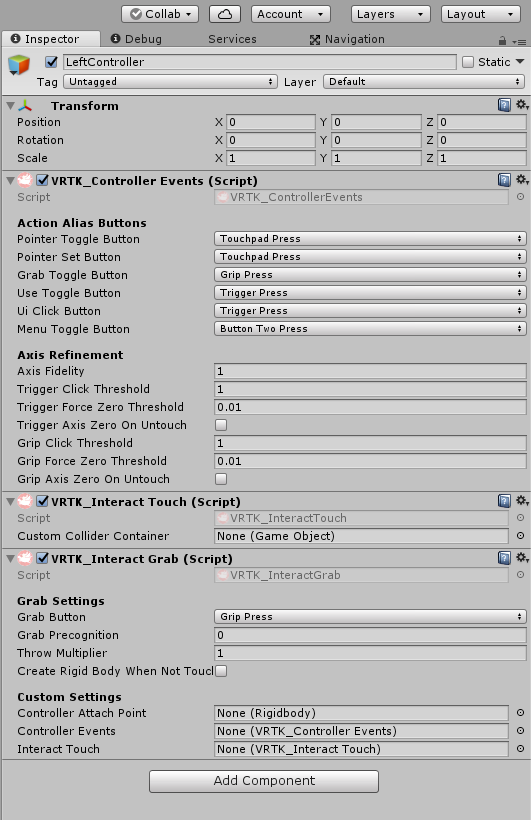
\includegraphics[width=\linewidth]{dissertation/vrtk_controller_setup.png}
\caption{VRTK}
\end{subfigure}
\hfill
\begin{subfigure}[h]{0.3\linewidth}
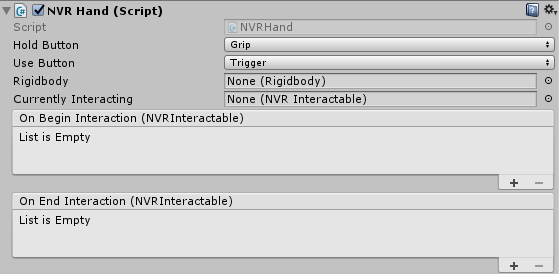
\includegraphics[width=\linewidth]{dissertation/newton_controller.png}
\caption{NewtonVR}
\end{subfigure}
\hfill
\begin{subfigure}[h]{0.3\linewidth}
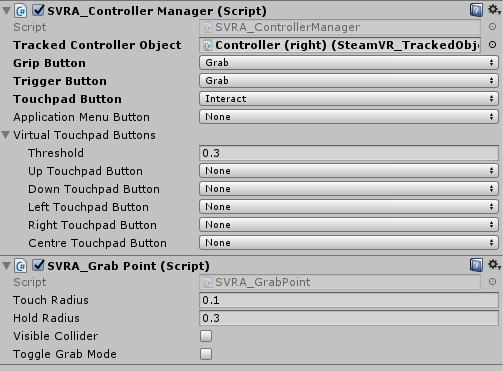
\includegraphics[width=\linewidth]{dissertation/svra_controller.png}
\caption{SVRA}
\end{subfigure}
\caption{Comparison of the interfaces for controller configuration}
\end{figure}

The above graphics highlight the difference in controller configuration methods used by the VRTK, NewtonVR and SVRA toolkits. As shown the SVRA toolkit adopts the reverse logic, where users specify the action to be associated with the button on the controller. In this system users are presented with a list of the buttons on the controller and must assign the action to occur when the button is pressed. Buttons which are reserved, such as the HTC Vive ``System Button'' and cannot be overwritten by a developer are omitted from the button list. Furthermore a set of 5 virtual buttons are implemented on the HTC Vive's touchpad (up, down, left, right, centre) to artificially increase the number of buttons from 4 to 8. Intuitively it was believed that this system falls more inline with the user's expectation. To confirm this hypothesis a round of A/B testing was performed where users were asked to experience both logic systems during the evaluation process and asked to select and justify their preference. The full discussion is contained in Section \ref{sec:evaluationround2ab} but it was found that the majority of users favoured the reverse logic approach adopted by the SVRA toolkit.

\subsection{Object Interaction System}
\label{sec:decisionobjectinteractiondesign}
One of the most fundamental decisions to be made concerned how the object interaction system would be designed in the SVRA toolkit. This design of the interaction system required several key decisions be made. First how the user would setup an object to make it ``grabbable'' (the player can pick up the object) and how the user would make an object ``interactive'' (the player can interact and use the object). Where VRTK uses a general ``interactable object'' script to represent both interactive and grabbable objects, the decision was made instead to implement two separate scripts to achieve this functionality. This decision was made based on the client’s comments that the single script cannot not intuitively express the intention of both actions and instead they should be separated into two distinct scripts. Consequentially as a result of making two distinct scripts the configuration UI for each script will reduce in verbosity.  

The next decision regarding the interaction of objects concerned how to implement the positioning and orientation functionality as is provided by VRTK. VRTK achieves this functionality by attaching specific scripts onto the object to modify how the player will interact with the object. The SVRA toolkits approach attempts to provide the same functionality but includes it within the grabbable object script. In the SVRA toolkit users can position and orient how the player will pickup the object by default from the grabbable object script. While more limited it is believed that this approach is better suited for non-technical developers as it reduces the complexity of the UI and removes the to attach and manage different scripts to an object for custom positioning and orientation upon pickup. The limitation of this system was discussed during the third round of system evaluation and is included in full in Section \ref{sec:evaluationround3}.

\begin{figure}[h]
\begin{subfigure}[h]{0.3\linewidth}
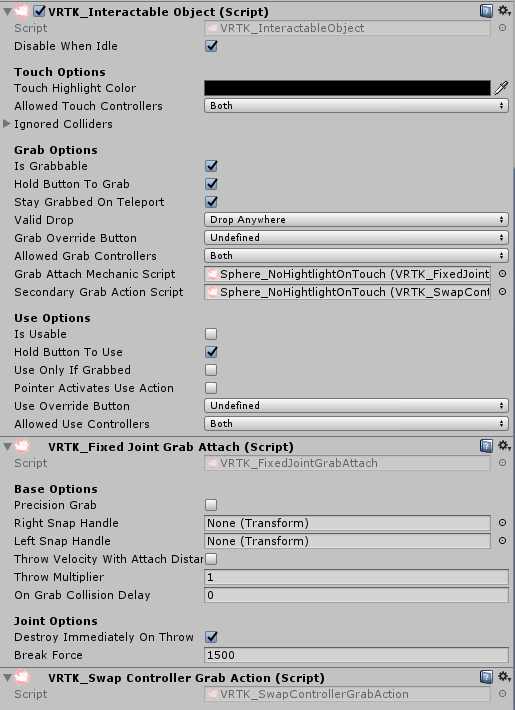
\includegraphics[width=\linewidth]{dissertation/vrtk_object.png}
\caption{VRTK}
\end{subfigure}
\hfill
\begin{subfigure}[h]{0.3\linewidth}
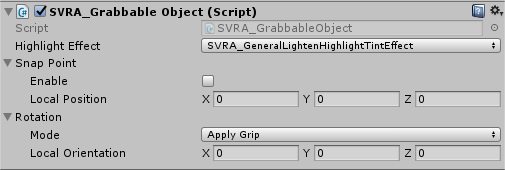
\includegraphics[width=\linewidth]{dissertation/svra_grab_object.png}
\caption{SVRA}
\end{subfigure}
\caption{Comparison of the interfaces for grabbable objects}
\end{figure}

A comparison of the interfaces presented by the SVRA toolkit and the VRTK equivalent for interacting with grabbable objects is presented above. The final decision regarding object interaction concerned how the connection would be established between the object and the controller. For this decision it was decided to perform background research into the interaction systems employed by various popular VR applications, specifically the video games Job Simulator\footnote{Developed by Owlchemy Labs}, Budget Cuts\footnote{Developed by Neat Corporation} and The Lab\footnote{Developed by Valve Corporation}. Although slight variations exist between the applications, the most common system employed is one in which the connection between the controller and the object breaks after some threshold force or distance is reached. That is if the player were to pick up an object and push it into an immovable object after some threshold distance of separation between the controller and the object the connection between the two would break and the object automatically dropped. 

With this design in mind two prototypes were created. The first established the connection using the native Unity joint system, the method by which one rigidbody object attaches to another or to a fixed point in space, and default physics system. The second was modelled after the NewtonVR approach and implemented a custom physics system on top of the native Unity joint system. Despite the latter system providing an improved physics effects it was found to introduce bugs to the positioning and orientation systems within the object interaction system. This was due to the added complexity introduced by the custom physics system and so the first prototype was selected as the chosen method and its implementation is discussed in Section \ref{sec:implementationcontrollerconfiguration}. An improved controller-object interaction system with an improved physics system remains a feature worth pursing as discussed in Section \ref{sec:conclusionextendingtoolkit}. 

\subsection{Object Highlighting System}
\label{sec:decisionhighlightingsystem}
Highlighting interactive objects when the controller is within the radius where an interaction can occur is a very frequent effect seen in VR applications. VRTK implements a general object highlighting system directly into its ``Interactable'' object script with more complex forms of highlighting  established by attaching different highlighting scripts onto the object to override the default highlighting system behaviour. As previously discussed in Section \ref{sec:contextvrtk}, VRTK's method of extending functionality by attaching additional scripts to an object introduces complexity due to the need to manage multiple scripts simultaneously and from the increase in UI verbosity. Instead the system should provide a single point of setup where users specified the highlighting effect to be used and then provide additional configuration if necessary. This is the approach adopted by the SVRA toolkit which builds highlighting directly into all interactive and grabbable objects. The highlighting effect is then selected from a drop down list of the different highlighting effects included in the toolkit. This approach provides the same functionality as the VRTK method but eliminates the need to manage multiple attached scripts to setup highlighting and greatly reduces the complexity of the UI. A comparison of the approaches used by the VRTK and SVRA toolkits is provided below. The VRTK method has a separate script attached to the object in addition to the ``Interactable'' script. An example of such a script is shown below.The SVRA method instead uses the selection of the highlighting effect script from a drop down list of scripts which is built directly into the interactive object scripts rather than requiring the user attach multiple scripts to the object.

\begin{figure}[h]
\begin{subfigure}[h]{0.4\linewidth}
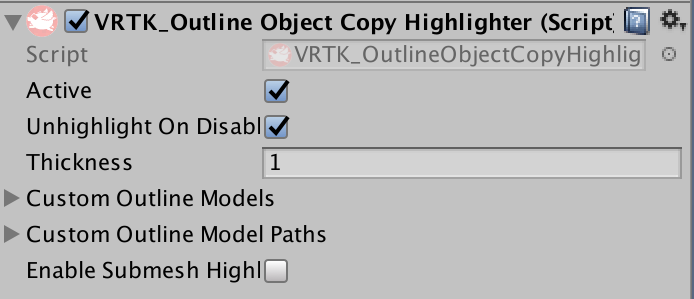
\includegraphics[width=\linewidth]{dissertation/vrtk-highlight.png}
\caption{VRTK}
\end{subfigure}
\hfill
\begin{subfigure}[h]{0.4\linewidth}
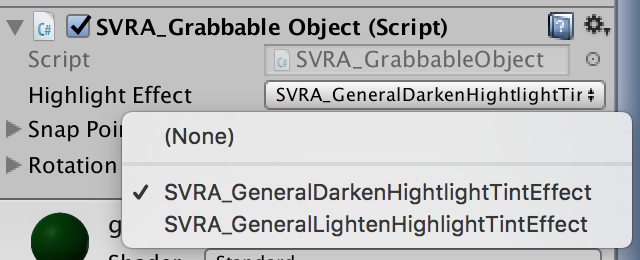
\includegraphics[width=\linewidth]{dissertation/svra-highlight.png}
\caption{SVRA}
\end{subfigure}
\caption{Comparison of the highlighting systems}
\end{figure}

\subsection{Lack of Custom Editor Windows}
\label{sec:designnoeditorwindows}
One of the key decisions to be made within the project was regarded whether it was worth the development resources to spend time making custom Unity editor windows for the product. The Unity Inspector window displays detailed information about the currently selected object within the Unity scene and allows the user to modify the attributes and behaviours of scripts attached to an object. Developers may extend the Inspector window and provide a custom interface to simplify the editor windows which can become cluttered when a lot of scripts are attached to the same object. To assist with the decision of if it was justifiable to spend the development resources on such a feature two prototypes custom editor windows were created. One was a custom window for altering a script attached to an object whereas the other was a custom interface for the Inspector window for interacting with the same script. This round of prototyping provided a much needed insight into the creation process behind custom window and Inspector interface development within Unity and it was decided that it would not be worth the additional time needed to implement such interfaces. This topic is discussed again during the expert evaluation of the project, in Section \ref{sec:evaluationround3}, where the use of custom windows was suggested for the project but only at the end of the feature's development and if deemed absolutely necessary due to the time consuming nature of their development. 

\section{Technical Design Decisions}
The final design decision discussed concerns the system architecture which was used in the implementation of the system. 

\subsection{Architecture Design}
\label{sec:decisiondesignarchitecture}
The key components of the system architecture are the use of the observer design pattern in the controller-object interaction system and the event bridge that is used to trigger a function call upon some interaction event occurring. The observer design pattern \cite{observer} is a software design pattern in which a subject object maintains a list of its dependents, called observers, and notifies them automatically when any state changes. Typically used in event handling systems, the observer pattern was identified as being suited for use here due to the controller-object relationship used for object interaction. The controller, the subject, broadcasts interaction messages to the dependents, the list of potential interactive objects within the collision radius of the controller, upon specified actions occurring. This broadcast results in some event occurring between the controller and the objects within its collision radius. For example, when the controller hovers over an interactive object a touching and highlighting message are broadcast to signify to the object it may be interacted with and in order to setup any highlighting effects that are in place on the object. Provided the object contains the grabbable script, should the player choose to grab the object then a grab message is broadcast which is signals that a grab connection should be established between the controller and the object thus creating the joint connection between the controller and object. 

\begin{figure}[h]
\begin{subfigure}[h]{0.4\linewidth}
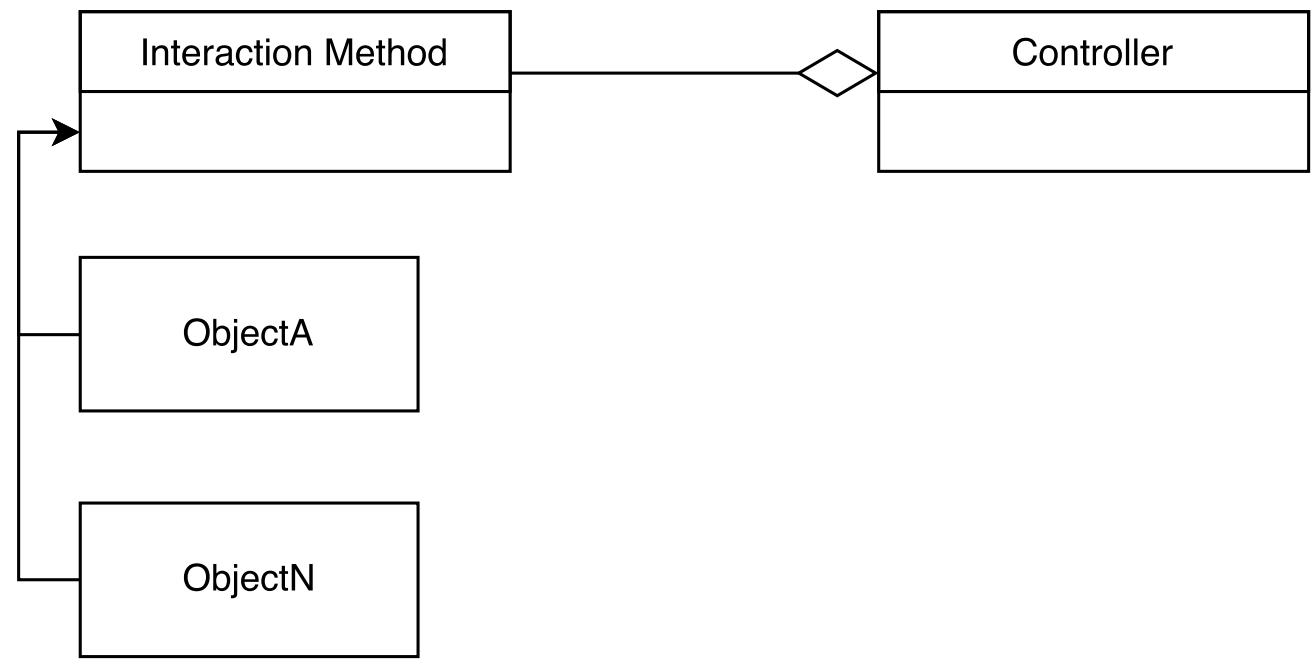
\includegraphics[width=\linewidth]{dissertation/observer.png}
\caption{Controller-Observer}
\end{subfigure}
\hfill
\begin{subfigure}[h]{0.4\linewidth}
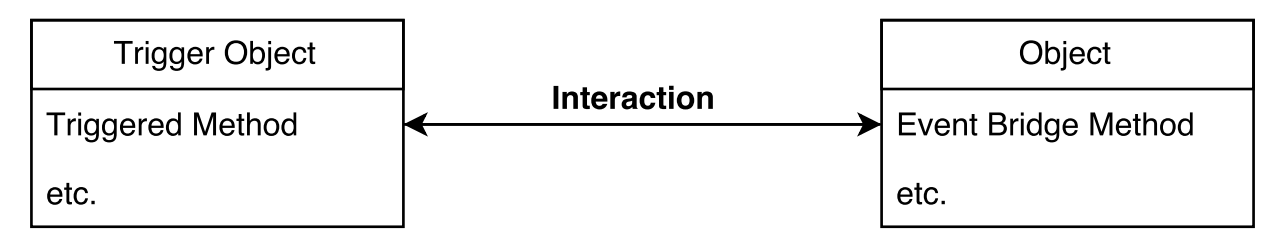
\includegraphics[width=\linewidth]{dissertation/event.png}
\caption{Event Bridge}
\end{subfigure}
\caption{System diagrams for the controller-observer and event bridge}
\end{figure}

The event system, termed the event bridge, employed within the toolkit is designed to allow function calls to occur upon some interaction event occurring. For example, a colour change of an object can be trigger on either grabbing,  touching, highlighting or interacting with some object. The event bridge system is abstracted into its own unique script in contrast to the VRTK system which is embedded into all interactive objects. While the approach adopted by the SVRA toolkit does contain some problems, as discussed in Section \ref{sec:evaluationround3}, it does provide a concise mechanism by which interaction events can trigger some function to occur. 

\chapter{Implementation}
\label{sec:implementationchapter}
This chapter provides details on the implementation of the product. It first discusses the implementation of the three key components of the product: the controller configuration system, the controller-object interaction system and the event bridge system. It then discusses the implementation of the various sample interaction scripts and debugging tools provided within the toolkit. All of the implementation was done using the C\# programming language as is required by the Unity platform.

\section{Controller Configuration \& Object Interaction}
\label{sec:implementationcontrollerconfiguration}
As outlined in Section \ref{sec:decisiondesignoverview} the controller configuration system forms one of the three core features of the toolkit. Controller configuration is handled by a controller setup prefab, \texttt{ControllerSetup}, which is attached to each of the controller prefabs provided by SteamVR. The prefab is built from two classes: \texttt{SVRA\_GrabPoint} and \texttt{SVRA\_ControllerManager} both of which form the part of the core of the toolkit's object interaction system. The buttons are assigned actions via the Inspector window as outlined in Section \ref{sec:decisioncontrollersetup} with the \texttt{SVRA\_ControllerManager} class using a dictionary to keep a record of which actions are assigned to each button. This dictionary is setup when the application is run. This class is also responsible for checking the state of each button on the controller, via its \texttt{Pressed}, \texttt{Released} and \texttt{Held} methods, which check if any button is currently being pressed, has been released or is being held down and return an enum stating which action is mapped to the button and should be performed.

The \texttt{SVRA\_GrabPoint} class is used to broadcast messages should the controller perform an action to be broadcast (the \texttt{BroadcastTouch}, \texttt{BroadcastGrab} and \texttt{BroadcastGrab} methods). It constantly monitors if the controller is performing an action and checks if an object is  currently being held by the controller. This check is performed by calling the \texttt{HoldingSomething} method of the \texttt{SVRA\_GrabConnection} class to check if an object is currently attached to a controller. When a held object is released the \texttt{DestroyConnection} method of the \texttt{SVRA\_GrabPoint} class sends a message to break the connection between the controller and the object. Additional attributes of the \texttt{SVRA\_GrabPoint} class include two boolean variables, \texttt{toggleGrabMode} and \texttt{visibleCollider}. Setting the \texttt{visibleCollider} variable to true within the Inspector window causes a sphere to be drawn showing the collision detection area for which if an interactive object enters then the controller can interact with it. The radius of this collision detection sphere is also modified here using the \texttt{touchRadius} attribute of the \texttt{SVRA\_GrabPoint} class. The \texttt{toggleGrabMode} variable if set to true switches the grab action logic from requiring the user to hold down the grab button on the controller to keep hold of the object to requiring the user press the button once to grab the object and once to release the object. While the \texttt{SVRA\_GrabPoint} and \texttt{SVRA\_ControllerManager} classes form the controller configuration system an additional three classes provide the remaining functionality required for the object interaction system.

The \texttt{SVRA\_GrabConnection} class is used to establish the connection between the controller and an object. The broadcast of an ``GrabStart'' message indicates that a grab action has been triggered with the \texttt{SVRA\_GrabConnection} class's \texttt{SVRAGrabStart} method being used to instantiate the Unity joint between the object and the controller by using its \texttt{InstantiateJointParent} and \texttt{GrabWith} methods. The \texttt{InstantiateJointParent} method setups the required components for a joint connection to be established between the controller and the object and the \texttt{GrabWith} method calls the \texttt{SVRA\_JointFactory} class's \texttt{JointToConnect} method to establish the connection between the controller and the object. The \texttt{SVRA\_JointFactory} class's \texttt{JointToConnect} method returns a Unity ``ConfigurableJoint'', a more flexible variant of the Unity joint which which connects to rigidbody objects together, which serves as the method by which the controller and the object are connected. The broadcast of an ``GrabStop'' message to indicate triggers the \texttt{SVRA\_GrabConnection} class's \texttt{SVRAGrabStop} method to remove the joint connecting the object and the controller thus destroying the connection between the two. 

The collision detection for the object interaction system is provided by the \texttt{SVRA\_CollisionDetection} class. This maintains a list of \texttt{SVRA\_InteractiveObject}s (see Section \ref{sec:implementationinteractiveobjects}) which are within the setup range of the collision detection area of the controller. This list of interactive items dynamically adds and removes objects as the controller enters (the \texttt{OnTriggerEnter} method) and exits (the texttt{OnTriggerExit}) the collision detection area of the controller. The \texttt{NearestObject} method is used to return which object in the list of \texttt{SVRA\_InteractiveObject}s is the closest in proximity to the controller. It does this by using the \texttt{ValidActiveComponent} and \texttt{ValidInteractiveComponent} methods of this class to determine if the object within the collision area of the controller contains the \texttt{SVRA\_InteractiveObject} class to signify it is an interactive object.

\section{Interactive \& Grabbable Objects}
\label{sec:implementationinteractiveobjects}
Objects are made interactive, that is they can be interacted with via an ``interact'' action, by attaching the \texttt{SVRA\_InteractiveObject} to the object. Attaching this script to an object signifies that the object can be interacted with. It also setups the highlighting system for interactive objects using the \texttt{SVRA\_HighlightObject} class and dynamically adds and removes the setup effect using the \texttt{OnDisable} and \texttt{OnEnable} methods. The implementation of the highlighting system is discussed in full in Section \ref{sec:implementationhighlighting}. Objects are made grabbable, that is they can be picked up via a ``grab'' action, by attaching the \texttt{SVRA\_GrabbableObject} to the object. This is a subclass of the \texttt{SVRA\_InteractiveObject} class which implements the positioning and orientation features discussed in Section \ref{sec:decisionobjectinteractiondesign}. Two classes are created within the \texttt{SVRA\_GrabbableObject} class to handle this functionality with the user specified the position and orientation attributes using the Inspector window. The \texttt{Position} class is used to toggle snapping to the position on pickup via its \texttt{enable} boolean variable with the \texttt{localPosition} variable specifying the position for pickup. The second class is the \texttt{Rotation} class which contains an enum \texttt{mode} stating the type of rotation effect to apply to the object on pickup (``Disabled'' being no effect, ``ApplyGrip'' being to be fixed to wherever the object was picked up and ``ApplyGripAndOrientation'' being to apply the take on specified orientation).

\section{Highlighting System}
\label{sec:implementationhighlighting}
As outlined in Section \ref{sec:decisionhighlightingsystem} the highlighting system included in the toolkit is designed to provide the user's with a drop down list of highlighting effects which can be applied to the object. This drop down selection of classes from the Inspector window is not a native feature of Unity so use was made of the publicly available ``ClassTypeReference for Unity''\footnote{\url{https://bitbucket.org/rotorz/classtypereference-for-unity}} extension which provides this functionality under the MIT license. The \texttt{SVRA\_HighlightObject} class provides the logic by which highlighting effects are added and removed from objects. The highlighting effects applied to objects are created as subclasses of the \texttt{SVRA\_HighlightObject} script. The \texttt{SVRA\_HighlightObject} class's \texttt{SVRAHighlightStart} and \texttt{SVRAHighlightStop} methods listen for the broadcast message stating to add or remove a highlight effect with the \texttt{AddHighlight} and \texttt{RemoveHighlight} methods being used to add and remove the effect. They work by calling the respective \texttt{Start} and \texttt{Stop} methods of a subclassed highlighting effect. The example highlighting effects included with the toolkit are the \texttt{SVRA\_GeneralLightenHighlightTintEffect} class to lighten the colour of an object and the  \texttt{SVRA\_GeneralDarkenHightlightTintEffect} class to darken the colour of an object. Both work by implementing the aforementioned \texttt{Start} and \texttt{Stop} methods and work by enqueuing the current colour to a colour queue and then dequeuing the top of the colour queue and updating the object to have its colour.

\section{Event Bridge}
\label{sec:implementationeventbridge}
As discussed in Sections \ref{sec:decisiondesignoverview} and \ref{sec:decisiondesignarchitecture} the event bridge system is the method by which a function is triggered on some interaction event. It is an adaption of the event system implemented by VRTK as discussed in the requirements meeting with the clients in Section \ref{sec:requirementsdndmeeting} where the functionality is abstracted out into its own class, the \texttt{SVRA\_EventBridge}. This class works by listening for the broadcast messages and calling the respective message upon hearing the broadcasted message (\texttt{SVRAInteractionStart}, \texttt{SVRAInteractionStop}, \texttt{SVRAGrabStart}, \texttt{SVRAGrabStop}, \texttt{SVRATouchStart}, \texttt{SVRATouchStop}, \texttt{SVRAHighlightStart}, \texttt{SVRAHighlightStop}). The function to trigger upon detecting the broadcast interaction is setup using the Inspector window and triggered using the \texttt{InvokeIf} method which is called when a broadcast message is detected.

\section{Debugging Toolkit}
\label{sec:implementationdebuggingtoolkit}
Two tools, an active frame rate display and a camera modifier, were included in the system to assist developers with the debugging of VR applications. The frame rate display is a Unity prefab object, \texttt{FrameRateCounter}, which users simply drag and drop into their application to display the current frame rate from within the application, rather than requiring the user to remove the equipment and check the frame rate from the development machine. Its implementation is a modification of a publicly available system developed by Peter Koch\footnote{\url{http://talesfromtherift.com/vr-fps-counter/}} to achieve the same purpose. The camera modifier script \texttt{SVRA\_PlayAreaModifier} is attached onto the SteamVR camera prefab and is used to modify it from within the application using the keyboard. It works by modifying the scale (height), rotation and position of the camera prefab within the application. It is modified either incrementally or can toggle between a specified and the default setting. Although an automated test system was proposed in Section \ref{sec:requirementsfunctionalnonfunctional} this feature was dropped from development due to the time constraints of the project. It does remain a feature worth further investigation and one proposed design for its implementation is provided in Section \ref{sec:conclusionextendingtoolkit}. 

\section{Sample Interaction Scripts}
\label{sec:implementationsampleinteractionscripts}
The remaining scripts included within the toolkit are sample interactions designed to work with the event bridge system. These provide example solutions to common tasks which require implementation when developing applications. The documentation produced to explain the sample interaction scripts is included in Appendix \ref{sec:appendscriptdocs}. The implementation of the sample interaction scripts is as follows:

The \texttt{SVRA\_ChangeColor} and \texttt{SVRA\_ChangeMaterial} classes change the colour and material attached to objects respectively. When attached to objects user's must specify the number of colours or materials to be included in a queue which is cycled through as the colour or material change methods (\texttt{ChangeColor} and \texttt{ChangeMaterial}) are triggered. A boolean variable \texttt{permanentChange} is used in both classes to make the change the colour or material permanently on the object. The \texttt{SVRA\_GrabToggle} and \texttt{SVRA\_InteractToggle} classes are used to enable and disable an the \texttt{SVRA\_GrabbableObject} and \texttt{SVRA\_InteractiveObject} scripts attached to objects. These scripts allow an object to be change its interactivity from within the application. The ability to force the object to have its interactivity disabled from the start is provided through the boolean variables, \texttt{startGrabbable} and \texttt{startInteractive}.

The \texttt{SVRA\_InteractButton} and \texttt{SVRA\_InteractSwitch} classes are used to provide an animation upon being interacted with by the user. The \texttt{SVRA\_InteractSwitch} class represents a light switch animation with the user specifying the direction (\texttt{switchDirection}) and axis (the \texttt{rotationAxis} enum) on which to animate. The \texttt{SVRA\_InteractButton} class is used to represent a button where the switch is pushed and is setup to animate on any combination of directions on the XYZ axis. The direction of the animation is controlled using a boolean variable, \texttt{reverseDirection}, and the speed and distance of the animation with the \texttt{movementDistance} and \texttt{animationSpeed} variables. Upon being interacted with both of the \texttt{SVRA\_InteractButton} and \texttt{SVRA\_InteractSwitch} classes trigger their animation motion and move the object onto which they are attached. The \texttt{SimpleSceneTransition} class is used to transition between two Unity scenes. It works by calling the SteamVR class \texttt{SteamVR\_LoadLevel}'s method \texttt{Begin} which is provided by SteamVR to transition between scenes whilst maintaining a steady frame rate. It requires a string argument \texttt{levelName} of the name of the scene to transition to and includes various attributes to effect the transition between scenes. The \texttt{fadeOutTime} parameter is used to specify the fade out time from the current scene, the background colour of the transition space is set using the \texttt{backgroundRGBAColor} parameter and the \texttt{showGrid} boolean is used to show the virtual grid within the transition space between scenes.

The \texttt{SVRA\_ProjectileShooter} class provides a simple projectile system. It contains three instances of a \texttt{ProjectileFiringCharacteristics} class to represent the X, Y and Z axis and the direction, force and offset from which the projectile will be fired on that particular axis. The projectile object to be fired is attached as a prefab object using the Inspector window. The \texttt{projectileSize} variable is used to specify the size of the projectile to be fired and the \texttt{projectileSpeed} and \texttt{projectileCooldown} variables are used to set the speed and fire rate of the projectile. The \texttt{SVRA\_HoverSnapZone} and \texttt{SVRA\_HoverSnapZonePosition} classes are used to establish a position within the application where an object will snap to. The object can be made to then animate and hover using the \texttt{HoverCharacteristics} attributes of the class \texttt{SVRA\_HoverSnapZone} provides an animation motion similar to the \texttt{SVRA\_InteractButton}. The object is reset in this position using the \texttt{Reseat} method of the \texttt{SVRA\_HoverSnapZone} class. The \texttt{SVRA\_HoverSnapZonePosition} class is attached to an unrendered copy of the object to represent the position in the application where the object can be reseated. The connection between the two scripts and objects is established by setting the Unity Transform (the position, rotation and scale attributes on an object) attribute \texttt{snapZoneTransform} of the \texttt{SVRA\_HoverSnapZonePosition} class to be the object onto which the \texttt{SVRA\_HoverSnapZone} script is attached.

The \texttt{SVRA\_CopyObject} class is used to create a copy of an object from within the application. It requires the user specify the Unity GameObject, the base class for all entities within a Unity application, and a Unity Transform and uses both to instantiate a new copy of the object within the application at the specified transform position. The \texttt{PlayerResize} class works similar to the \texttt{SVRA\_PlayAreaModifier} script except that it is used to only scale the size of the camera setup and thus modify the player's starting height within the application. The \texttt{SVRA\_TriggerAudio} class provides a method of triggering audio events using the event bridge. It contains a \texttt{DelayedStart} class whereby the audio can be delayed to trigger after some specified time. It also contains the ability to pause and restart the audio which is a feature not included in the Unity default audio system.

\chapter{Evaluation}
\label{sec:evaluationchapter}
This chapter discusses the feedback received from the three rounds of evaluation the toolkit went through during the development of the project. The evaluation process involved two rounds of user evaluation followed by a third expert evaluation with an experienced VR developer to compare the toolkit to existing toolkits on the market. It also discusses the limitations of the evaluation system used in the project and a conclusion on the usefulness of the product.

\section{Evaluation Round 1: Game Jam}
\label{sec:evaluationround1}
Releasing the SVRA toolkit onto the market without prior usability testing would be riskful as an initial negative response from the target audience would likely result in a failed product and the developers either switching toolkits or abandoning their idea completely. As such the first and second round of evaluations were aimed at investigating the usability and design of the system, with the hope that any major design shortcomings could be corrected before the end of the project and the toolkit's release to the market. It would also provide an insight and validation of the claim that there exists a desire and need for a simplified VR development toolkit. The method by which the product was evaluated to discover this consisted of a series of semi-structured interviews with a full description of the method used included below. The results gathered and feedback received are also discussed as well as a summary of the changes made to the implementation which resulted from this round of evaluation. 

\subsection{Method}
\label{sec:evlauationmethod1}
The evaluation method employed in the first round of evaluation aimed to expose the product to as wide a group of users at once simultaneously. Rather than focus on individuals, as was later done in Section \ref{sec:evaluationround2}, it was believed that the initial round of evaluation should focus on as broad an audience as possible and in doing so would provide a greater amount of general feedback regarding the usability and desire for the toolkit and uncover a wider range of bugs and problems with the toolkit. The latter was suspected due to the participants being given the freedom to create whatever application they envisioned opposed to the stricter task based approach which was adopted in the second round of evaluation.

The evaluation process was conducted as a 2 hour ``VR Game Jam'', a hackathon focused on making a VR application or game within a set time limit, where 9 participants were given an overview of how to use the application, a selection of example scenes and an API-like document overview of the toolkit (for reference the documentation provided is included in Appendix \ref{sec:appendscriptdocs}. Each of the 9 participants were given the freedom to create whatever application they desired and while they were building their applications semi-structured interviews were conducted. The questionnaire created for this round of evaluation and was asked to all applicants is included in Appendix \ref{sec:appendeval1questions}. What follows are the quantitative and qualitative results and a discussion into the results of this evaluation. A complete set of the data gathered is included in Appendix \ref{sec:appendeval1results}.

Due to time constraints imposed on the project only the aforementioned action-button logic controller configuration method (Section \ref{sec:decisioncontrollersetup}) had been completely implemented into the toolkit by this point. The alternative system of button-action logic was not yet fully implemented and so was omitted from the participants selection of toolkit functionality during the evaluation. Had both approaches been implemented by this point in development it is likely that one would have been omitted to allow for a direction comparison to be made between them in the second round of evaluation were A/B Testing was planned to be used to compare both approaches directly in order to select a single method of implementation for the toolkit.

\subsection{Quantitative Results}
\label{sec:evlauationquant1}

\begin{figure}[h]
\begin{subfigure}[h]{0.45\linewidth}
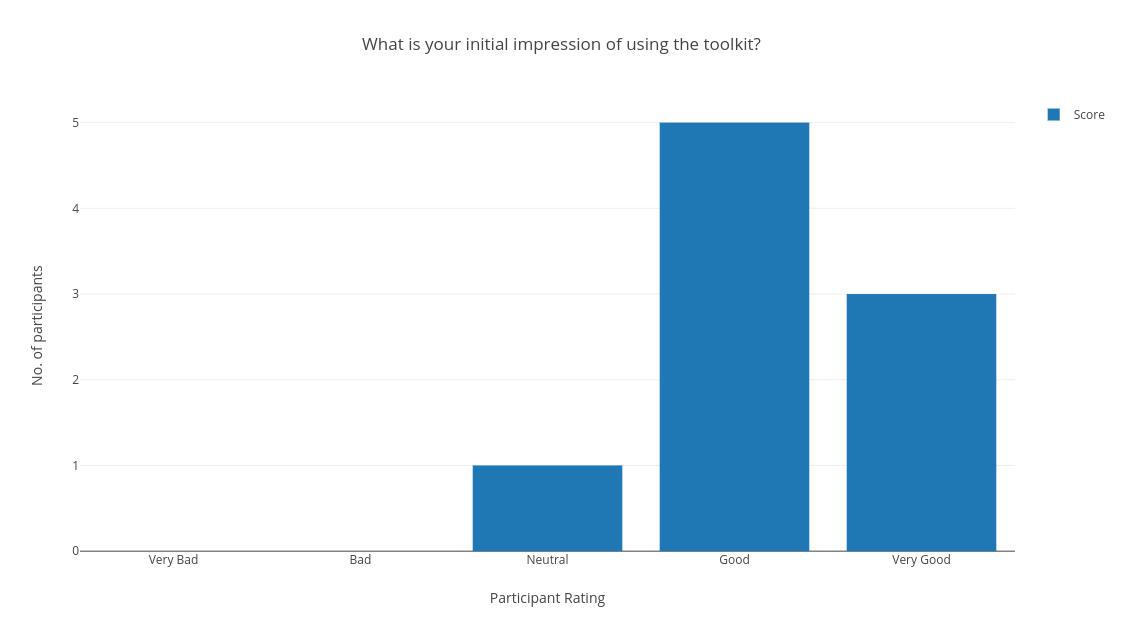
\includegraphics[width=\linewidth]{dissertation/eval_1_q3.png}
\caption{Q3}
\end{subfigure}
\hfill
\begin{subfigure}[h]{0.45\linewidth}
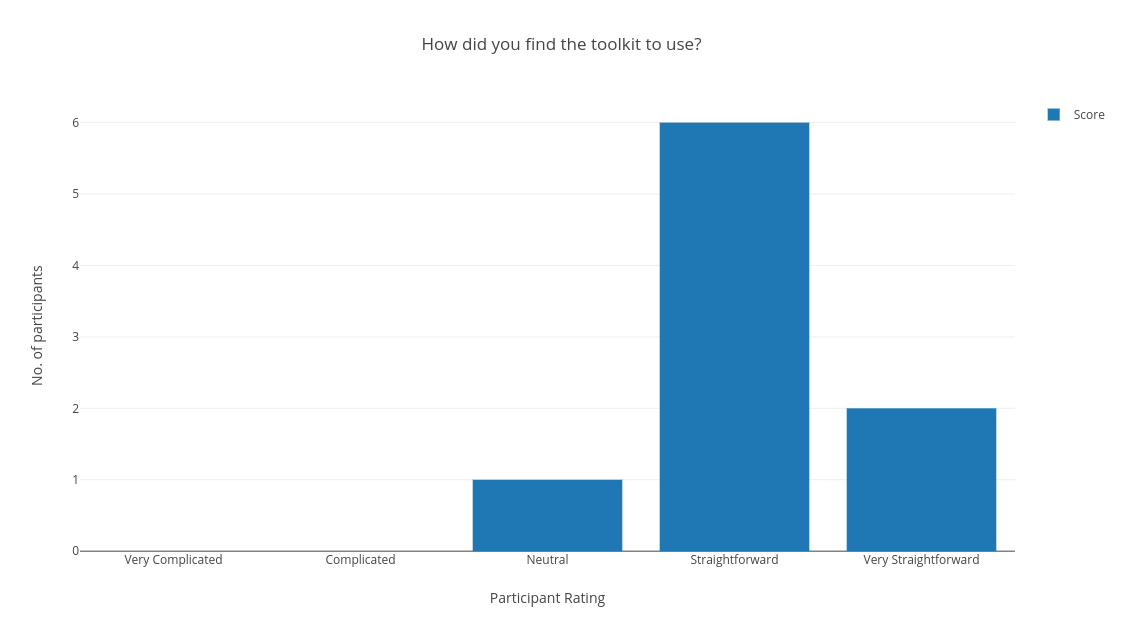
\includegraphics[width=\linewidth]{dissertation/eval_1_q4.png}
\caption{Q4}
\end{subfigure}
\hfill
\begin{subfigure}[h]{0.45\linewidth}
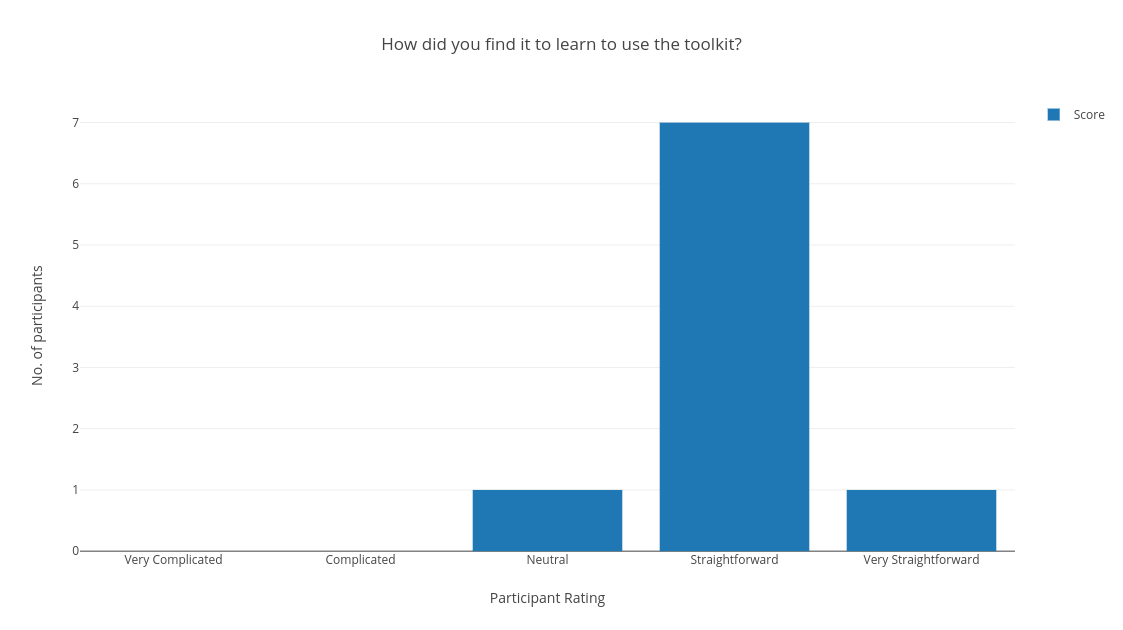
\includegraphics[width=\linewidth]{dissertation/eval_1_q5.png}
\caption{Q5}
\end{subfigure}
\hfill
\caption{Quantitative results from the questionnaire}
\end{figure}

The above three figures best represent the usability of the system as found by the participants of the application. In all three cases the majority of participants found that the initial impression of the toolkit was good and that the participants found it straightforward to both use and learn. Upon examining the data in context we see that the participants with a lot of technical background knowledge (i.e. extensive programming and Unity knowledge) were the participants who viewed the toolkit as being very straightforward to use with one also saying it was straightforward to learn. This is as expected though it is unknown if such users would soon encounter limitations within the toolkit and desire additional functionality not provided by it. It is likely that such users might consider switching to alternative toolkits rather than develop the functionality themselves from scratch. The SVRA toolkit however was not developed with such users as a priority, rather it was concerned with the non-technical users as a priority. Considering their views on the toolkit, we see that all viewed the toolkit as being straightforward to use and learn and rated their initial impression of it as being either very good or good.

\subsection{Qualitative Results}
\label{sec:evlauationqual1}
In addition to the quantitative questions, two open questions were included in the questionnaire. The first was to ask the participants to provide feedback on aspects of the system they found particularly confusing or difficult to use, whereas the second asked the participants if there was any additional features they would like to see included in the toolkit. The responses to this and any additional qualitative feedback were then analysed using the open, axial and selective coding method \cite{openaxebook} with the feedback summarised as follows:

\subsection{Usability Issues}
Concerning the usability of the system the key topics discussed were as follows:

\textbf{Cohesion:} For developers unfamiliar with VR development using Unity and the SteamVR SDK, the function of the SVRA toolkit in the development process can be confusing. Two participants did comment on this during the interviews where they highlighted they did not fully understand how the SVRA toolkit worked with the SteamVR SDK and how both worked with Unity. A third participant initially attempted to use both the toolkit and the SteamVR SDK simultaneously which will not work for toolkit specific operations. That is they attempted to use the SVRA scripts for making objects grabbable with the SteamVR SDK ``default Player prefab'' which setups up the camera and controllers under the SteamVR SDK system. Attempting to mix both systems will simply result in errors and as they are not compatible in such a way. Although for experienced developers this is not an issue, for new developers attempting VR development for the first time this can be confusing and a source of errors during development. A document explaining the roles of the SteamVR SDK and SVRA toolkit and how they are both used by Unity could be produced to assist first time developers in their understanding.
 
\textbf{Controller Configuration:} Two critiques of the controller configuration system employed by the toolkit were suggested during the first evaluation. The first was to switch the setup logic from the action-button to button-action system. As a round of A/B testing was intended to address this directly, this feedback validated the need to perform this during the next evaluation. A second comment made by several participants concerned the default button configuration for the controllers. The default configuration of the controllers for this evaluation was for the grip button to pickup objects and the trigger button to interact with objects. However, participants for who this was their first opportunity to use the Vive headset found the grip buttons on the Vive controllers to be difficult to press and felt that the trigger was a more intuitive button to press for object pickup. 

\textbf{Learning the Event Bridge:} Several participants stated that the event bridge was initially difficult to understand although once they had worked through several examples scenes that it became easier to understand and use. Although it was expected that this was the most difficult component of the toolkit and a tutorial for using it was produced prior to the evaluation, participants who attempted to learn it through experimentation struggled more with the component. One suggestion made was to make a video equivalent of the tutorial, a suggestion that is discussed in Section \ref{sec:conclusionfuturework}.

\textbf{Script Naming:} An issue with the script names which was observed during the evaluation and later confirmed by several participants during individual interviews was that scripts used internally by the toolkit behind he scenes were often being confused with the scripts used to setup interactions using the toolkit. This caused confusion as participants mistakenly attached internal scripts to objects rather than their intended script. As the toolkit did not notify the participants that the attached scripts were for internal use and should not be attached to objects the participants mistakes went unnoticed. Although the supplied documentation did make mention of the difference between included scripts some participants chose to ignore it in favour of a more hands on method of learning the toolkit through experimentation. This is one behaviour of the participant which was overlooked during the development of the toolkit and so measures should be taken to account for such users by for example hiding the internal scripts from the user. 

\textbf{Unity Integration:} One observation that was made during the evaluation was that the experienced Unity developers had a much easier time learning the toolkit as should was expected. The comments from experienced Unity developers regarding the toolkit were that it was straightforward to use, integrated as they expected and would fit into their existing Unity work flow. For the toolkit to be a success it must comply with the expectations of experienced Unity developers which it has as was demonstrated by the praise during the evaluation. 

\subsection{Additional Features}
Participants were also asked for suggestions of features they would like to see implemented in the toolkit with the following being suggested:

\textbf{Additional Player Actions:} One participant requested that additional actions be integrated into the toolkit such as the ability for users to inventory items or movement system such as teleportation. The desire for a teleporation system to be include was echoed by another participant in particular whose envisioned application could not be created due to the lack of locomotion system included in the toolkit. This is discussed in particular in Section \ref{sec:conclusionfuturework} though a teleportation system would be the next large feature to be incorporated into the toolkit and would have had time permitted during the development cycle.  

\textbf{Audio Functionality:} One participant with a particular interest in audio wished to see some form of audio functionality added to the toolkit and not overlooked and excluded from inclusion. They believed that some novel forms of audio interactions in addition to the more traditional would be a beneficial feature included in the toolkit. 
\textbf{Additional Sample Scripts:} Several requests for one off example scripts where suggested for implementation into the toolkit. One was a script to attach to the floor of the platform the player was walking on to detect if they had walked off the edge. Similarly this could be setup to not allow the player to walk through a wall or object within the world as well. Other suggestions included the ability to control the camera and world using the controllers or allowing for a scene to be reset to its original state via a button input. 

\textbf{Custom Editor Windows:} One participant with extensive Unity believed that custom editor windows would further enhance the usability of the system for non-technical users. This as previously discussed in Section \ref{sec:designnoeditorwindows} while beneficial for non-technical users was determined to be unnecessary due to the time constraints enforced on the project. It remains however one method by which the project could be improved as discussed in Section \ref{sec:conclusionfuturework}.

\textbf{Example \& Tutorials:} Suggestions were made for various different tutorials to be created to assist with the learning to use the toolkit. Some of the suggested tutorials were oriented more as towards first time VR developers and should include topics such as the SteamVR SDK which are already available on the web. A related suggestion was for the inclusion of more example scenes as the majority of participants found experimentation with these to be an excellent method of learning to use the toolkit. A suggestion was made for these to be more game-like in design to highlight the potential of the toolkit further. 

\subsection{Discussion}
\label{subsec:evlauationdiscuss1}
None of the participants had any prior VR development experience and had a mixed technical background with some having a lot of technical knowledge whereas others had none at all. While this shows positive results in that 8 out of 9 participants were able to implement their intended application and stated they would use the toolkit again it does come with one limitation. Due to the lack of prior experience with other toolkits a direct comparison cannot be made between the toolkit and an existing system. While this does limit the extent of the conclusions which can be drawn from the evaluation, as discussed in Section \ref{sec:evaluationlimitation}, the received response is viewed as evidence of a success. With the exception of one participant whose envisioned application required teleportation, a feature not included in the toolkit, all of the participants were able to create their, albeit simplest, applications within the fixed time limit opposed on the event. The majority of participants found the toolkit to leave a good initial impression and found it straightforward to learn and use with one quoted as saying \textit{``I didn’t think it would be that easy''}. 

The system is not without its flaws though with several key areas for improvement being highlighted during the interviews. The participant response in this regarded depending both on their background technical experience and envisioned use of the toolkit. Participants with prior technical experience typically suggested the addition of new features and functionality, in contrast to the participants with less of a technical background who suggested the system be improved through the addition of more tutorials and example scenes. They also desired some explanatory document that outlined who the SVRA toolkit, SteamVR SDK and Unity all worked together. As it was intended for a short development period to occur between the first and second evaluations it was important to strike the correct balance of new feature development and usability and training improvements. A detailed account of the changes made is found in Section \ref{subsec:evlauationchanges1}.

The evaluation method itself is not without its flaws and these too are worth discussing. Firstly as none of the participants had prior experience developing VR applications a direct comparison between the SVRA toolkit and existing toolkits could not be made. Given the nature of the project, a university dissertation project, finding multiple participants with extensive background experience to make a direct comparison would prove difficult, hence why the decision was made for the third round of evaluation be conducted as an expert interview with an experienced technical developer (Section \ref{sec:evaluationround3}). A second limitation of the evaluation was the time constraint enforced on the event which once training time was accounted for did not allow the participants to experience the full breadth of features included in the toolkit. The majority of participants instead opted to use a reduced subset of the toolkit's functionality. This reduced subset did included all of the key components included in the toolkit: controller configuration, grabbable objects, interactive objects and triggering some function using the event bridge, hence although the entirety of the toolkit was not tested by every participant the main components of the system were tested. This is a more realistic usage of the toolkit as one expects that the majority of users would only require a subset of functionality to create their application and avoid the irrelevant functionality entirely as was observed to occur here.

\subsection{Changes in response to first round}
\label{subsec:evlauationchanges1}
After the first round of evaluation was performed the feedback received was analysed for improvements to be made to the system prior to the second round of evaluation occurring. The key changes to the toolkit prior to the second round of evaluation occurring are summarised below:

\textbf{Additional Training Scenes:} The first round of evaluation showed firsthand that example scenes were very beneficial to assisting new developers learn to use the toolkit. This was especially proven to be true in the second round of evaluation (Section \ref{sec:evaluationround2}) but a set of 3 additional training scenes were produced prior to the second round of evaluation in response to the user feedback from the first round of evaluation.

\textbf{Audio Functionality:} As discussed in the first round evaluation discussion (Section \ref{subsec:evlauationdiscuss1}) one of the participants when asked for future functionality suggestions felt that some form of sound event examples would be beneficial. As a sound framework was aimed for in the requirements as highlighted in Section \ref{sec:requirementsfunctionalnonfunctional} it was decided to implement and audio triggering system into the toolkit, whereby users could specify audio to trigger using the event system and to easily customise the audio file being played. 

\textbf{Controller Configuration Button-to-Action Logic:} Due to time constraints both versions of the controller configuration system were not implemented prior to the first round of evaluation occurring. Instead only the action-to-button approach, as seen in toolkits such as VRTK, was implemented. The reverse logic approach was designed and implemented prior to second round of evaluation and A/B testing performed on the two methods to verify the believe that this would be the preferred approach by users. 

\textbf{Hiding Internally Used Scripts:} One of the key observations made during the first round of evaluation was that some users had trouble distinguishing between the internally used scripts and the scripts used within the toolkit to perform actions. One of the most common ways of adding a script onto an item in Unity is through the Inspector window for an object, where users can search for part of the script’s name and have a list of possible scripts to attach to the object produced. In order to reduce this confusion it was setup so that any script used internally by the toolkit was hidden in this view. 

\section{Evaluation Round 2: Individual Interviews}
\label{sec:evaluationround2}
Following the first round of evaluation a second, more individual focused, round of evaluation was conducted. Although the aims were similar to the first, the more individual focused nature of the evaluation method was believed to be able to provide a more in depth insight into any shortcomings of the usability of the toolkit to implement some function. The method, discussed in full below, had participants be given an overview of the toolkit and then tasked them with setting up three example scenes to achieve some functionality and afterwards a semi-structured interview was held using a variant of the questionnaire used in the first round of evaluation. The questionnaire is included in Appendix \ref{sec:appendeval2questions}. Similar to the first round of evaluation the results and feedback were collected and the toolkit went through another round of changes as is discussed below, with a complete set of the results gathered included in Appendix \ref{sec:appendeval2results}.

\subsection{Method}
\label{sec:evlauationmethod2}
The evaluation method employed in the second round of evaluation was designed to be more individual driven than the first evaluation. While the first provided a broad evaluation of the entire system due to the nature of the evaluation method it was difficult to monitor a participant execute common tasks. Doing so would prove useful as it would uncover any problematic areas of the design in which users where either confused or the system could be streamlined. A total of 8 participants were interviewed in the second round of evaluation. None of the participants had previously used the toolkit prior to the evaluation taking place, that is none were included in the 9 participants of the first round of evaluation. The method used during the second round of evaluation was as follows. First participants were given an overview of the toolkit, its purpose and the general process by which to create applications. They were then presented, alongside the documentation for the system, two tasks in the form of Unity scenes. For both tasks the associated Unity scene had already been created and participants were required to merely setup the required SVRA scripts in order to make the scene operational. 

The first task required the participants to setup the controllers for use and two objects within the scene. The first object simply required the user add the grabbable object script onto the object and the second required adding the same script but applying a modification onto it. Participants were given the freedom to either add the suggested modification of making the object snap to some custom orientation or some other modification of their choosing. The second task required that participants use some of the more advanced aspects of the toolkit. Specifically it required that the participant setup the controllers and then establish an event bridge between an button which was required to be made interactive and a sphere object. Participants were required to alter the colour of the sphere upon interacting with the button. The second task required users setup two grabbable objects and establish an event bridge between them so that upon grabbing one of the objects an event such as a color change or grabbable toggle.

It was decided to perform a round of A/B testing in the second round of evaluation to determine the preferred user controller configuration approach, as was discussed in Section \ref{sec:decisioncontrollersetup}. Due to the small number of participants it was believed that rather than split the participants and give half of participants the action-button logic and half the button-action logic that all participants would be given both systems and asked to justify their preference. This would be achieved due to the two task nature of the evaluation, where half of the participants would be required to use the action-button logic on the first task and the button-action logic on the second task and where half of the participants would be required to use the button-action logic on the first task and the action-button logic on the second task. The feedback received from this is discussed in Section \ref{sec:evaluationround2ab}. 

\subsection{Quantitative Results}
\label{sec:evlauationquant2}

\begin{figure}[h]
\begin{subfigure}[h]{0.45\linewidth}
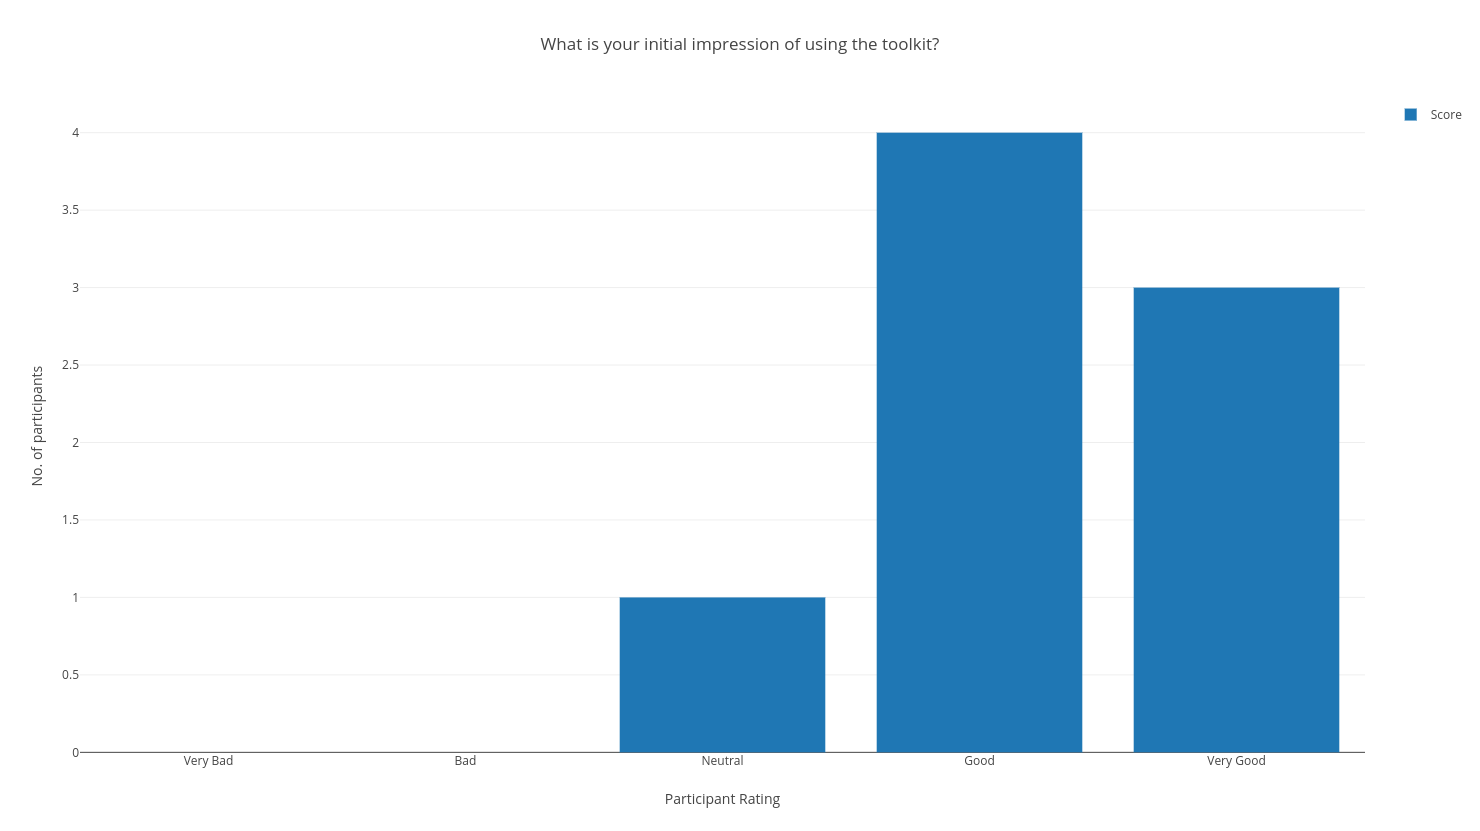
\includegraphics[width=\linewidth]{dissertation/eval_2_q3.png}
\caption{Q3}
\end{subfigure}
\hfill
\begin{subfigure}[h]{0.45\linewidth}
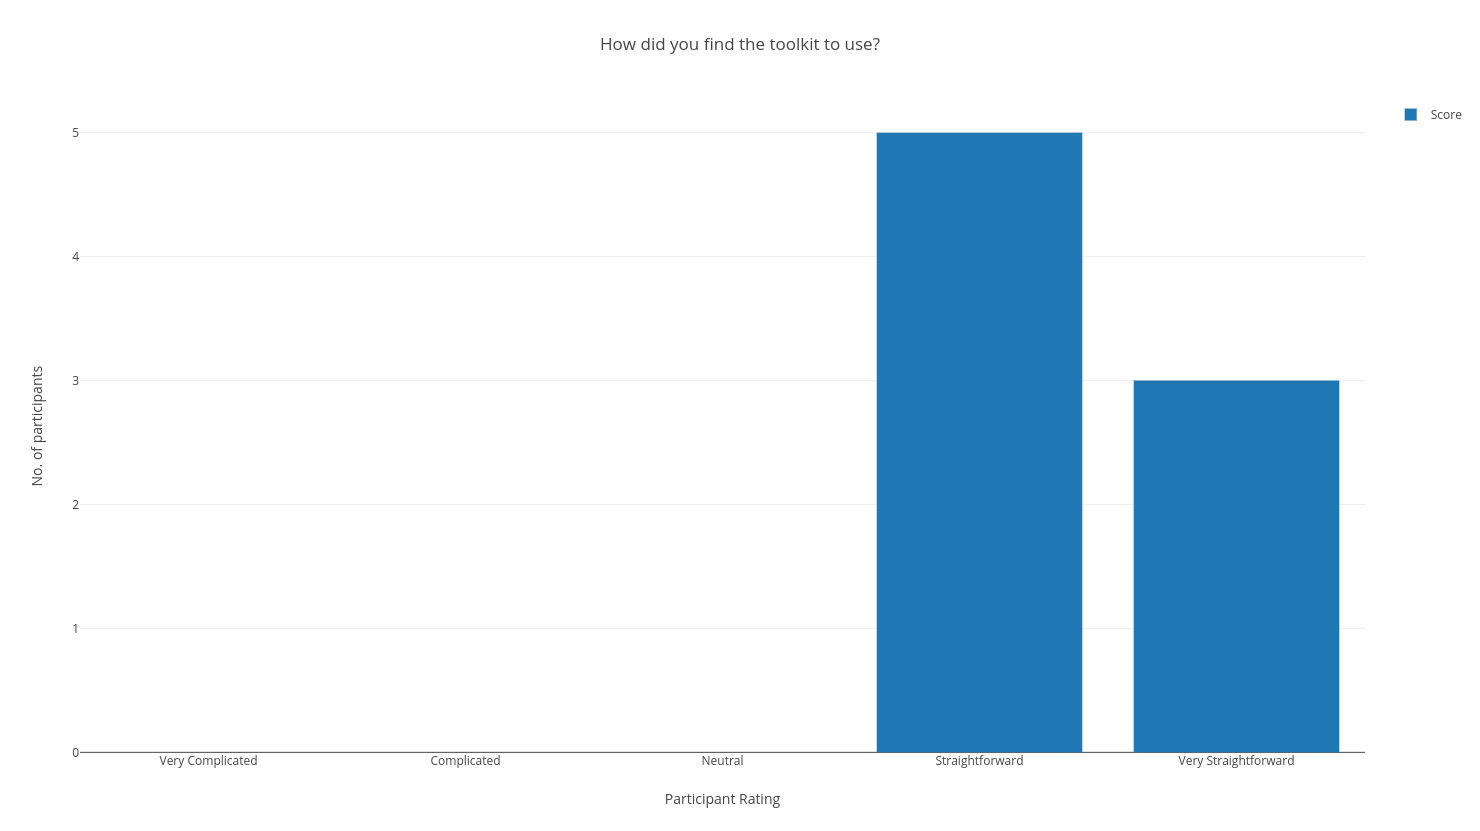
\includegraphics[width=\linewidth]{dissertation/eval_2_q4.png}
\caption{Q4}
\end{subfigure}
\hfill
\begin{subfigure}[h]{0.45\linewidth}
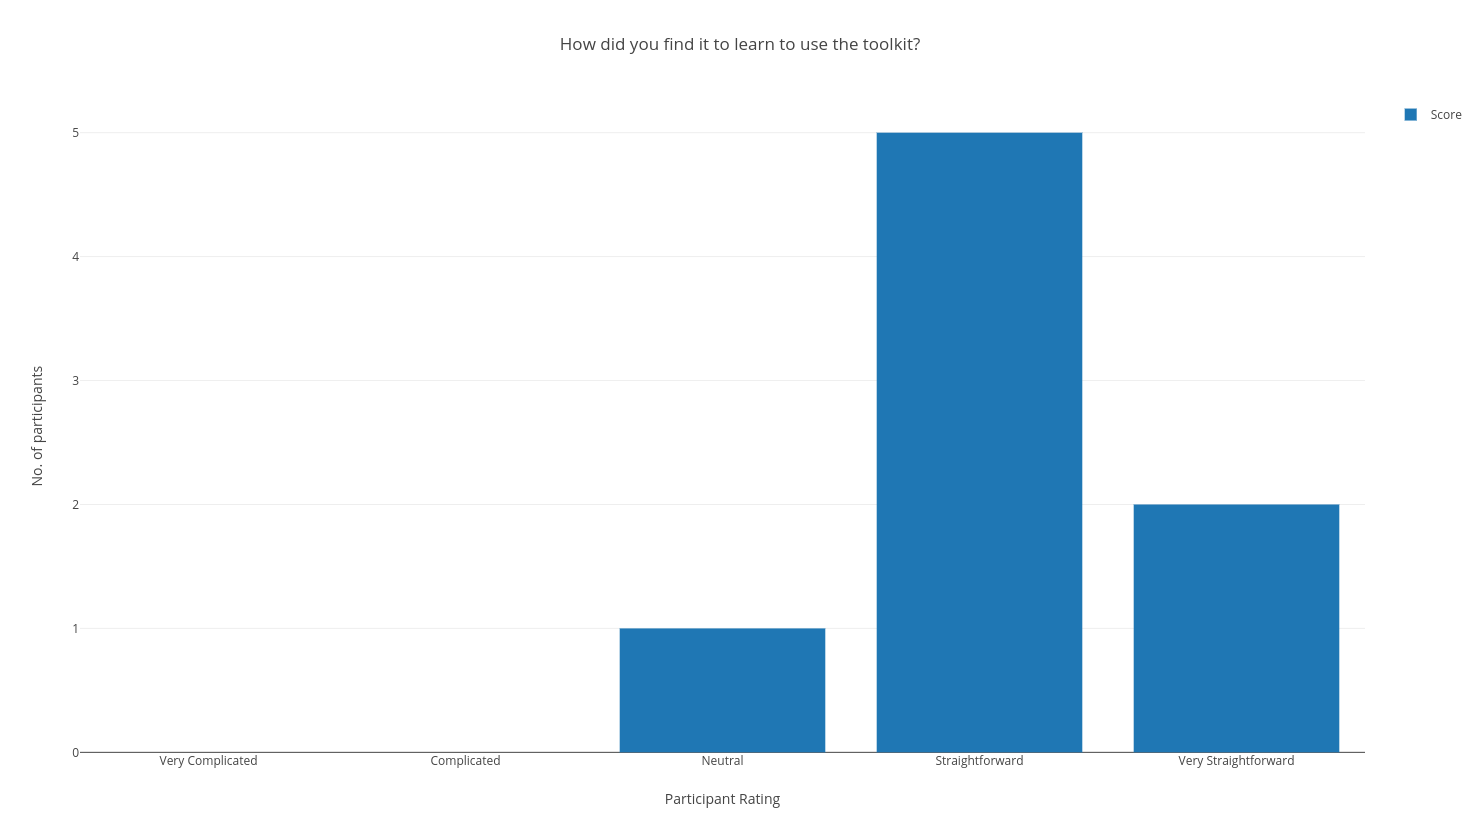
\includegraphics[width=\linewidth]{dissertation/eval_2_q5.png}
\caption{Q5}
\end{subfigure}
\hfill
\caption{Quantitative results from the questionnaire}
\end{figure}

The questions asked during the first round of evaluation concerning the usability of the system were also asked of participants in the second round of evaluation, with the above graphs showing the participant responses. Although the second evaluation used 8 participants opposed to the 9 used in the first we can see that some marginal improvements are seen in regards to how the participants found learning and using the system. The results, as a whole, once again are positive and further confirm the desire for a simple to use VR development toolkit on the market. 

\subsection{Qualitative Results}
\label{sec:evlauationqual2}
As with the first round of evaluation, the feedback recieved from the second was collected and analysed using the open, axial and selective coding method. The feedback is summarised as follows:

\textbf{Confusing With Naming Conventions:} One topic that was highlighted previously in the first evaluation and again in the second was the naming conventions used within the toolkit. Some participants felt that the names of scripts did not best represent the script's purpose. For example the script name of ``SVRA\_ColorToggle'' should be changed as its functionality had changed to change between a user defined range of colours opposed to toggling between two colours. Additionally it was noted that some of the participants were required to check the functionality of scripts in the documentation as the name did not fully suggest the script's purpose and use. Also noted was the familiarity between the naming conventions used by the SteamVR SDK and the SVRA toolkit as one participant mistakenly added a SteamVR script to the object believing it to be the SVRA equivalent. Finally one non-technical user commented that the naming system contained a lot of ``technical'' and ``Unity specific'' terminology and that for them this was not helpful, \textit{``The term prefab is meaningless to someone like me who isn't familiar with all of the Unity terminology''}.

\textbf{Single Point of Setup:} One participant, with a significant amount of prior Unity development experience, stated that they expected there to be some functionality to create a ``manager-like object''. This object would be one onto which multiple scripts would be attached and the objects within the scene then told to inherit all of the behaviours of this ``manager object''. This idea of a single point of setup is interesting and would have some benefits for non-technical users and is further discussed in Section \ref{sec:conclusionfuturework}.

\textbf{Training Tutorial Set:} The desire for a structured set of tutorials was highlighted once again during the second round of evaluations. Although more example scenes were provided to participants to assist them to learn to use the toolkit several participants believed that a more structured approach was needed. The suggestion was to create a structured set of tutorials which would start with the most basic functionality of the toolkit and progressively introduce and teach users how to use the more complex functionality of the toolkit. This approach was later adopted as discussed in Section \ref{sec:implementationchangesduetoeval2}. Another suggestion made was to produce a set of video tutorials alongside the written tutorials. This is discussed further in Section \ref{sec:conclusionfuturework}.

\subsection{A/B Testing Results}
\label{sec:evaluationround2ab}
As previously stated a round of A/B testing was conducted in order to select the logic of the controller configuration of the toolkit. The method, as described above, saw all participants use both systems and then asked to select and justify their preference. The results found are that 6 of the 8 participants favoured the button-action logic and 2 of the 8 favoured the action-button logic. This shows that the hypothesis suggested in \ref{sec:decisioncontrollersetup} was correct as the participants felt that selecting the action to map to each button of the controller was the more intuitive system. One participant gave the example of setting up the custom shortcuts or buttons on a mouse or video game controller, \textit{``when I think about configuring a peripheral such as shortcut buttons on a mouse or the buttons of a video game controller I expect to select the button and then assign the shortcut onto it''}. Aside from the intuitiveness of the system, participants with a technical background also believed that the reverse logic, of mapping buttons onto a list of actions, would scale poorly as new actions and functionality were added to the toolkit over time.

\subsection{Discussion}
\label{sec:evlauationdiscuss2}
Although further suggestions for improvements was suggested during the second round of evaluation, with some of the changes implemented in response outlined below, the system once again proved itself as an easy to learn and use toolkit. One of the key aims of the toolkit was to make a drag and drop VR development toolkit. Attainment of this goal was captured during this round of evaluation as one participant commented \textit{``It's just like Alice\footnote{Alice is an educational, drag-and-drop programming language for teaching computer programming} for Unity and VR development''} environment for learning computer programming.] Similar to the first round of evaluation, the second round of evaluation also suffered from the limitation of the participants not having any prior development experience making VR applications. The positive feedback received does however further indicate the desire and need for a simple VR development toolkit on the market.

\subsection{Changes in response to second round}
\label{sec:implementationchangesduetoeval2}
In addition to providing an insight into user's preference of controller configuration system (Section \ref{sec:evaluationround2ab}) the second round of evaluation also highlighted several ways in which the system could be improved before its public release. The following changes were implemented as a result of the received feedback:

\textbf{Controller Configuration System Decision:} With the A/B testing performed during the second round of the evaluation (Section \ref{sec:evaluationround2ab}) showing that the vast majority of users preferred the logic of mapping the actions onto the buttons of the controller it was selected as the implemented system for controller configuration within the toolkit. Additionally it was at this point that the aforementioned virtual buttons in Section \ref{sec:decisioncontrollersetup} were implemented into the toolkit as their omission was necessary for a fair comparison between the two proposed systems during the A/B testing. 

\textbf{Renaming Class Names:} One subtle but significant change suggested during the second round of evaluation was to alter the names of a lot of the scripts which a user uses whilst using the toolkit. The feeling was that some were either ``too technical'' or did not best represent the functionality of the script. This was primarily concerned with the sample scripts where a name such as SVRA\_ColorToggle was renamed SVRA\_ChangeColor and SVRA\_MaterialToggle was renamed to SVRA\_ChangeMaterial. Similarly the controller configuration prefab was renamed from ControllerManagerPrefab to ControllerSetup.

\textbf{Extensive Documentation \& Examples:} As stated previously, the second round of evaluation (\ref{sec:evaluationround2}) showed the need for extensive documentation to be produced for the toolkit. This not only includes additional example scenes and written API-like documentation for the toolkit but also included tutorials for how to use the toolkit. As a result of this the documentation was refined and expanded to better explain each of the scripts provided by the toolkit. More example scenes were created each of which highlighted a different feature of the toolkit were produced. Finally alongside a set of written tutorials several training examples were developed. These were scenes with the objects pre-setup and were designed to be used with the written tutorials to guide users through setting up objects and interactions using the toolkit. A complete set of the written tutorial sheets is included in Appendix \ref{sec:appendtutorialsheets}.

\section{Evaluation Round 3: Expert Interview}
\label{sec:evaluationround3}
The final evaluation conducted was an expert interview with an experienced VR developer who has experience primarily with VRTK but also other VR development toolkits as well. This was hoped to provide some insight into how the toolkit compared against other existing toolkits. The methodology used differed from the first and second evaluations rounds as the expert was instead given an overview and walk through of the toolkit which was followed by a discussion. As with the first and second rounds of evaluation, the method of open, axial and selective coding \cite{openaxebook} was used to analyse the feedback received from this interview. A transcript document is available in Appendix \ref{sec:appendevalexperttranscript} but a summary of the key identified categories is as follows:

\textbf{Controller Configuration:} While the controller configuration system was found to be straightforward by the expert one comment they did have regarded setting the controllers up to perform different functions. That is if the two controllers are setup to have different functionality is there a way of saying that the one controller will always be the right controller and the other always the left controller. This is a concern as SteamVR in the past has changed where for a period it was the case that the first controller turned on was always the right controller. This was later changed so that one of the controllers would always be the right controller. Forcing one controller to be the right and another during the left might reduce the risk of errors due to such underlying technology changes breaking existing functionality in the future. 

\textbf{Custom Editor Windows:} The application of custom editor windows for the project, as previously discussed in Section \ref{sec:designnoeditorwindows}, was discussed. Specifically while the benefits of custom editor windows were mentioned the implementation of them was deemed unnecessary unless it was essential for a custom window to be implemented, \textit{``it’s rarely worth it unless it’s something you really, really need to have a nice layout for with a nice explanation''}. This was due, as was previously mentioned, to the difficult nature of their development and the large amount of development time typically needed for their implementation, \textit{``They're a pain''}, and should only be implemented after the development of the feature has finished, \textit{``do it at the very end when [the feature] it is locked down''}. 

\textbf{Event Bridge:} The event bridge system was discussed at length, especially in comparison to the VRTK event system. Where the VRTK approach includes the event system into every interactive item, the SVRA approach abstracts the event system out into a separate component. While simpler to use for first time developers the expert felt that \textit{``perhaps a more advanced event bridge is needed''}. This would either be an extension to the existing event bridge system or a separate more advanced event bridge. The idea being that the simple event bridge would be offer the basic functionality provided by the current system and the more advanced would provide a more technical and capable system. The advance system would handle the concerns of the expert of the existing system such as \textit{``What if I wanted to define a series of steps to occur all of the objects on a grab event?''}, \textit{``Can I stop some event midway through execution?''} and \textit{``Can I pass some argument to the event bridge?''}. This is an excellent opportunity for future work on the system and is discussed in full in Section \ref{sec:conclusionfuturework}.

\textbf{Evaluation Flaw \& Extension To Existing Toolkit:} When discussing the previous rounds of evaluation conducted on the product the expert highlighted one flaw in the evaluation method used on the product, the lack of direct comparison with an existing toolkit. This evaluation flaw is discussed in full in Section \ref{sec:evaluationlimitation}, though the primary reason for its omission was the time required from the evaluation to be performed not being feasible due to the context of the product's development. As discussed with the expert, the current evaluation shows that there exists the desire for a simplified VR development toolkit but whether this should be an entirely new toolkit or a custom interface for an existing toolkit remains unknown. Development of such a custom interface to simplify VRTK was discussed at length during this evaluation with the proposition for the work included in Section \ref{sec:conclusionproofofconcept}.

\textbf{Object-Controller Connections:} A comparison between the SVRA and VRTK methods of establishing the connection between objects and the controller was also made. The SVRA method, as outlined in Section \ref{sec:decisionobjectinteractiondesign}, includes the logic of how to attach the object to the controller directly into the grabbable object script. The VRTK method abstracts away the attachment logic to create a more flexible system for technical developers. As the expert commented \textit{``What happens when I want a different type of attachment altogether?''}. Under the current implementation this will require a significant amount of technical knowledge of the developer as the system was designed to be all encompassing for a non-technical developer. One remedy to this might be to alter to create a more advanced method of attachment system whereby developers can write their own attachment script logic and then select it from a drop down list of attachment scripts, similar to how the highlighting system is implemented by the toolkit, as discussed in Section \ref{sec:decisionhighlightingsystem}. 

\textbf{Suggested Features \& Improvements:} During the interview the expert also suggested some usability improvements and potential features for the toolkit. A minor usability change that would greatly improve a non-technical users experience concerns the situation where one script relies on another to function correctly. If a script attached onto an object requires another script in order to function correctly then if the required script is not already attached then automatically attach it onto the object when the other script is attached. This is a very logical idea and from a user's perspective very helpful as it ensures errors do not occur due to the omission of some necessary script. Aside from the extensions outlined earlier, such as the extensions to the event bridge and controller configuration systems, the expert also suggested a bridging system be created between existing toolkits. Such a system would allow the user to create a simple prototype application using the SVRA toolkit and when a more advanced toolkit was necessary then switch to the toolkit while maintaining the established logic setup in the prototype. Such a system would effectively be required to translate one toolkit's logic into anothers and would likely prove to be a significant technical challenge. 

\section{Evaluation Limitation}
\label{sec:evaluationlimitation}
One limitation of the evaluation process performed during this project which must be addressed is the lack of direct comparison of the SVRA toolkit against an alternative such as VRTK. Where the results of the evaluation conducted prove the desire of an easy-to-use VR development toolkit exists whether this should be an entirely new toolkit remains to be seen. Rather than build an entirely new toolkit, the approach could be taken to simplify an existing toolkit as is discussed in Section \ref{sec:conclusionproofofconcept}. An evaluation directly comparing the two systems would have provided some insight into this topic. This form of direct comparison evaluation was not performed primarily due to time constraints of the project's completion and the time investment that would be required of the participants to perform the evaluation. Due to nature of the project, a university dissertation project, the majority of participants were students with no previous VR development experience. For a fair, direct comparison to be made between the SVRA toolkit and another toolkit (VRTK) participants would be require training to reach the same level of competency with the two toolkits, after which they would be asked perform a series of tasks within both toolkits. Afterwards they would be interviewed to discuss their experience of using both toolkits. This would require a significant time investment of the participant and so it was deemed that for such a round of evaluation it would be unfeasible to perform the evaluation a significant number of participants for a definite conclusion to be drawn.

\section{Evaluation Conclusion}
\label{sec:evaluationconclusion}
The SVRA toolkit sought to create an easy to use development toolkit aimed at non-technical developers for creating VR applications. The evaluation conducted on the toolkit shows that the desire for a simple to use VR development toolkit exists on the market. Feedback was positive throughout the three rounds of evaluation conducted with the vast majority of participants rating the system as being ``good'' or ``very good'' and stating they would reuse it again for future VR development. The evaluation methods used were limited however by the lack of direct comparison against an existing toolkit as discussed previously. While we can conclude that the desire for such a system is clear whether the SVRA toolkit performs better than an existing toolkit cannot definitively be said. It is suggested from the collected results that it would due to the high scores by which participants rated it as being straightforward to both use and learn how to use. Such praise further validates the claim that the created system meets the initially proposed requirements. 

The implementation of the system compared against the originally proposed MoSCoW requirements must also be discussed. While not all of the initially proposed functional requirements of the system (Section \ref{sec:requirementsfunctional} were met the system does fulfill all of the non-functional requirements (Section \ref{sec:requirementsnonfunctional} set of it. Concerning the unfulfilled functional requirements of the system some such as the ability to easily change controller models of the controllers were discovered to be supported by the SteamVR SDK natively and did not break compatibility with the SVRA toolkit when implemented into the application. Others such as a locomotion or automated testing system are good points of future feature development as discussed in Section \ref{sec:conclusionextendingtoolkit}. Feature discovery did play a role during the development where features such as the virtual buttons for the touchpad where thought of and implemented during the development stage of the project. As previously stated all of the non-functional requirements of the project have been met however. The SVRA toolkit provides a code free VR development experience where users are able to easily modify objects and interactions with a minimal number of clicks. With the exception of the aforementioned flaw in the event bridge system it does provide minimal user repetition though as stated this could be further improved as suggested in the potential areas of future work in Section \ref{sec:conclusionextendingtoolkit}. The toolkit itself can be very easily customised with the addition of new features of modification to existing ones by a technical developer. Despite not all of the original functional requirements of the system being met, the positive reception seen in the various stages of evaluation, the attainment of the non-functional requirements and a road map provided for implementation of the remaining functional requirements in the suggestions for future development it is believed that the SVRA toolkit successfully meets the goals originally set out for it. 

\chapter{Conclusion}
This chapter presents directions for the future development and direction of the toolkit. The toolkit may either be viewed as a standalone product for future development and suggestions are included for what such work might be or alternatively the product could be viewed as a proof-of-concept for work to done on an existing system. The report concludes with a summary of the project and its accomplishments.

\section{Future Work}
\label{sec:conclusionfuturework}
The SVRA toolkit provides two directions for future development. Either the system is viewed as an entirely new toolkit which can be further developed as an open source project or it can be viewed as the proof-of-concept system to justify the work needed to build a set of simplified custom interfaces for an existing toolkit. Both of these directions for the future work of the project are discussed below.

\subsection{Proof-of-Concept System}
\label{sec:conclusionproofofconcept}
The evaluation of the SVRA toolkit proved there is a user demand for a simple to use VR development toolkit but as discussed in Section \ref{sec:evaluationlimitation} due to a limitation of the evaluation it cannot be definitely said whether this should be a new toolkit, such as the SVRA toolkit, or an extension to an existing toolkit that simplifies using it. The suggestion to extend an existing toolkit was made during the expert interview (Section \ref{sec:evaluationround3}) where what such an extension to an existing toolkit might be was discussed. Viewing the product as a proof-of-concept for work to be done an existing toolkit, the first piece of future work would be to create a set of prototype, simplified custom interfaces for an existing toolkit. Due to its popularity it is likely that this would be VRTK. The created interfaces would provide the user with three levels of complexity ``Simple'', ``Medium'' and ``Advanced''. This would be used to filter the amount of displayed options on the interface thereby reducing the complexity of using the toolkit by streamlining the UI. This approach would reduce the need to redevelop much of the work already implemented by an existing toolkit such as VRTK. It would also immediately have access to a much larger pool of potential users due to the existing users of the existing toolkit. Extending an existing toolkit also brings the benefit of not requiring existing users to learn a new toolkit and is usable by developers currently in development of applications built using the existing toolkit who are unlikely to switch toolkits mid-development.  

This approach however does not removed some of the other problems found in existing development tools such as those as highlighted by the clients in Section \ref{sec:requirementsdndmeeting}. Problems such as the ``Configuration Chains'' which occur during the setup of more complex interactions or the need to add multiple scripts onto objects where a single setup script should suffice would remain in the toolkit if this approach for future work was taken. Furthermore reliance on an existing toolkit brings the add risk as was discussed in Section \ref{sec:decisionnewtoolkit} where one of the main reasons for developing a new toolkit was to allow for complete creative control over the project. Reliance on other toolkits brings creates the risk of the reliant toolkit's development halting and this risk was highlighted firsthand during the development of this project as the sole, lead developer of the VRTK project announced in January 2018 that his involvement with the project was over. Currently the project's future development as an open source project remains to be seen but as of March 2018 it looks unlikely that the development community surrounding the toolkit will step up and continue its development. This belief based on comments made by the lead developer of the VRTK project who justified his exit by claiming that it was in part due to the lack of assistance being provided by the community in development of the toolkit. Therefore it is my opinion that a new toolkit, such as the SVRA toolkit, is instead what is needed rather than an extension to an existing toolkit to reduce the complexity assoicated with using it. 

\subsection{Extending The Toolkit}
\label{sec:conclusionextendingtoolkit}
Rather than build an extension to an existing toolkit, work could instead be done to extend the functionality of the SVRA toolkit. Primarily this takes the form of either new functionality to be added to the system or extensions being made to existing features within the system. Some suggestions for both approaches are presented below as a means of improving the existing system:

\subsubsection{Additional Functionality}
The following features are suggested as being beneficial additional functionality which could be added to the toolkit:

\textbf{Additional Hardware \& An SDK Management System:} Bringing the toolkit to additional hardware platforms was identified as something which would not be achieved during the development of this project (Section \ref{sec:requirementsfunctional}). Extending the toolkit to support additional hardware platforms remains a goal worth pursuing with the Oculus family of devices being the logical next hardware platform to target given their sizeable portion of the VR consumer market share. This would most likely require the introduction of an SDK management system into the toolkit which would serve as a single point of setup and be used to manage which SDK and hardware platform to build the application for.

\textbf{Automated Testing System:} 
A second feature originally proposed in Section \ref{sec:requirementsfunctionalnonfunctional} but one that did not see development was the proposed automated testing functionality. Nevertheless such a feature is worth pursuing. As discussed by the clients during the requirements elicitation meeting in Section \ref{sec:requirementsdndmeeting} the desire for a method of automating the testing process would save significant time during the development process. The following system is proposed as one potential solution. The feature might operate by the user being able to record their actions and then repeat them on demand during the testing process. This would allow the user to test functionality of the application by replaying the recorded set of actions and observing the results opposed to putting on the hardware and then testing the change to the application.

\textbf{Script Manager Object:} One suggestion made for an additional feature during the evaluation of the product (Section \ref{sec:evlauationqual2}) was for the inclusion of a ``manager-like object'' where a set of scripts could be added and objects told to inherit all of the scripts attached to this management object. Rather than set up every object's logic individually, this approach would only require users setup the object logic once on the manager and then point all the other objects at the manager to inherit it's behaviour. This is a interesting suggestion as it would streamline the development process and allows for a single point of modification should the behaviour of a set of objects with the same behaviour be required to be changed, opposed to  requiring the user change each object's logic individually as is currently the case.

\textbf{Teleportation System:} 
A final feature proposed in Section \ref{sec:requirementsfunctionalnonfunctional} but omitted due to time constraints is a movement, teleportation system. Teleportation is the most popular current form of movement found in VR applications and would be the next logical ``player action'' to be developed and included in the toolkit. With its inclusion this would give the SVRA toolkit a significant advantage over purely interaction based toolkits, such as the NetwonVR toolkit, which lack movement and teleportation functionality. 

\subsubsection{Extended Functionality}
The following are suggested improvements to existing functionality found within the toolkit which would improve the system:

\textbf{Advanced Event Bridge:} As discussed in Section \ref{sec:evaluationround3} the event system in the toolkit currently suffers from several limitations. Currently if the user wished to make say 20 objects alter colour upon interacting with a button this would require setting up the colour change script on each of 20 objects and then configuring the event bridge 20 times, once per object. To combat this problem an advanced variant of the event system is proposed for development. This advanced event bridge would allow multiple objects to be setup simultaneously to trigger the same way on some interaction event occurring. Using the aforementioned example again with this system, the color change upon the button being interacted with would change once and the list of 20 objects passed to it to all know to change color upon the interaction event being triggered. This would be a significant improvement regarding the usability of the event bridge system within the toolkit.

\textbf{Controller Improvements:} Several improvements could be made to the controller configuration system implemented by the SVRA toolkit. Firstly during the development of the project using swipe actions on the controller's touchpad as a form of input were prototyped. Such inputs would be configurable in the same way as the other buttons of the controller. For example the user would be able to map the grab action onto a down swipe of the touchpad. A second extension would be to include the omitted requirements for the controller configuration system as outlined in Section \ref{sec:requirementsfunctionalnonfunctional}. This would add an option to make the controller model invisible upon picking up an object, an effect frequently seen in within VR applications. Additionally it would add the ability to turn the controllers into physical objects to interact with objects within the application. A final extension is one that was suggested during the expert evaluation in Section \ref{sec:evaluationround3}. This would be to create a method by which you force one of the controllers to always be the left controller and the other controller to always be the right controller. This addresses the case where you have two controllers setup with different logic as the system might randomly assign one of the controllers to be the right and the other to be the left. Such a feature would ensure that the specified left controller receives the left controller logic indefinitely.

\textbf{Drawer Configuration System:} The proposed requirements for the project in Section \ref{sec:requirementsfunctionalnonfunctional} aimed to make the setup of common interactions within applications such as drawers and doors as straightforward as possible. The current implementation of this within the toolkit requires the user to configure the drawer using the Unity ``Configurable Joint'' object. This object is a much more flexible variant of the aforementioned Unity ``Joint'' object and for non-technical developers can provide challenging to work with. Instead a system could be created where the user provides the position of the start and end of the drawer's possible motion and then configure the joint automatically for the user. This would be a significant improvement for an inexperienced Unity user's use of the product. 

\textbf{Extended Scene Transition System:} An improvement which could be made to the scene transition system included in the toolkit would be to add the functionality for users to specify a custom loading scene area to use during the scene transition. This was a goal originally proposed in initial requirements of the system in Section \ref{sec:requirementsfunctionalnonfunctional} but one that was dropped during the development of the scene transition feature. Currently the feature allows for simple configuration of the transition zone by altering the attributes of the default provided area used to transition between scenes. The extension would allow the user to specify a custom Unity scene to use as the transition space. Allowing for custom loading spaces would dramatically increase a player's sense of immersion during scene transitions and as such is a beneficial feature to be included in the toolkit.

\textbf{Highlighting System Improvements:} The set highlighting effects within the toolkit currently only tints the colour or material of the object. An extension to this would be to increase the set of highlighting effects to include some more complex forms of highlighting. This could be effects such as the ability to outline an object or to allow the user to specify a colour or material to use as a highlighting effect. As discussed in Section \ref{sec:decisionhighlightingsystem} the VRTK highlighting system includes such options but requires users attach these to the object as individual scripts. The SVRA approach instead forces the developer to derive from the base highlighting script class and provides setup for the scripts via a drop down interface, thus providing the same functionality in a much more user friendly manner. 

\textbf{Physics System For Object Connection:} During the development of the system a more realistic physics system was prototyped, as discussed in Section \ref{sec:decisionobjectinteractiondesign}, for establishing the connection between the controller and the object being interaction with. Although this system was later dropped due to its additional complexity introducing bugs other aspects of the controller-object connection system, it collision system did appear slightly improved over the default system provided by Unity. Should these problems be fixed then its inclusion as an alternative controller-object connection would be an attractive addition to the toolkit. 

\textbf{Push Buttons:} Outlined in the requirements of the project in Section \ref{sec:requirementsfunctionalnonfunctional} was the desire for the creation of a class of buttons within the toolkit. The original vision for buttons was for the button to be triggered by being physically pushed with the controller opposed to the implemented solution of triggering the interaction by pressing a button on the controller. One obvious improvement then to the implemented button system would be include the originally envisioned button interaction method into the toolkit. By this method buttons would be triggered by being physically pushed by the user with the controller. A second improvement might be to build the event bridge system directly into the button class of objects as it is necessary to establish the button to trigger some event upon being pushed. This would improve the usability of the toolkit as it would not require the user to setup the object simply as a button rather than as a button and with the event bridge separately as is currently the case.

\textbf{Video Tutorials:} One idea which was suggested during the evaluation of the application would be to create a set of video tutorials for the application in Section \ref{sec:evaluationround2}. This was suggested first as a tutorial video for the event bridge component and again as a series of short videos which would guide users through the creation of increasingly complex examples. Given that VRTK produced similar videos explaining the example scenes included with the toolkit and that these videos proved a popular method of learning to use the toolkit, this idea is one worth pursuing to improve the documentation and learning resources available to users for the toolkit.

\section{Summary}
The objective of this project was to develop a VR toolkit aimed at non-technical users interested in the development of VR applications. Through speaking with experienced non-technical developers of VR applications (Sections \ref{sec:requirementsdrwilliamson} and \ref{sec:requirementsdndmeeting}) and by reviewing the existing popular toolkits on the market (Sections \ref{sec:contextnewton} and \ref{sec:contextvrtk}), the SVRA toolkit was designed to simplify the creation process involved in making VR applications. Despite not all of the originally proposed requirements (Section  \ref{sec:requirementsfunctionalnonfunctional}) being met, partially due to the effect of feature discovery providing some alternative functionality that was deemed more significant for the toolkit, the evaluation conducted on the system (Section \ref{sec:evaluationchapter}) suggests that the development was a success. Lacking from the evaluation was a direct comparison between the SVRA toolkit and existing toolkits and this would have proved very beneficial (Section \ref{sec:evaluationlimitation}) but its inclusion was unfortunately unfeasible due to the time constraints enforced on the project. The evaluation does show however that the desire and demand for an easy to use VR development toolkit exists and the SVRA toolkit in its current form is proposed as the first iteration of such a toolkit.

%%%%%%%%%%%%%%%%
%              %
%  APPENDICES  %
%              %
%%%%%%%%%%%%%%%%
\begin{appendices}

\chapter{Requirements Meeting Minutes Extract}
\label{sec:appendmreqmeetmins}
Included in the following pages are a PDF extract from the meeting minutes taken at the offset of the project. Within the extract are notes taken on the requirements and aims of the project as outlined by Dr. Williamson during our initial weekly meetings at the offset of the project. 

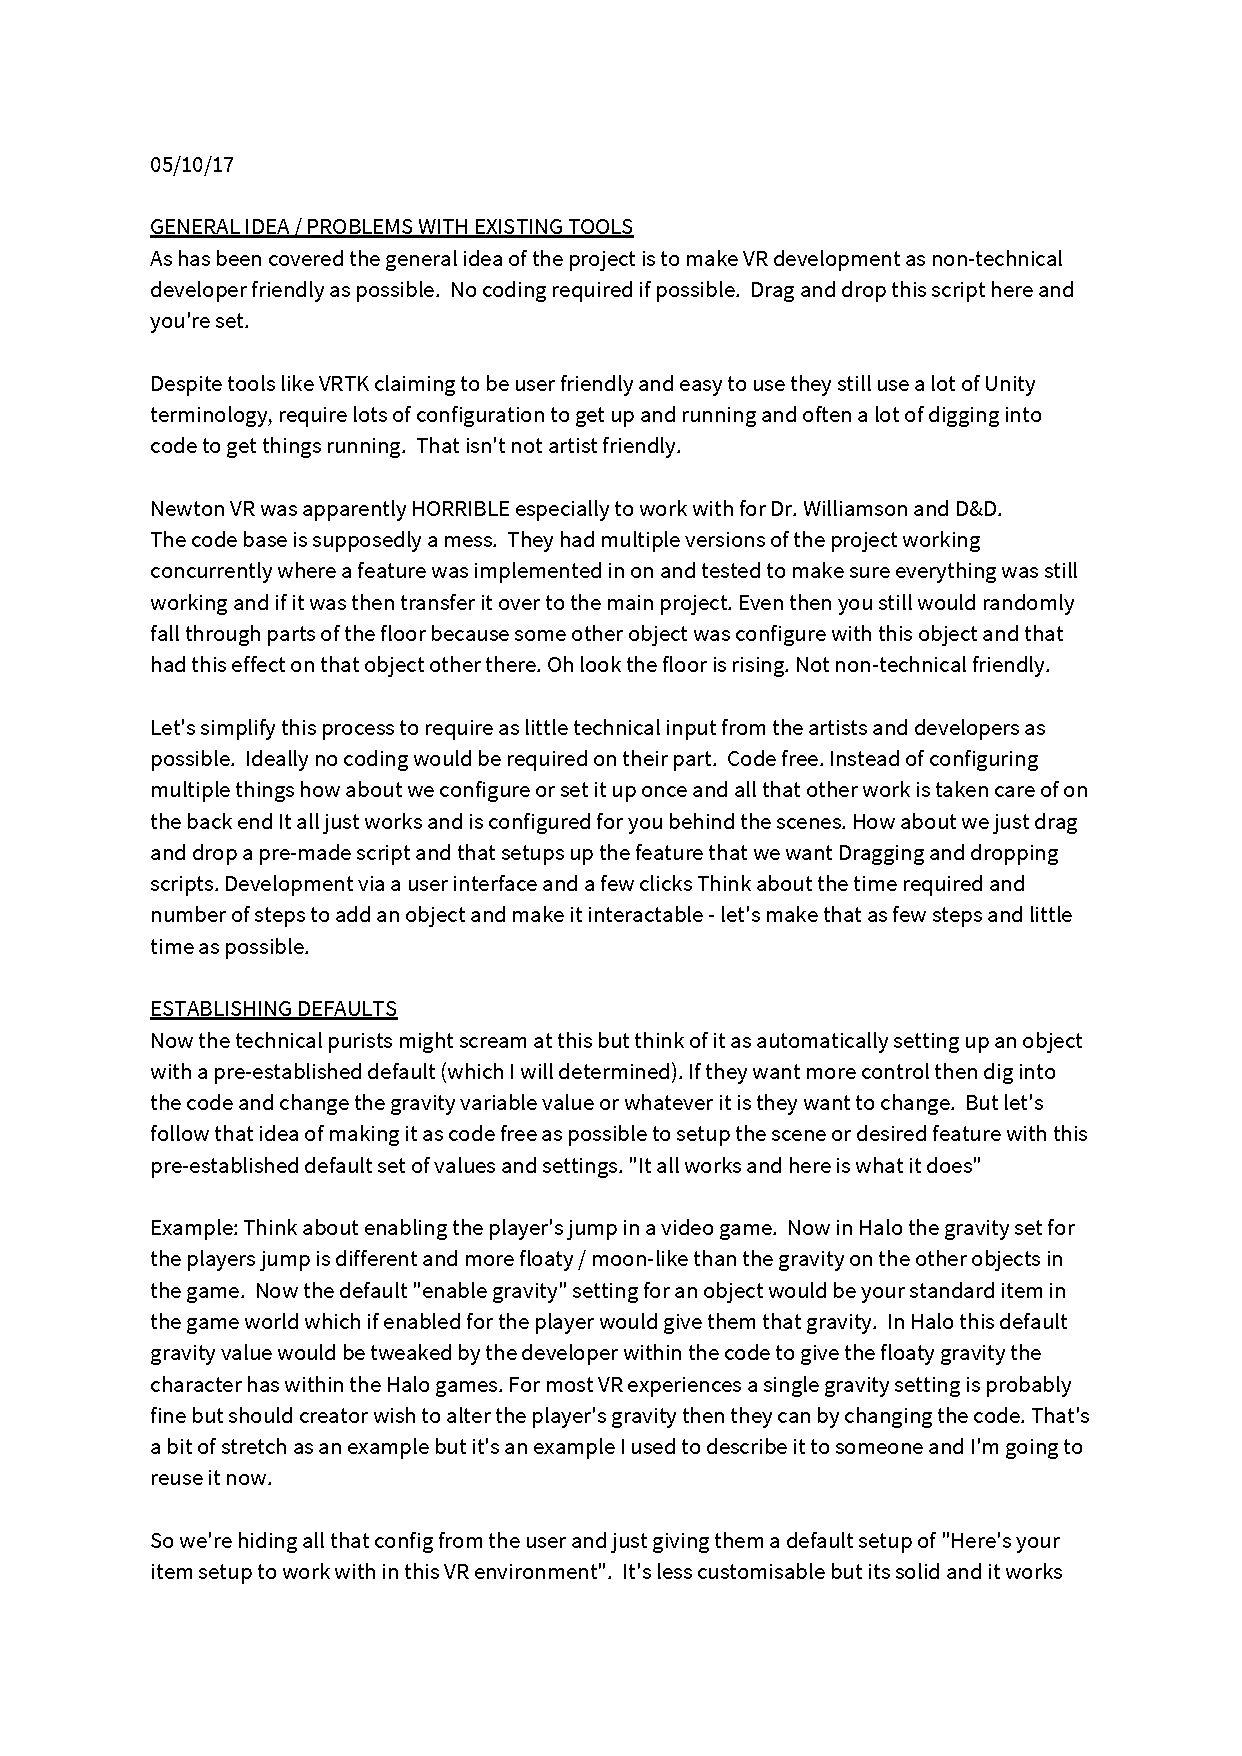
\includepdf[pages=-]{dissertation/pdfs/meetingmins.pdf}

\chapter{Client Interview Question Set}
\label{sec:appendclientinterviewquestions}
Included in the following pages is a PDF document which was produced as a set of questions and discussion points for the client meeting held with artists from Dennis and Debbie club.

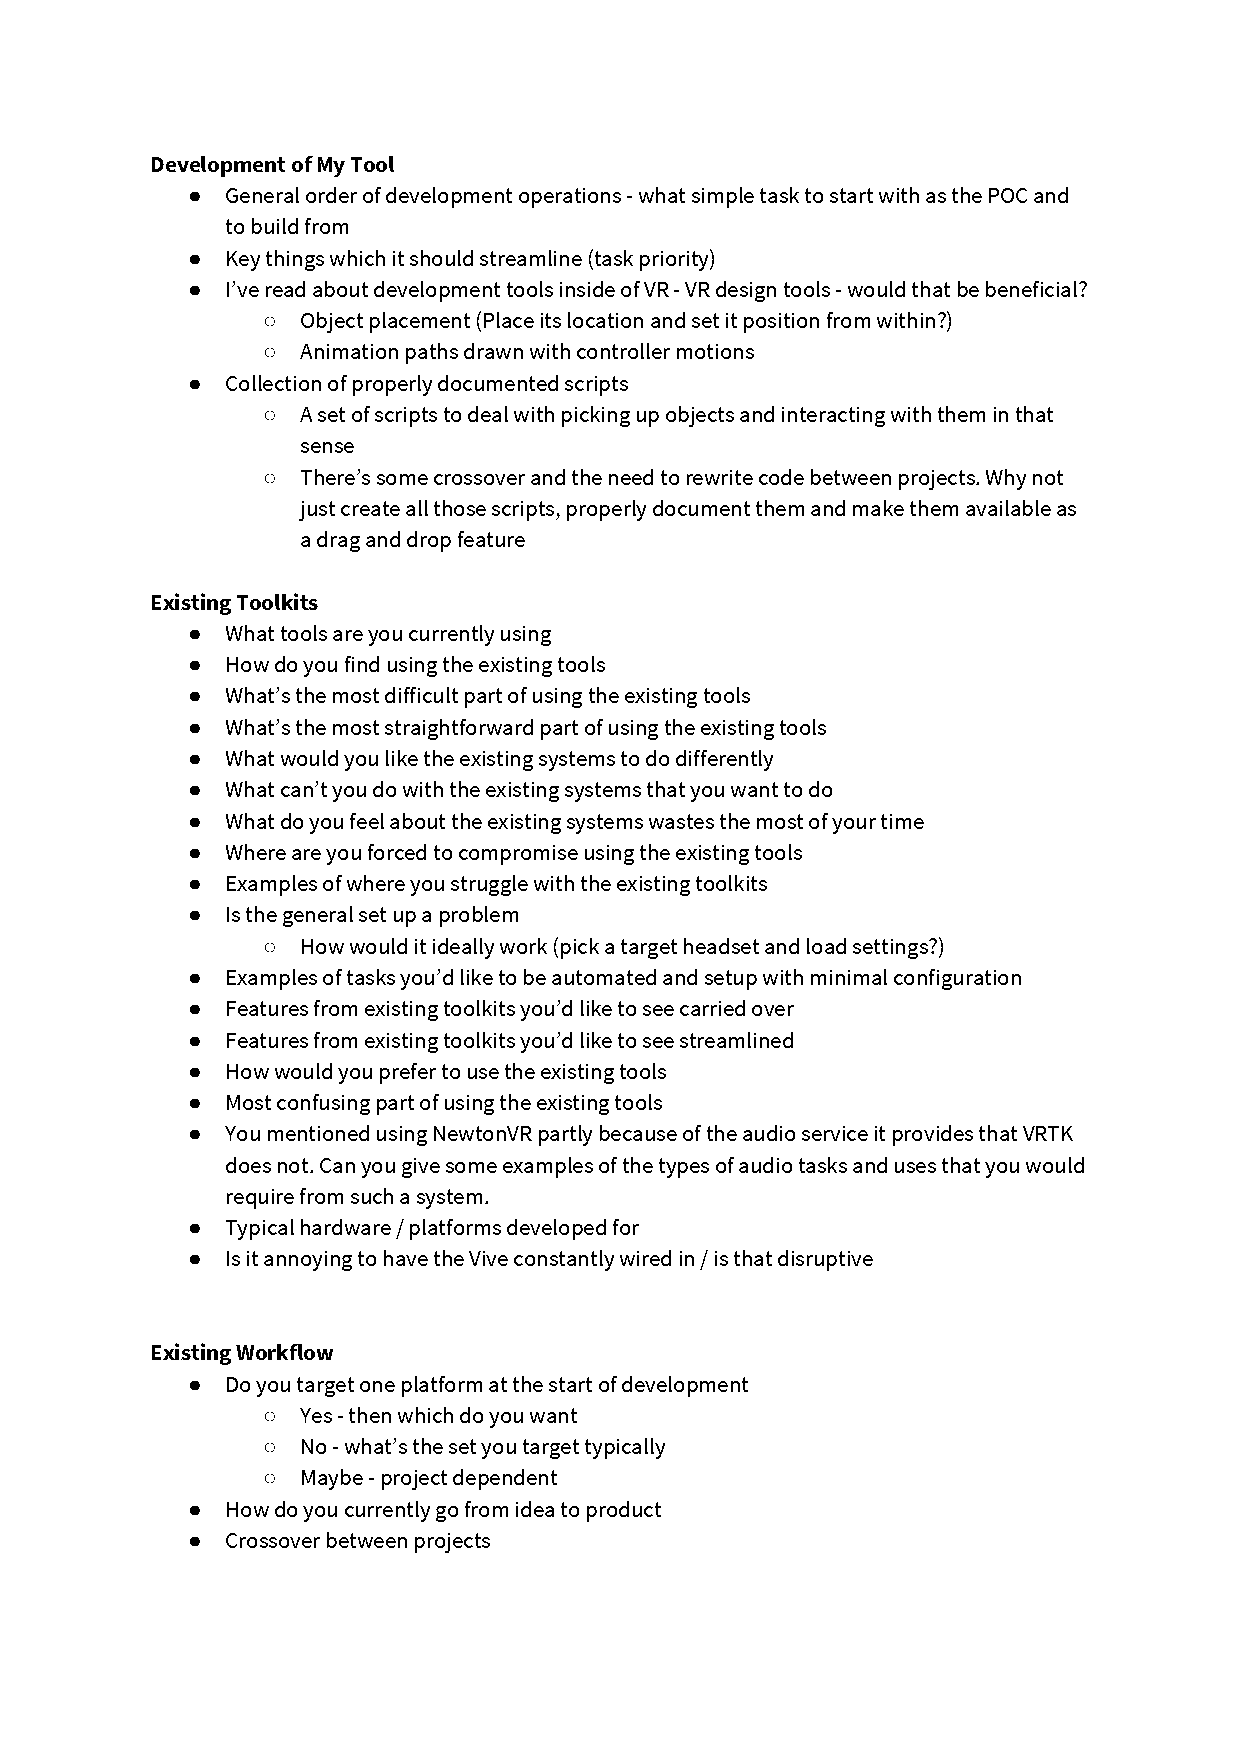
\includepdf[pages=-]{dissertation/pdfs/requirements_questions.pdf}

\chapter{Client Meeting Transcript}
\label{sec:appenddndtranscript}
Included in the following pages is a transcript document which was produced as a result of the meeting with artists from Dennis and Debbie club. It contains a summary of the discussion that was had as well as some additional information added in post to contextualise what is being discussed. Included is the PDF document that was produced.

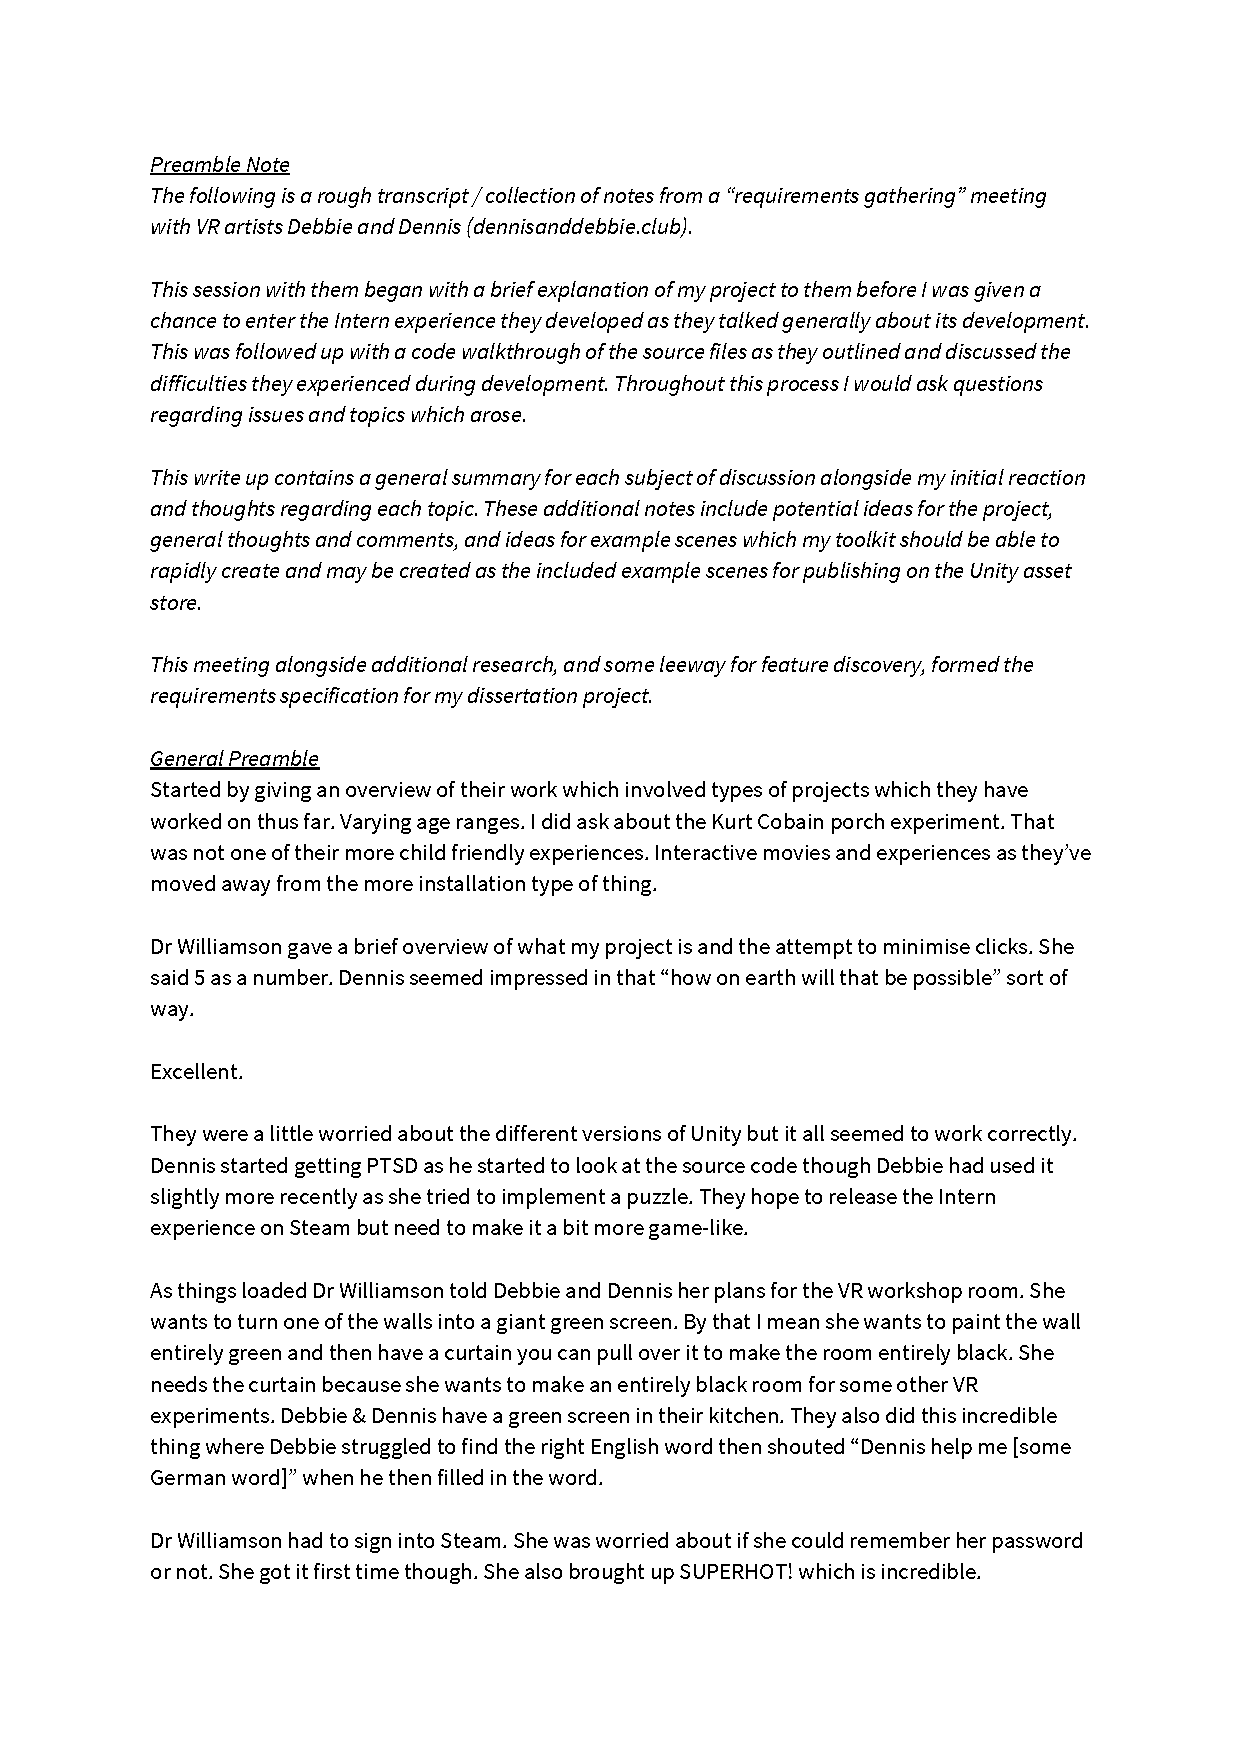
\includepdf[pages=-]{dissertation/pdfs/dndtranscript.pdf}

\chapter{Requirements Categories}
\label{sec:appendreqcat}
Included in the following pages is a PDF document which was produced during the analysis of the requirements for the project. This performed to categorise the different types of requirements suggested during the various requirements meetings held for the project and to assist with the translation into a set of functional and non-functional requirements for the project. 

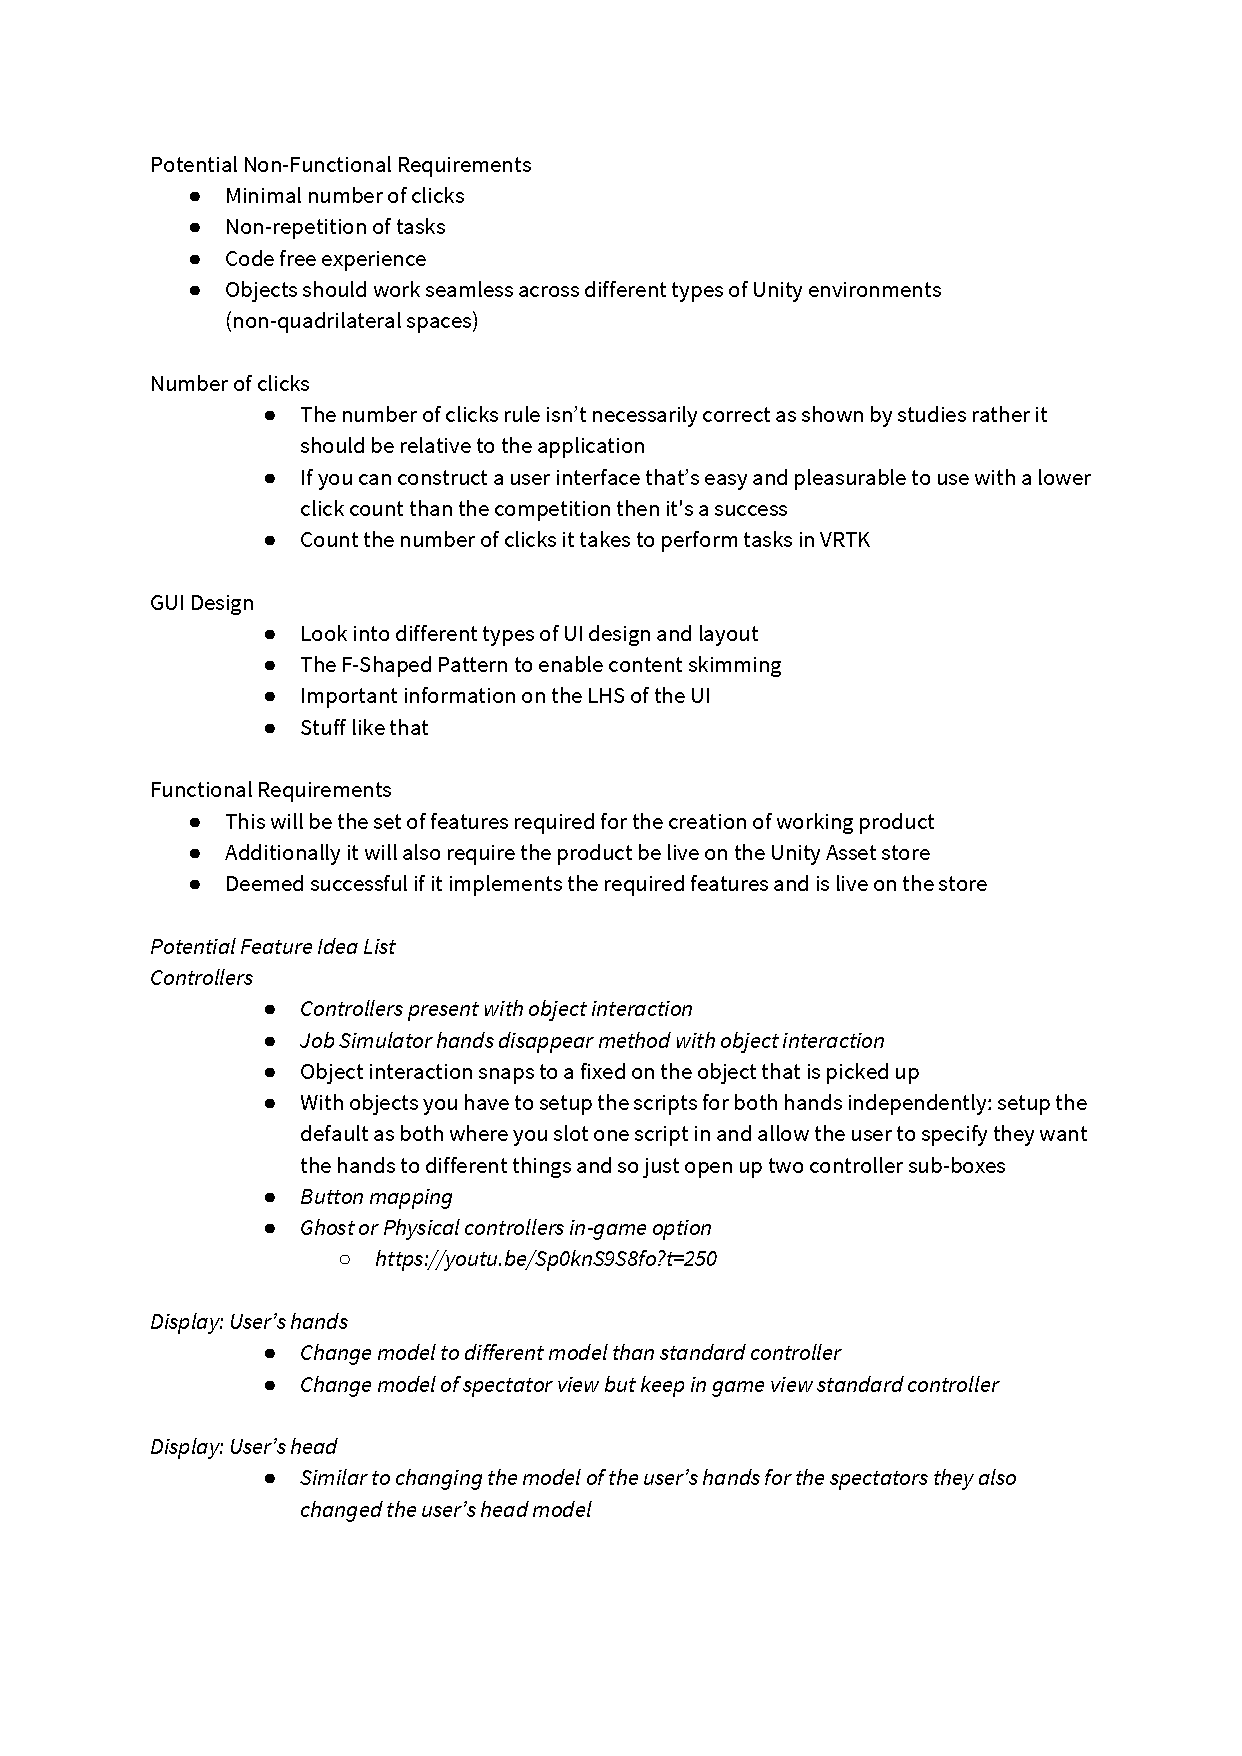
\includepdf[pages=-]{dissertation/pdfs/requirementscats.pdf}

\chapter{MoSCoW Requirements Lists}
\label{sec:appendmoscow}
Included in the following pages is a PDF document which was produced to represent the entire set of features considered for inclusion in the toolkit. 

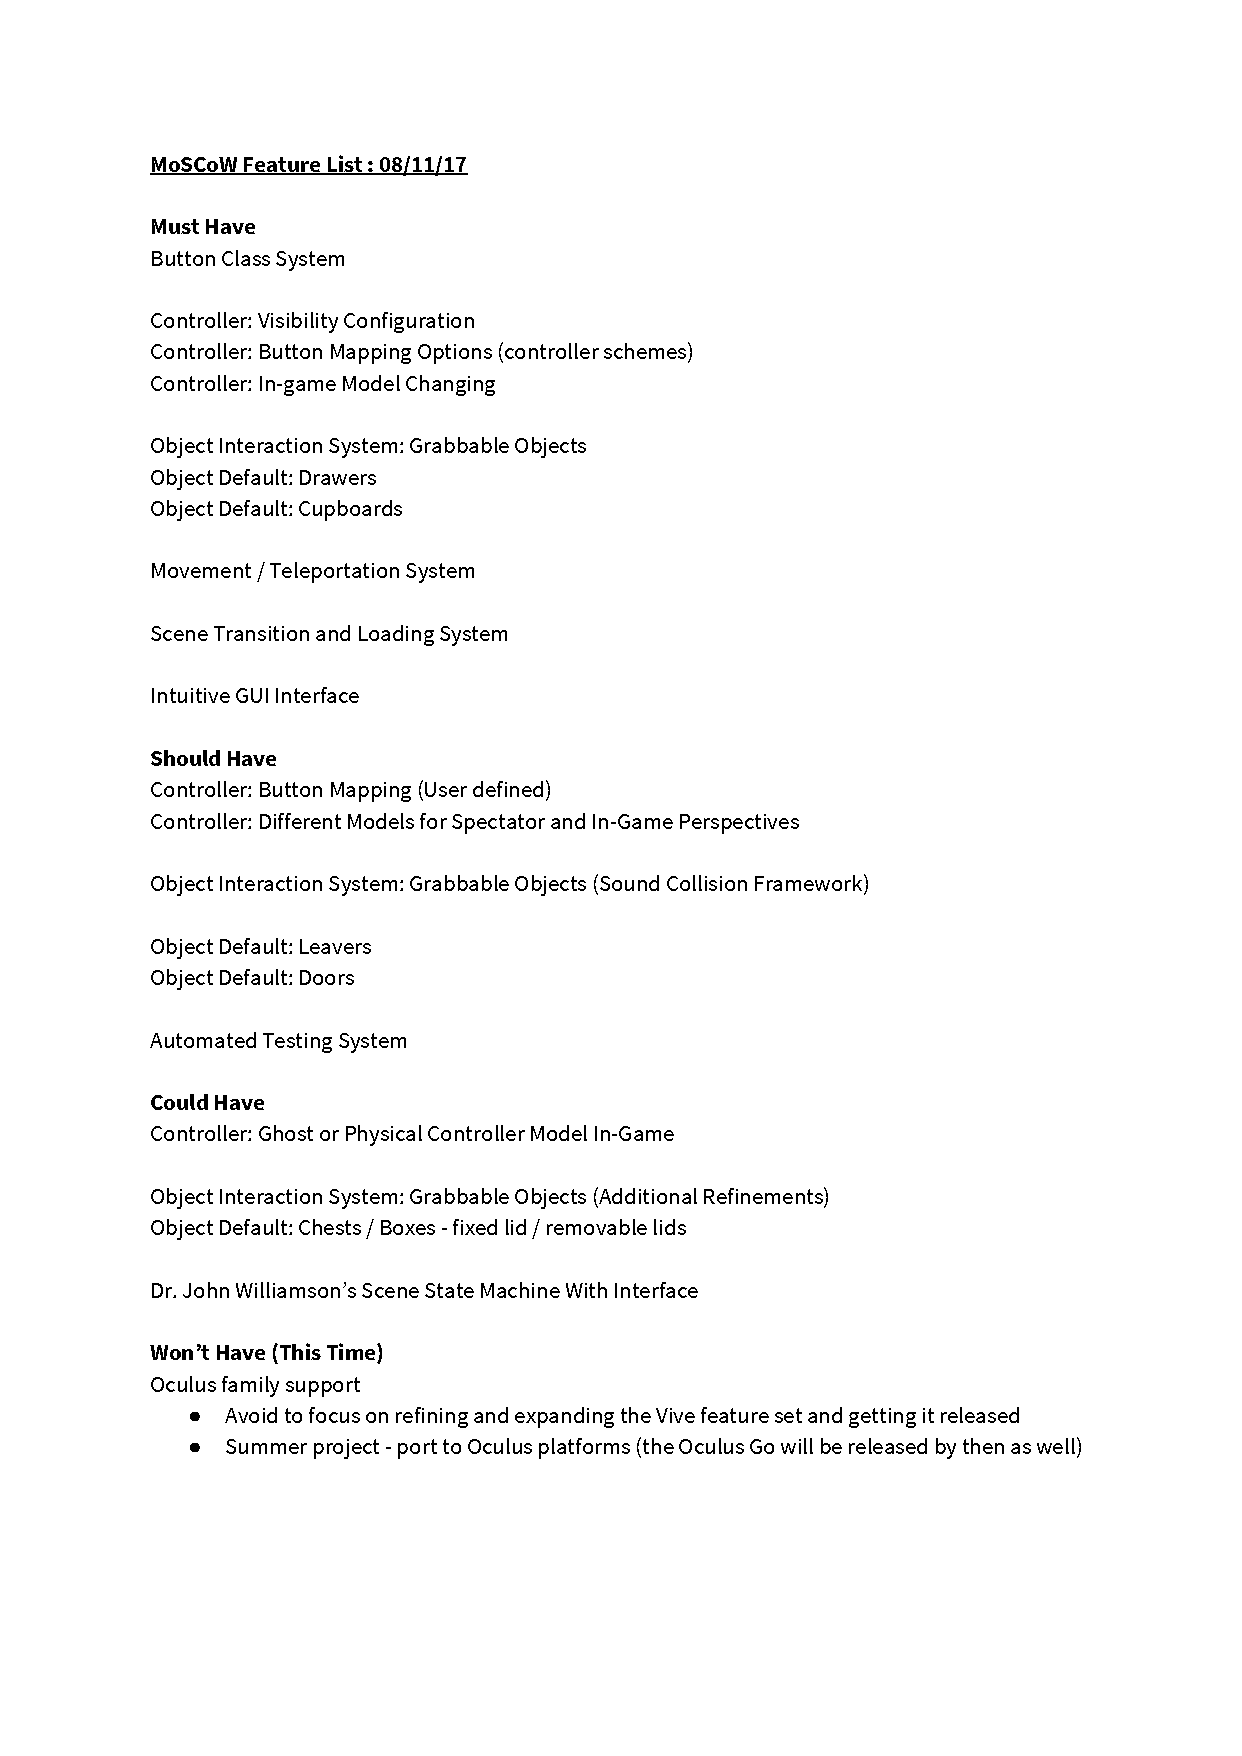
\includepdf[pages=-]{dissertation/pdfs/moscow2.pdf}

\chapter{Toolkit Documentation}
\label{sec:appendscriptdocs}
Included in the following pages is a PDF document which was created to provide users with an overview of the features included in the toolkit and how to use it. 

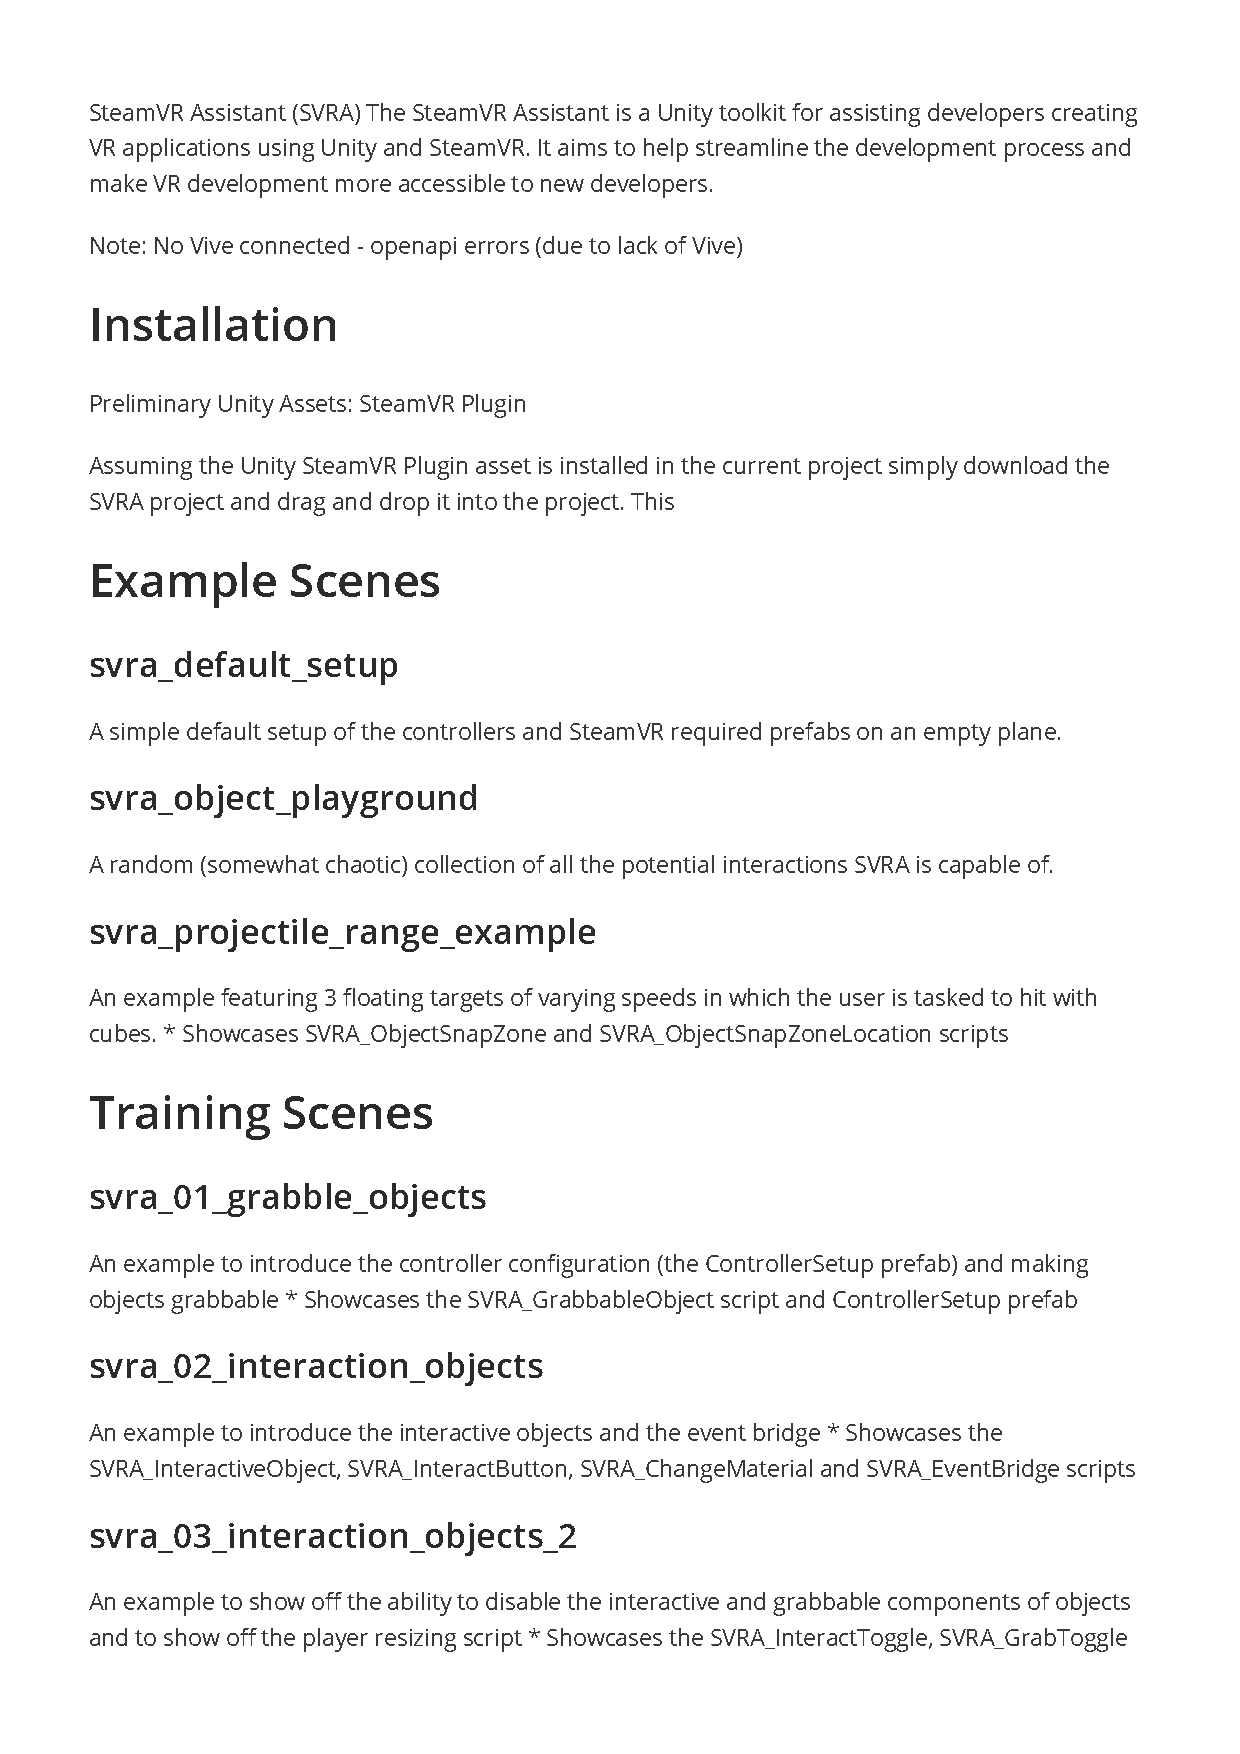
\includepdf[pages=-]{dissertation/pdfs/svradoc.pdf}

\chapter{Evaluation Round 1 Questions}
\label{sec:appendeval1questions}
Included in the following page is a PDF document of the questionnaire produced for the first round of evaluation for the project.

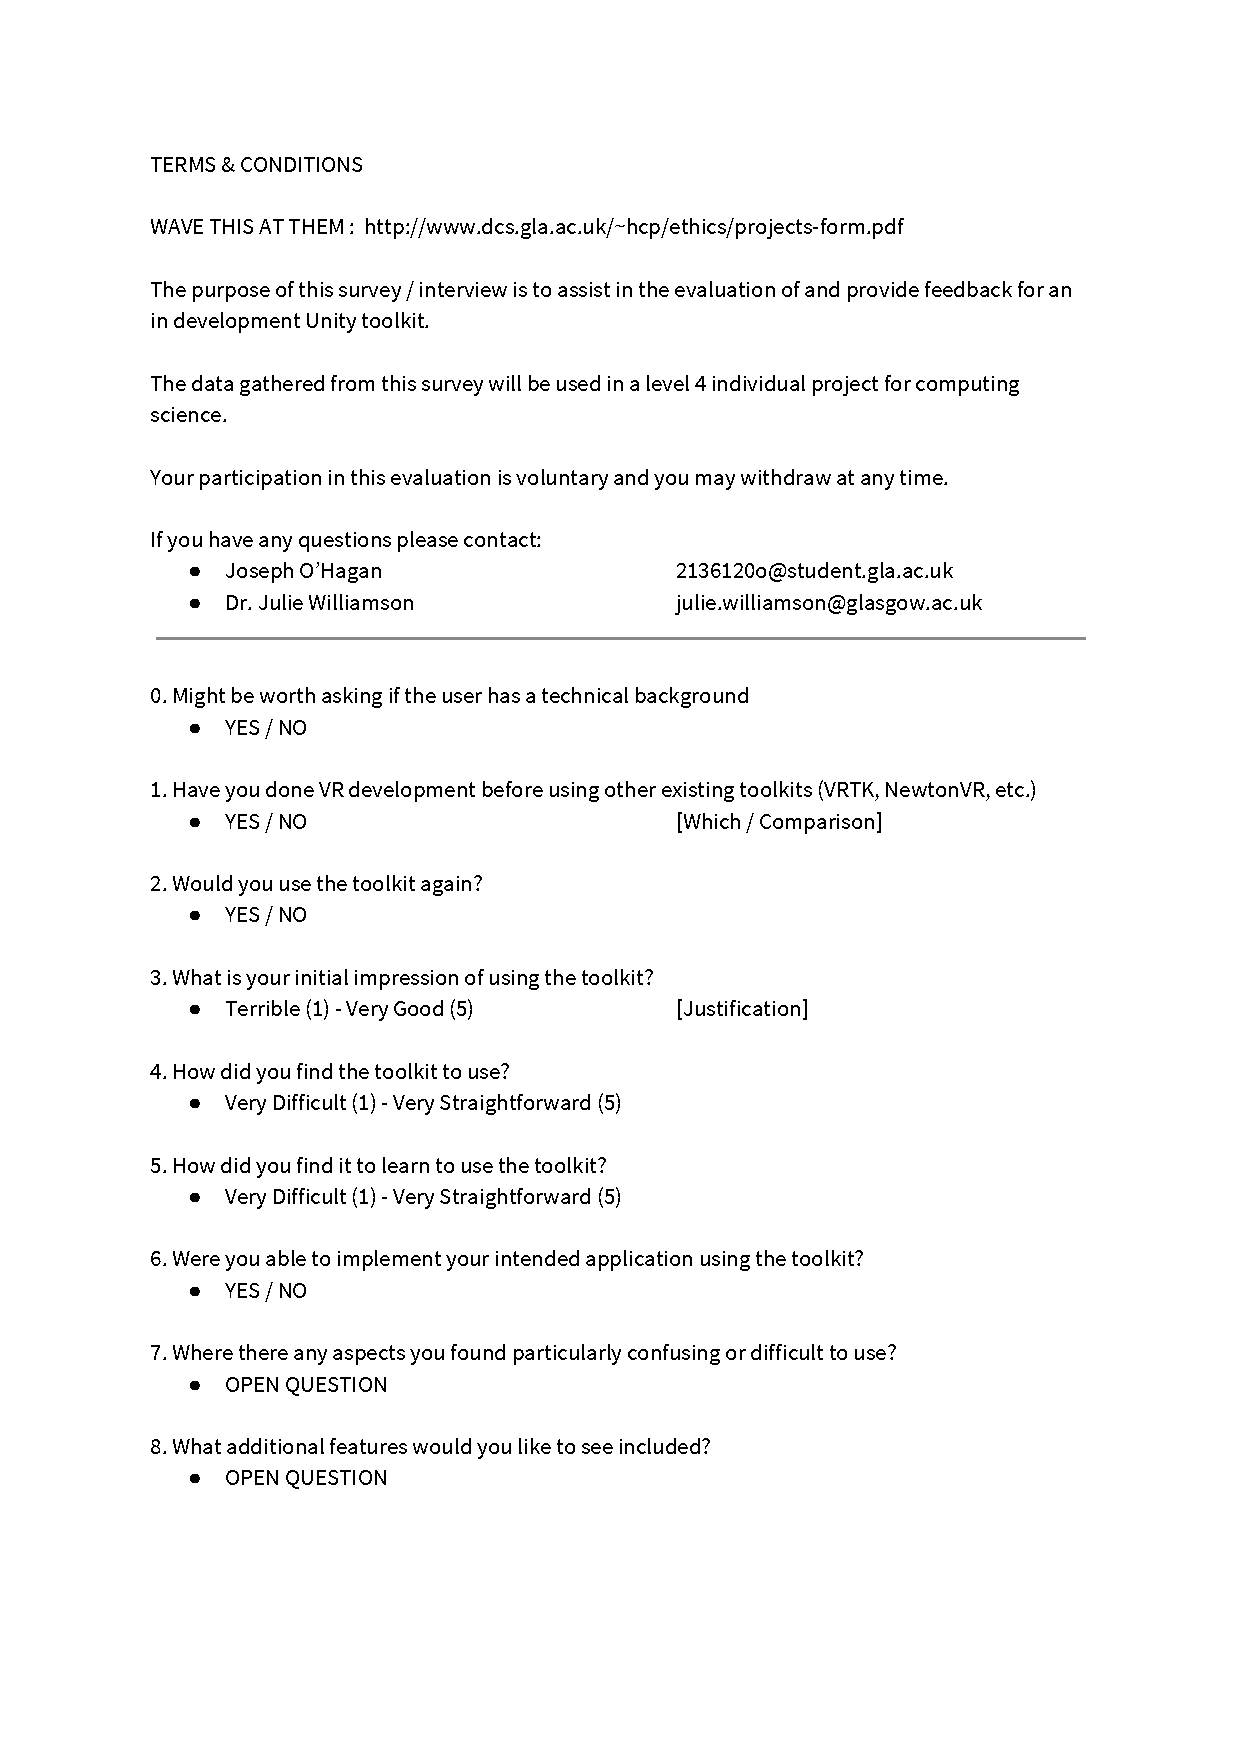
\includepdf[pages=-]{dissertation/pdfs/eval1questions.pdf}

\chapter{Evaluation Round 1 Results}
\label{sec:appendeval1results}
Included in the following pages is the data gathered from the first round of evaluation which was performed on the product. It provides a description of the application built by the participant during the evaluation event followed by the data obtained from the interview with them.

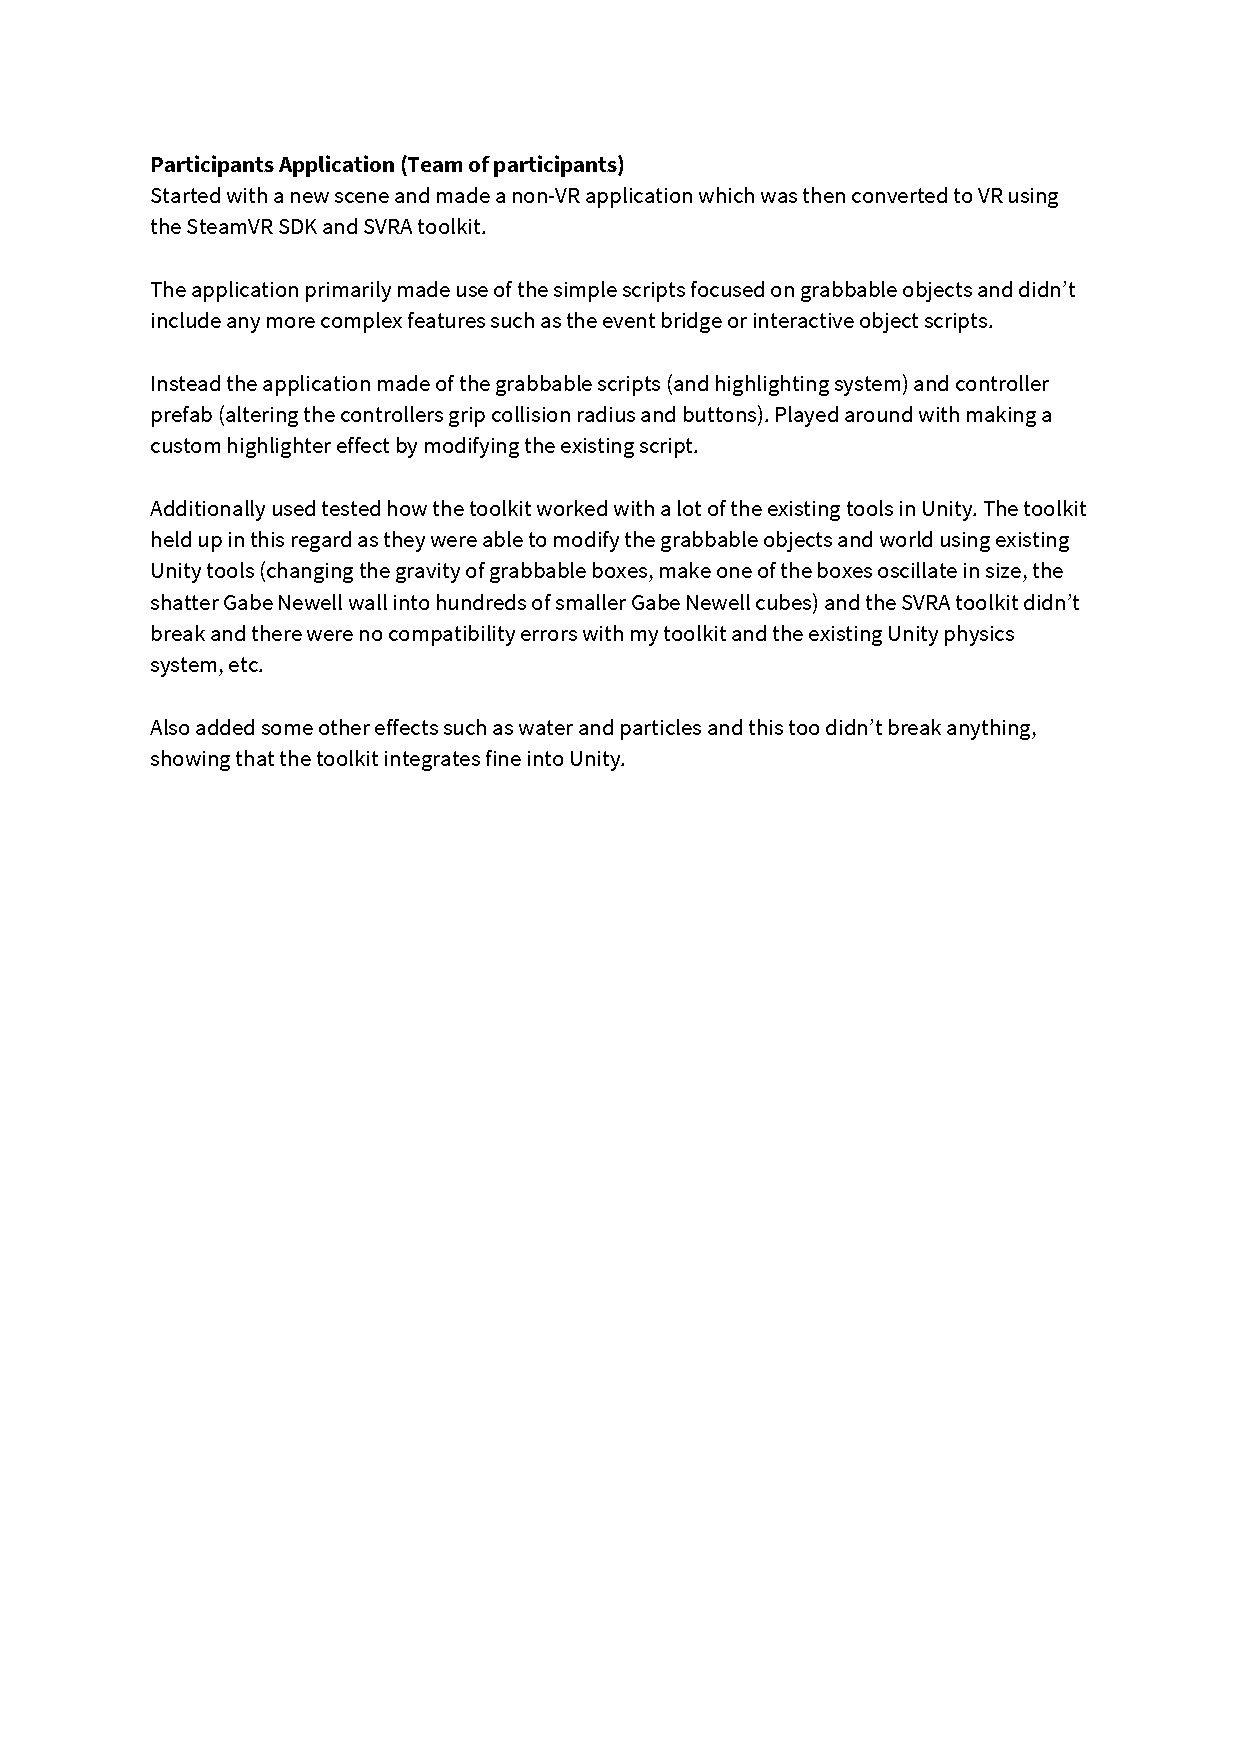
\includepdf[pages=-]{dissertation/pdfs/eval1data.pdf}

\chapter{Evaluation Round 2 Questions}
\label{sec:appendeval2questions}
Included in the following page is a PDF document of the questionnaire produced for the second round of evaluation for the project.

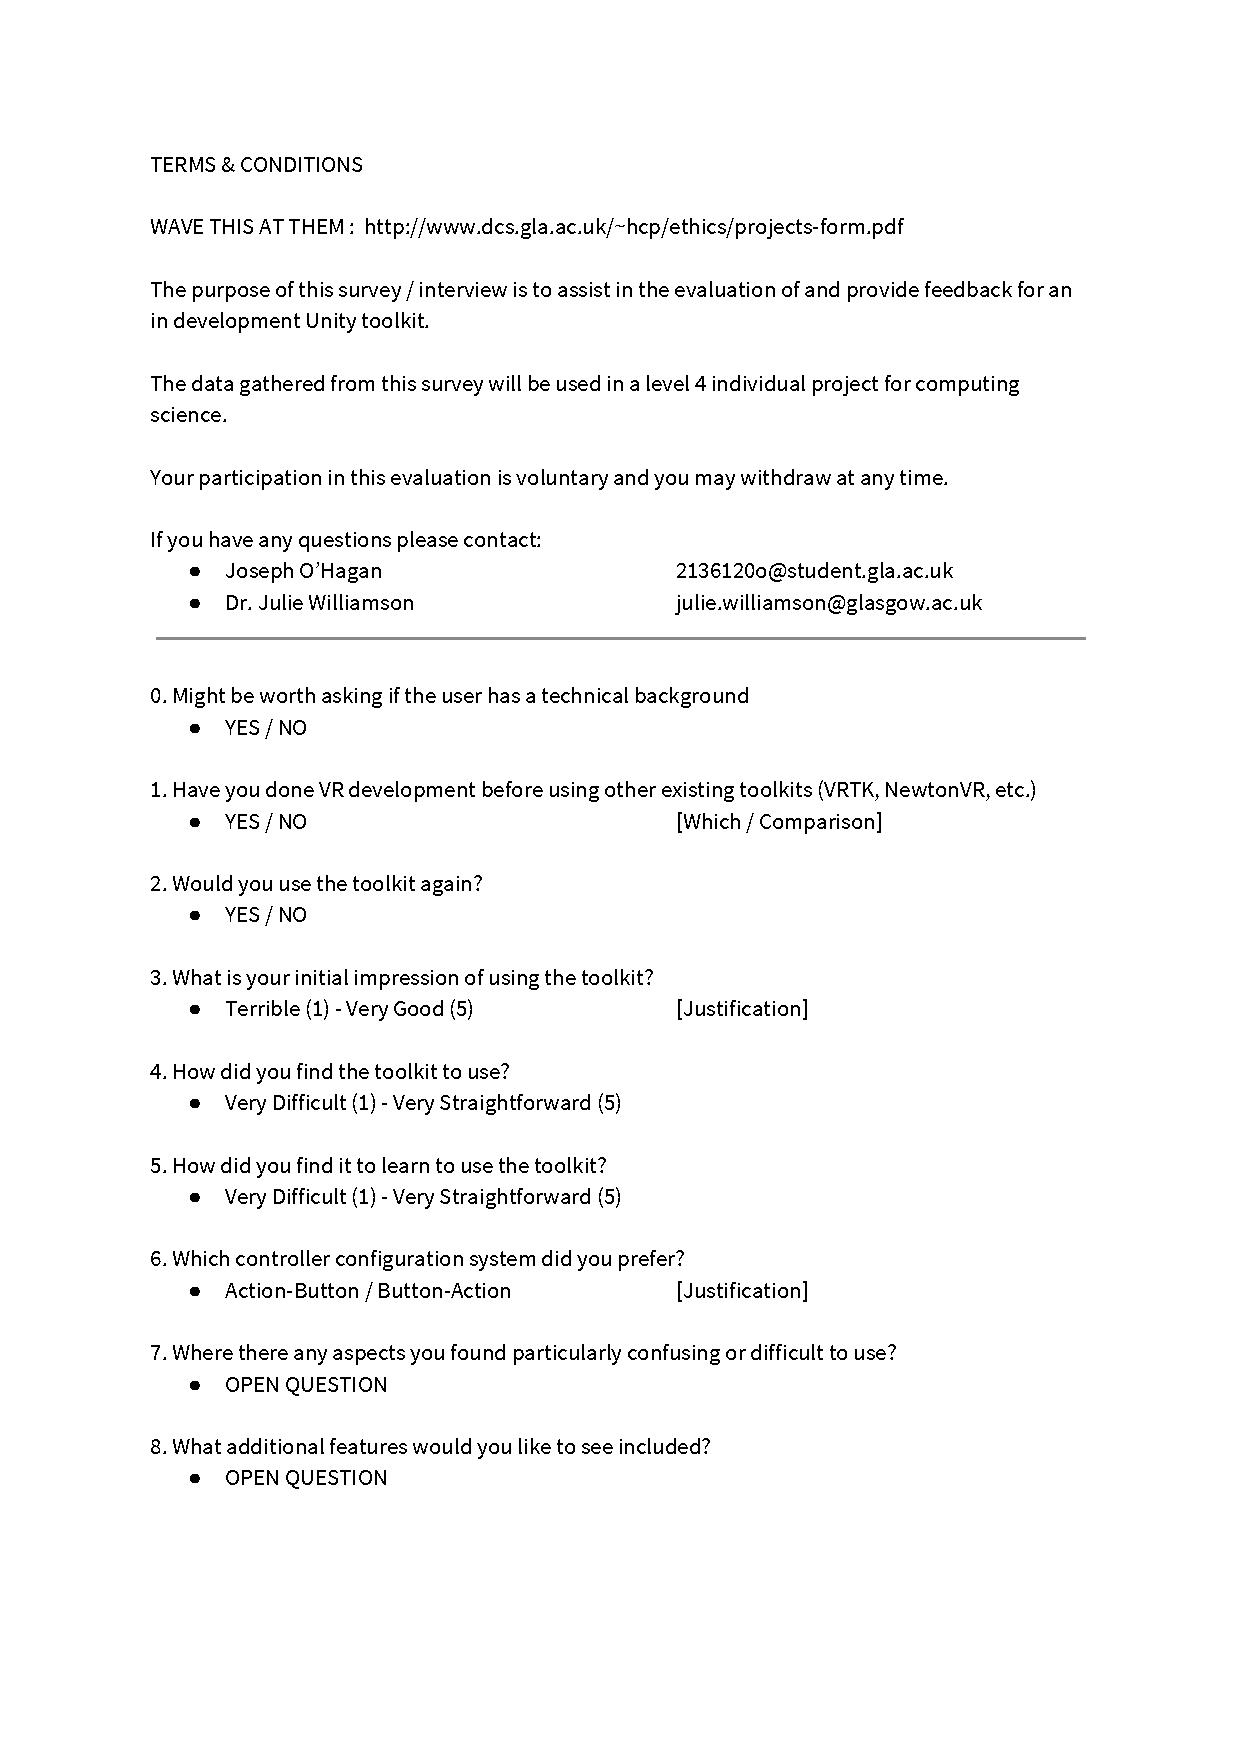
\includepdf[pages=-]{dissertation/pdfs/eval2questions.pdf}

\chapter{Evaluation Round 2 Results}
\label{sec:appendeval2results}
Included in the following pages is the data gathered from the second round of evaluation which was performed on the product.

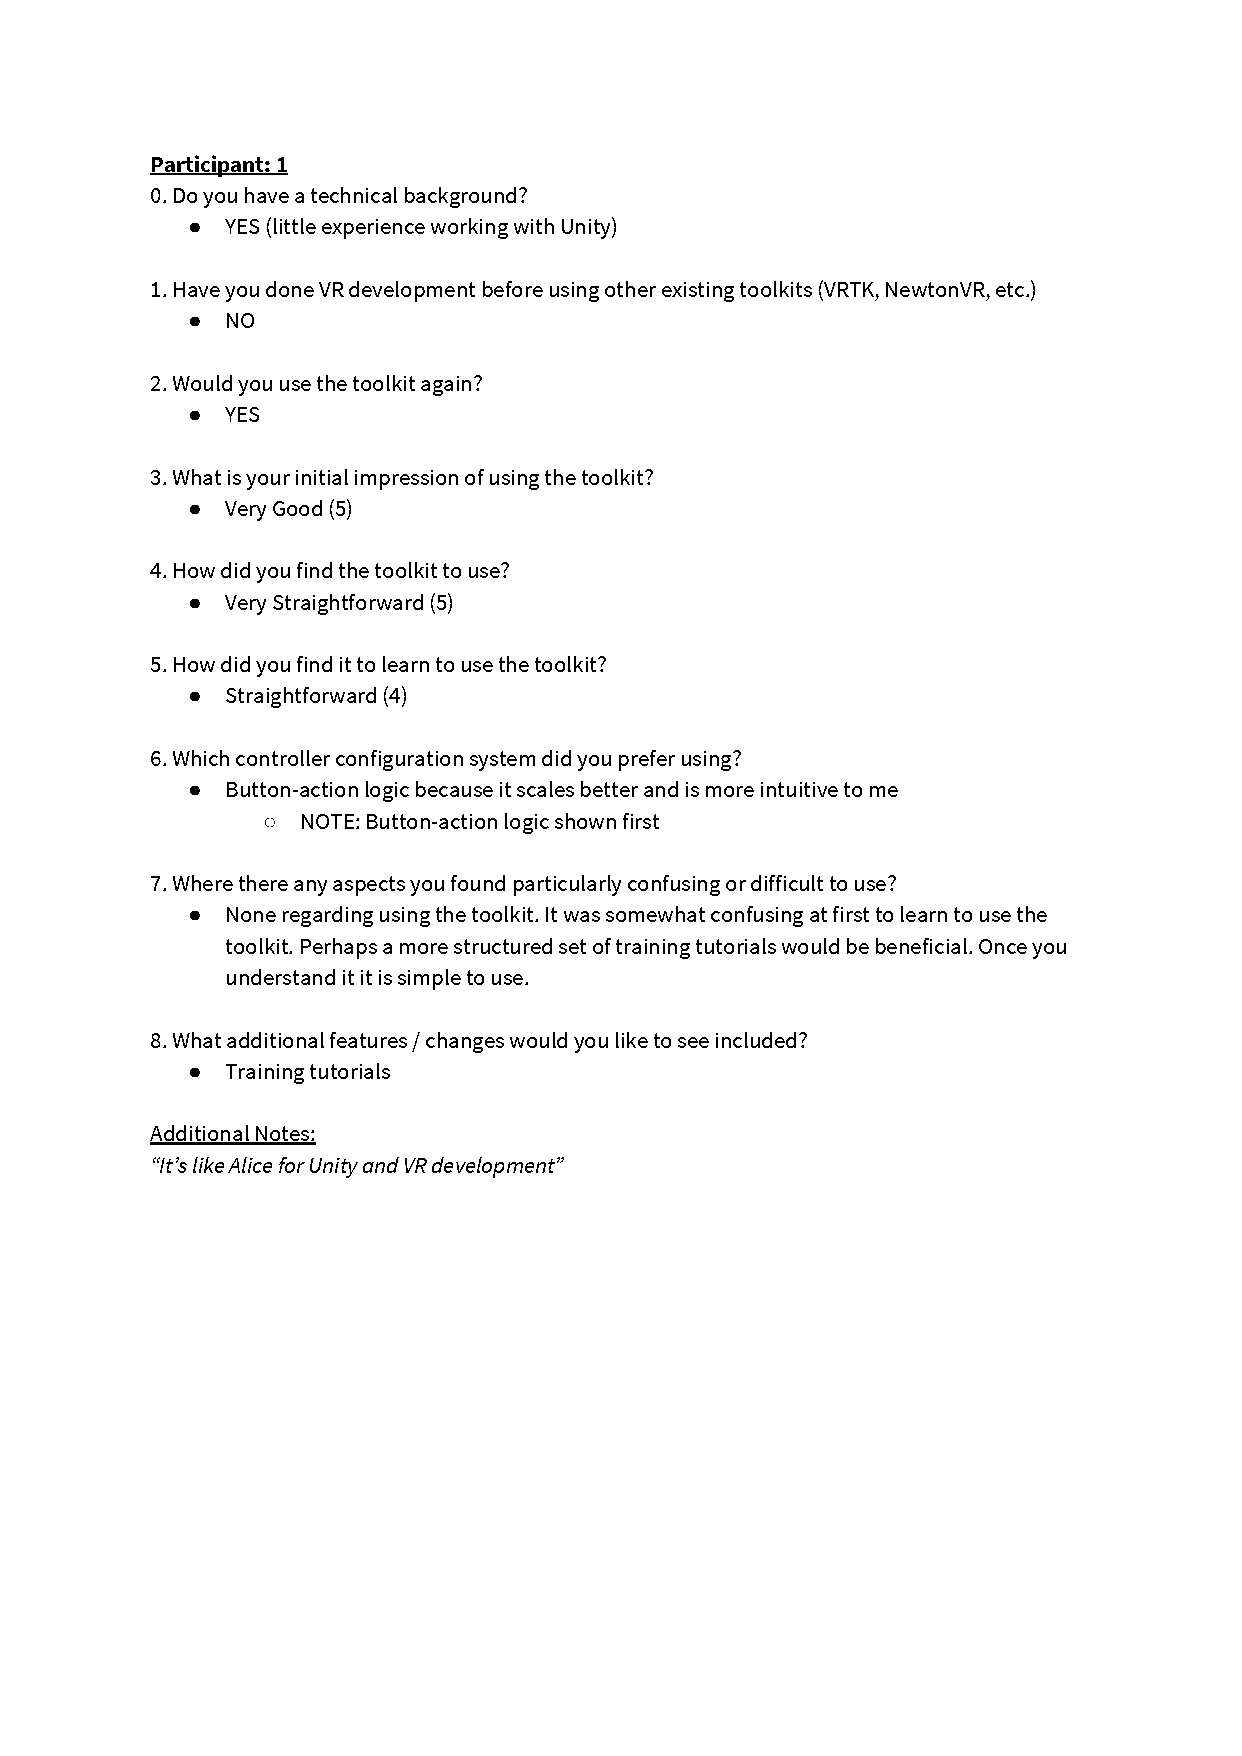
\includepdf[pages=-]{dissertation/pdfs/eval2data.pdf}

\chapter{SVRA Tutorial Sheets}
\label{sec:appendtutorialsheets}
Included in the following pages are the 8 tutorial documents which were produced to help new users learn to use the SVRA toolkit. They begin with the most basic features of the toolkit and increase in complex, slowly introducing the majority of features included within the toolkit.

\includepdf[pages=-]{dissertation/pdfs/SVRA_TutorialSet.pdf}

\chapter{Evaluation Expert Interview Transcript}
\label{sec:appendevalexperttranscript}
Included in the following pages is a condensed transcript document which was produced after the expert interview was conducted during the evaluation of the project.

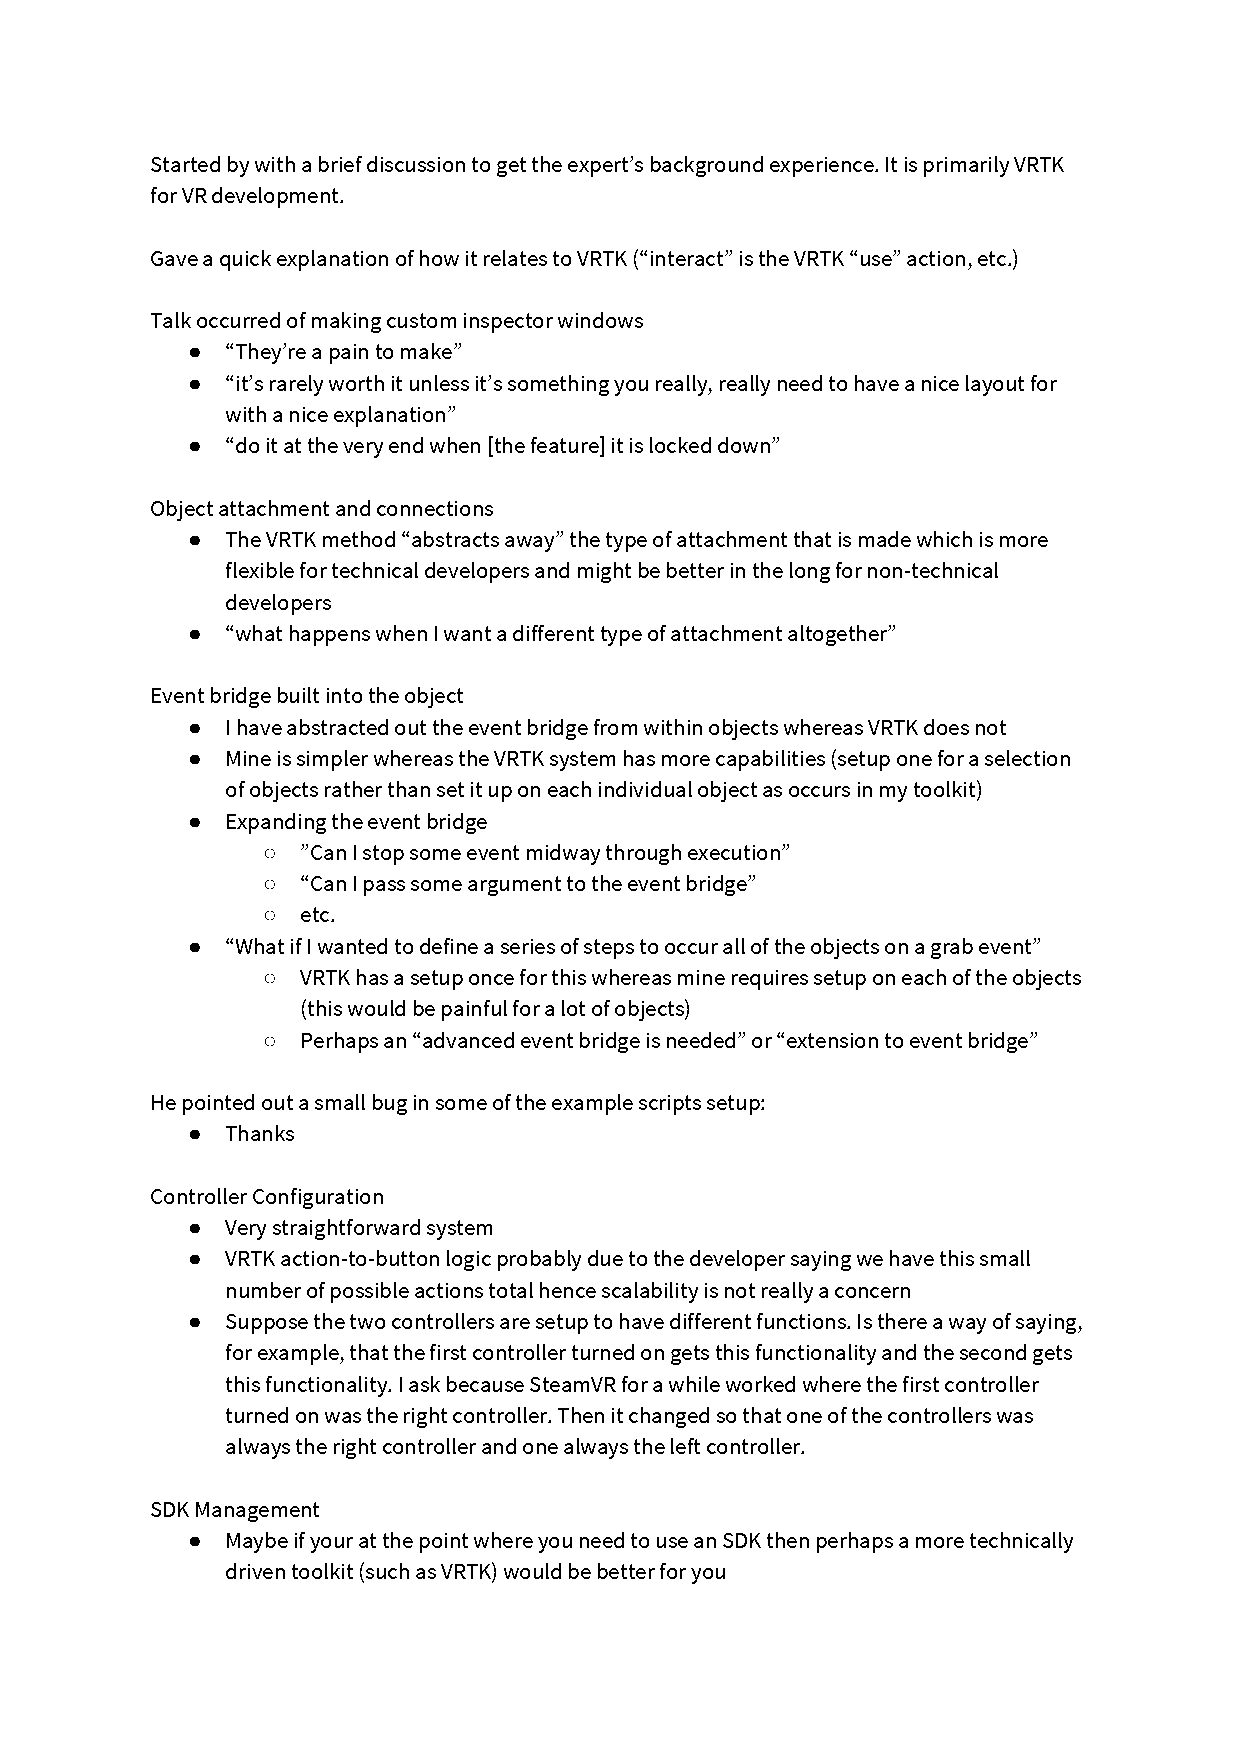
\includepdf[pages=-]{dissertation/pdfs/eval3trans.pdf}

\end{appendices}

%%%%%%%%%%%%%%%%%%%%
%   BIBLIOGRAPHY   %
%%%%%%%%%%%%%%%%%%%%

\bibliographystyle{plain}
\bibliography{bib}

\end{document}
